\documentclass[a4paper, 12pt, master, utf8]{etf}

\usepackage[a4paper, margin=25mm]{geometry}
\usepackage{gentium} % font
\usepackage{enumitem}
\usepackage[linesnumbered, algoruled, longend]{algorithm2e} % za pseudo kod
\usepackage{rotating} % za sidetable

\usepackage{pgfplots}
\usepackage{tikz}
\usepackage{pgf-umlcd}

\usepackage{algpseudocode}
\usepackage{xcolor}
\usepackage{capt-of}
\usepackage{newfloat}
\usepackage{listings} % for code listings

% Configure listings package for Serbian Cyrillic
\lstset{
    basicstyle=\ttfamily\small,
    breaklines=true,
    frame=single,
    numbers=left,
    numberstyle=\tiny,
    showstringspaces=false,
    captionpos=b,
    extendedchars=true,
    inputencoding=utf8,
    literate=%
    {а}{{\cyra}}1 {б}{{\cyrb}}1 {в}{{\cyrv}}1 {г}{{\cyrg}}1 {д}{{\cyrd}}1
    {ђ}{{\cyrdje}}1 {е}{{\cyre}}1 {ж}{{\cyrzh}}1 {з}{{\cyrz}}1 {и}{{\cyri}}1
    {ј}{{\cyrje}}1 {к}{{\cyrk}}1 {л}{{\cyrl}}1 {љ}{{\cyrlje}}1 {м}{{\cyrm}}1
    {н}{{\cyrn}}1 {њ}{{\cyrnje}}1 {о}{{\cyro}}1 {п}{{\cyrp}}1 {р}{{\cyrr}}1
    {с}{{\cyrs}}1 {т}{{\cyrt}}1 {ћ}{{\cyrtshe}}1 {у}{{\cyru}}1 {ф}{{\cyrf}}1
    {х}{{\cyrh}}1 {ц}{{\cyrc}}1 {ч}{{\cyrch}}1 {џ}{{\cyrdzhe}}1 {ш}{{\cyrsh}}1
    {А}{{\CYRA}}1 {Б}{{\CYRB}}1 {В}{{\CYRV}}1 {Г}{{\CYRG}}1 {Д}{{\CYRD}}1
    {Ђ}{{\CYRDJE}}1 {Е}{{\CYRE}}1 {Ж}{{\CYRZH}}1 {З}{{\CYRZ}}1 {И}{{\CYRI}}1
    {Ј}{{\CYRJE}}1 {К}{{\CYRK}}1 {Л}{{\CYRL}}1 {Љ}{{\CYRLJE}}1 {М}{{\CYRM}}1
    {Н}{{\CYRN}}1 {Њ}{{\CYRNJE}}1 {О}{{\CYRO}}1 {П}{{\CYRP}}1 {Р}{{\CYRR}}1
    {С}{{\CYRS}}1 {Т}{{\CYRT}}1 {Ћ}{{\CYRTSHE}}1 {У}{{\CYRU}}1 {Ф}{{\CYRF}}1
    {Х}{{\CYRH}}1 {Ц}{{\CYRC}}1 {Ч}{{\CYRCH}}1 {Џ}{{\CYRDZHE}}1 {Ш}{{\CYRSH}}1
}

% Configure listing name to display "Структура" instead of "Listing"
\renewcommand{\lstlistingname}{Структура}

% Define custom floating environment for code listings
\DeclareFloatingEnvironment[fileext=lol,placement={!ht},name=Структура]{listing}



\addto\extrasserbianc{\def\bibname{Литература}\let\refname\bibname}
\SetAlgorithmName{Псеудо код}{псеудо код}{Листа псеудо кодова}
\SetInd{2mm}{3mm} % za pseudo kod razmak pre i posle
\newcommand*\rot{\rotatebox{90}} % za rotirane labele tabele

\author{Алекса Рачић}

\date{\today}
\title{Евалуација финансијског агента 

користећи велики језички модел

као судију
}
\indeks{2023/3001}
\mentor{проф др. Милош Цветановић}
\usepackage{array}
\newcolumntype{P}[1]{>{\centering\arraybackslash}p{#1}}
\usepackage{titlesec}
\usepackage{setspace}
\usepackage[flushleft]{threeparttable}

\titleformat{\chapter}[display]
  {\normalfont\bfseries}{}{0pt}{\Huge}

\begin{document}

\maketitle

\tableofcontents

\addtocontents{toc}{\protect\thispagestyle{empty}}
\pagenumbering{arabic}
\onehalfspacing
\newpage

% Include chapter files
\chapter{Увод}
\label{sec:1}

\section{Значај финансијских текстуалних података}

Савремени финансијски екосистем генерише огромну количину текстуалних података — од вести у реалном времену и аналитичких извештаја до регулаторних пријава и објава на друштвеним мрежама. Ови неструктурирани текстови носе кључне увиде о тржишним условима и основама пословања компанија, који често утичу на перцепцију и одлуке инвеститора. 

Процењује се да најмање 80\% свих данашњих података чине неструктурирани подаци, што обухвата и наведене финансијске текстуалне токове \cite{rocha_discovering_2021}. Суочавање са овим таласом информација постало је озбиљан изазов: огроман број дневних финансијских вести и извештаја једноставно је немогуће да било који човек у целости прочита и обради. 

Важни детаљи лако могу промаћи када су аналитичари затрпани документима од стотину страница или непрекидним током вести. Због тога је неопходно развијати алате и технике који помажу разумевању и извлачењу увида из великих количина финансијског текста. 

Ефикасна анализа ових текстуалних извора критична је не само за инвеститоре и аналитичаре који желе да доносе информисане одлуке, већ и за регулаторе и истраживаче који се ослањају на квалитативне информације које сирови квантитативни подаци не могу да обухвате.

\section{НЛП и велики језички модели мењају анализу финансија}

Напредак у машинском учењу, а посебно у обради природног језика (НЛП), драматично је променио начин на који финансијска индустрија обрађује текстуалне податке. 

НЛП омогућава рачунарима да тумаче и уносе структуру у неструктуриран текст, претварајући квалитативне информације у квантитативне сигнале или сажетке који су знатно лакши за анализу. 

На пример, задаци који би за човека били изузетно временски захтевни — преглед хиљада новинских чланака ради процене сентимента, читање транскрипата позива поводом зарада ради идентификације кључних тема, или поређење језика у више годишњих извештаја — сада се могу обавити у релативно кратком времену. 

НЛП алати могу брзо да обраде масивне количине текста како би уочили трендове, измерили сентимент и истакли потенцијалне ризике, суштински претварајући људски језик у примењива сазнања \cite{paro_ai_strategic_2023}. 

Кроз рударење и анализу великих текстуалних корпуса, савремени НЛП системи помажу у подршци пословним процесима, откривању макроекономских сигнала и побољшању доношења одлука у финансијским институцијама \cite{yang_evaluating_2025}.

Велики скок у способностима НЛП-а донели су велики језички модели (LLM). То су дубоки модели тренирани на огромним корпусима текста, који омогућавају висок ниво разумевања језика и генерисања текста. 

Модели попут GPT-4 показали су изузетну дубину разумевања, у стању да интерпретирају нијансе финансијског језика и контекста након обуке на великим скуповима текстова \cite{paro_ai_strategic_2023}. 

За разлику од ранијих НЛП система који су често захтевали специфично дотренирање за сваки задатак, LLM-ови могу да решавају широк распон задатака уз минимално или без додатног тренирања, захваљујући општем језичком и светском знању које су усвојили. 

У финансијском домену ови модели могу да произведу организоване, експертске анализе сложених докумената, идући даље од површинске читљивости ка разумевању суптилних детаља и доменске терминологије \cite{yang_evaluating_2025}. 

Један упит LLM-у може да да сажетак годишњег извештаја од 100 страница или одговори на детаљна питања о његовом садржају, практично симулирајући рад искусног финансијског аналитичара.

\section{Улога 10-K извештаја као кључних финансијских докумената}

Међу бројним текстуалним изворима у финансијама, годишњи 10-K извештаји које подносе америчке јавне компаnije издвајају се као посебно важни и информативни. Комисија за хартије од вредности САД (SEC) налаже да компаније поднесу 10-K, свеобухватне годишње извештаје који дају детаљан приказ финансијских резултата и пословних активности фирме \cite{yang_evaluating_2025}. Типичан 10-K садржи ревидиране финансијске извештаје, уз опширне наративне сегменте у којима се разматрају пословни модел и стратегија, тржишни услови, фактори ризика. У суштини, он пружа холистичну и структуирану слику рада и планова компаније. Кључно је да ова документа укључују и квалитативне информације — попут објашњења стратегије и процена ризика — које квантитативне метрике саме по себи не могу да ухвате.

Ипак, 10-K извештаји су озлоглашено обимни и сложени, често имајући стотине страница густог текста, правне терминологије и индустријског жаргона. То их чини тешким за тумачење \cite{yang_evaluating_2025}. Неструктурисана природа наратива отежава проналажење конкретних информација или упоредивост између компанија. Применом техника НЛП-а на 10-K извештајима могу се аутоматски извући корисни увиди и обрасци који би другачије тешко били уочени \cite{yang_evaluating_2025}.

\section{Циљ рада}
Као одговор на наведене изазове и могућности које пружају савремени NLP алати, овај рад је усмерен на развој и евалуацију финансијског агента заснованог на великом језичком моделу (LLM). Конкретно, користимо LLM опште намене уз конструисање контекста како бисмо омогућили агенту да обрађује сложене финансијске документе. Поред самог агента, уводимо и иновативан приступ процене његове успешности: други LLM служи као судија који оцењује и анализира одговоре агента по критеријумима тачности и квалитета. 
\chapter{Теоријски преглед}
\label{sec:2}

\section{Неуронске мреже}
\label{sec:4}

\subsection{Неурон}
\label{sec:4}

У контексту неуронских мрежа, неурон представља основну јединицу обраде информација \cite{noauthor_artificial_20233}. 
Он симулира рад људског неурона у мозгу. Графички изглед једног неурона је приказан на слици \ref{fig:neuron}. 
Сваки неурон прима улазне сигнале $x_0, x_1 ... x_N$, обрађује их, и издаје излазни сигнал $y$.

Тежине (енг. \textit{weights}) $w_0, w_1 ... w_N$ представљају параметре који се користе за модификацију улазних података прослеђених неурону. 
Сваки улаз у неурон је помножен са одговарајућом тежином. Тежине утичу на значајност улазних података и одређују њихову улогу у формирању излаза неурона. 
Процес учења у неуронским мрежама, познат као обука, састоји се из ажурирања и промене тежина како би мрежа најбоље моделовала жељени задатак.

Збир улаза помножених са тежинама сигнала се прослеђује активационој функцији $f$. 
Коришћењем активационих функција, неуронске мреже су у могућности да моделирају нетривијалне односе између улазних и излазних података. 
Овај излазни сигнал затим служи као улаз за следећи слој неурона у мрежи.

Пристрасност (енг. \textit{bias}) је додатни параметар који се користи за прилагођавање излаза неурона. 
Тежина којом пристрасност утиче на активациону функцију је одређена тежином $b$.

\begin{figure}[h]
    \centering
    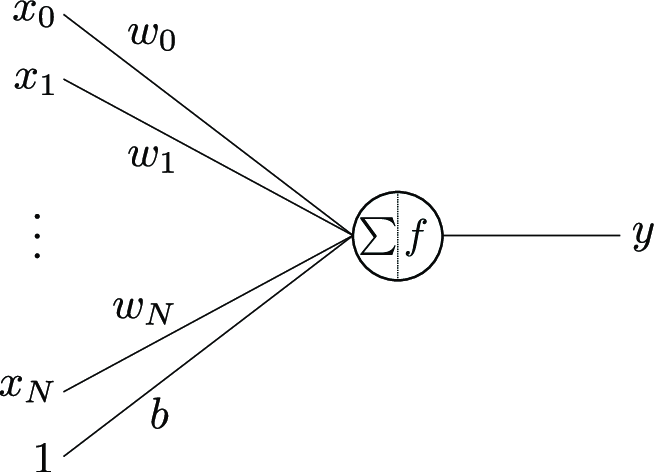
\includegraphics[width=0.7\textwidth]{images/neuron.png}
    \caption{Графички приказ једног неурона \cite{ioannou_structural_2017}}
    \label{fig:neuron}
\end{figure}

Математички израз како тежине, улази и пристрасност утичу на излазни сигнал је дат једначином \ref{eq:neuron}.

\begin{equation}
    y = f\left(\sum_{i=1}^{n} w_i x_i + b\right)
    \label{eq:neuron}
\end{equation}

\subsection{Потпуно повезане неуронске мреже}
\label{sec:41}

Потпуно повезане неуронске мреже (ППНМ) (енг. \textit{Fully Connected Neural Networks}) су скуп повезаних неурона описаних у \ref{sec:4}. 
Састоји се од више слојева, први слој се назива улазни слој, а последњи слој се назива излазни слој. 
Сви остали слојеви се називају скривени слојеви (енг. \textit{hidden layer}). 
На слици \ref{fig:fc} је графички приказана неуронска мрежа која има 2 скривена слоја.
Сваки слој може да има произвољан број неурона, а неуронска мрежа може да има произвољан број скривених слојева. 
Мењајући архитектуру, односно број неурона у једном слоју и број слојева се мења моћ мреже и комплексност задатка који мрежа може да решава.

\begin{figure}[h]
    \centering
    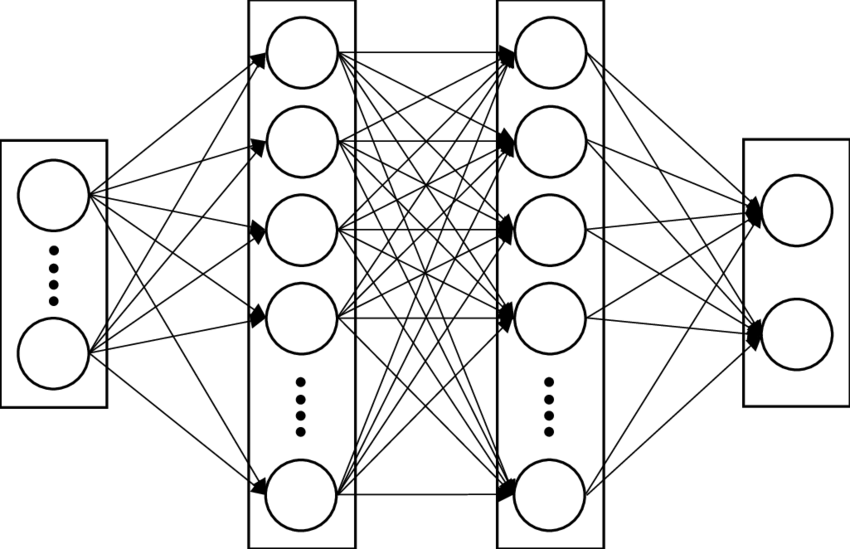
\includegraphics[width=0.7\textwidth]{images/fc.png}
    \caption{Графички приказ потпуно повезане неуронске мреже \cite{anwar_learned_2017}}
    \label{fig:fc}
\end{figure}

ППНМ прима само децималне бројеве као улаз и битно је да приликом тренирања и предикције да исте вредности атрибута улазних података улазе у потпуно повезану мрежу на исти улаз.
Овакав тип мреже се најбоље показао на проблемима класификације \cite{noauthor_artificial_2023}.

\subsection{Софтмакс (\textit{softmax})}

Софтмакс функција се често користи у неуралним мрежама за решавање задатака класификације, као и за генерисање расподеле вероватноћа излаза из мреже. 
Она трансформише илаз тако да све вредности излаза леже у интервалу између 0 и 1 и да се сума свих вредности излаза једнака 1 
Формално, софтмакс функција је дефинисана у изразу \ref{eq:ss} за вектор излаза Z :

\begin{equation}
    \label{eq:ss}
    \text{softmax}(z)_i = \frac{e^{z_i}}{\sum_{j=1}^{N} e^{z_j}}
\end{equation}

Где:

\begin{itemize}
    \item z је вектор излаза модела за сваку од N класа.
    \item e представља експоненцијалну функцију (елемент по елемент).
    \item i је индекс класе за коју рачунамо вероватноћу.
\end{itemize}

\section{Архитектура трансформера}
\label{sec:transformer}

\subsection{Токенизација}

Трансформери раде над дискретним секвенцама токена уместо над сировим текстом, па је први корак токенизација -- разлагање текста на атомске јединице (токене) које чине улаз модела. Савремени модели трансформера често користе токенизацију на нивоу подсегмената (eng. \textit{subword}) како би постигли отворени речник, што значи да се свака реч може представити као секвенца подсекмената токена. Распрострањен \textit{subword} метод је Кодирање парова бајтова (енг. Byte Pair Encoding - BPE), алгоритам за компресију података прилагођен раду са текстом. Првобитно га је представио Gage (1994) за компресију, а касније су га на сегментацију речи применили Sennrich и сар. (2016) \cite{gage_new_1994,sennrich_neural_2016}. Алгоритам итеративно спаја најфреквентнији пар симбола у корпусу, додајући тако насталу целину као нови токен. Понављањем спајања, BPE гради речник уобичајених подсегмената; на пример, ретка реч „nationalism" може се поделити на подсегменте „nation@@" и „alism" (са „@@" као ознака за поделу) на основу фреквенције. Овај процес даје речник фиксне величине састављен од подсегмената које постижу баланс између грануларности на нивоу карактера и холизма на нивоу речи. Теоријска улога токенизације је да ограничи улазни простор на управљив скуп симбола, а да притом сачува могућност да се од тих симбола конструише било која реч.

\subsection{Векторска репрезентација токена}

После токенизације, сваки токен се трансформише у континуалну векторску репрезентацију (енг. \textit{Embedding}). Теоријска улога векторске репрезентације је да омогући моделу да у наученом векторском простору мери семантичке и синтаксичке сличности између токена. Формално, овај слој се може посматрати као табела претраге -- нпр. матрица $\mathbf{E} \in \mathbb{R}^{|V| \times d}$, где је $|V|$ величина речника, а $d$ димензија скривеног слоја модела. Сваки токен $t_i$ мапира се на $d$-димензионални вектор $\mathbf{x}_i = \mathbf{E}[t_i]$. Ови вектори су параметри који се добијају обучавањем модела, иницијално насумични или претходно тренирани, и оптимизују се током обуке модела да би кодирали корисне лингвистичке информације. Код трансформера, вектори су обично величине $d_{\text{model}}$ и скалирају се са $\sqrt{d_{\text{model}}}$ при иницијализацији како би им се величина задржала у разумним границама \cite{vaswani_attention_2017}.

Важно обележје корака векторске репрезентације је додавање позиционог кодирања. За разлику од рекурентних мрежа, трансформер нема урођено поимање редоследа речи, па се позиционе информације морају експлицитно увести. Решење које предлажу Vaswani и сар. је да се сваком позиционом векторском репрезентацијом токена дода позициони вектор \cite{vaswani_attention_2017}. Ова позициона кодирања су фиксна и дефинисана су помоћу синусоидалних функција различитих фреквенција \cite{vaswani_attention_2017}. Конкретно, за позицију $pos$ (нумерисану од 0) и индекс димензије $i$, кодирање је:

\begin{equation}
\text{PE}(pos,\,2i) = \sin\!\Big(\frac{pos}{10000^{2i/d_{\text{model}}}}\Big), \qquad \text{PE}(pos,\,2i+1) = \cos\!\Big(\frac{pos}{10000^{2i/d_{\text{model}}}}\Big)
\label{eq:positional_encoding}
\end{equation}

где је $d_{\text{model}}$ димензионалност ембединга \cite{vaswani_attention_2017}. Ова наизменична синус-косинус формулација производи позиционе векторе јединствене за сваку позицију и који кодирају релативна растојања. Позиционо кодирање $\mathbf{p}_i$ се додаје вектору токена $\mathbf{x}_i$ како би се добила коначна улазна репрезентација $\mathbf{z}_i = \mathbf{x}_i + \mathbf{p}_i$ која се уводи у трансформер. Због тога модел може да разликује позиције токена и учи односе који зависе од редоследа, а да и даље ради над континуалним векторским репрезентацијама.

\subsection{Механизам пажње}

Према научном раду \cite{vaswani_attention_2017}, функција пажње (енг. \textit{Attention head}) се може описати као пресликавање упита и скупа парова кључа и вредности у излазни вектор, при чему су упит, кључеви, вредности и излаз сви вектори. Излаз се израчунава као тежинска сума вектора вредности, а тежина сваке вредности добија се из функције компатибилности између упита и одговарајућег кључа.

\subsection{Скалирана пажња заснована на скаларном производу}

Скалирана пажња заснована на скаларном производу (енг. \textit{Scaled Dot-Product Attention}) је механизам који омогућава моделу да одмери утицај различитих токена при израчунавању репрезентација за следећи слој. У трансформеру, основна јединица је глава пажње са скалираним скаларним производом. Теоријска улога једне главе пажње је да израчуна тежинску комбинацију вектора вредности за сваку позицију, где су тежине одређене паровним сличностима између упита и скупа кључева. Свака глава пажње ради над три скупа вектора: упити ($Q$), кључеви ($K$) и вредности ($V$), димензија $d_k$, $d_k$ и $d_v$ (често $d_v = d_k$) редом. У интроспективној пажњи (енг. \textit{self-attention}), језгру трансформер слојева, упити, кључеви и вредности долазе из исте секвенце, што омогућава моделу да обрађујући дату позицију „обрати пажњу" на друге позиције у секвенци. Механизам пажње израчунава меру компатибилности између сваког упита и сваког кључа помоћу скаларног производа $Q \cdot K^T$ \cite{vaswani_attention_2017}. Резултат се затим скалира са $\frac{1}{\sqrt{d_k}}$ и нормализују \textit{softmax}-ом како би се добиле тежине пажње. Излаз главе пажње је тежинска сума вектора вредности, користећи те нормализоване тежине. Математички, за скуп $Q$, $K$ и $V$, глава пажње даје:

\begin{equation}
\text{Attention}(Q, K, V) = \text{softmax}\!\Big( \frac{Q\,K^T}{\sqrt{d_k}}\Big)\,V
\label{eq:attention}
\end{equation}

како су увели Vaswani и сар. \cite{vaswani_attention_2017}. Сваки ред матрице $\text{softmax}(\frac{QK^T}{\sqrt{d_k}})$ представља расподелу вероватноће над свим кључевима за одређени упит, показујући колико пажње (значаја) упит поклања вредности сваког кључа. Добијена тежинска сума даје контекстни вектор за сваки упит, тј. излаз пажње који кодира информације агрегиране из свих позиција, пристрасно у корист оних релевантних за позицију упита.

Скалирање са $\frac{1}{\sqrt{d_k}}$ је кључан теоријски детаљ. Без њега, скаларни производи $QK^T$ расту по величини са већим $d_k$, што може да доведе тога да \textit{softmax} обрати пажњу на само један токен игноришићи остале. Скалирањем скаларних производа инверзним квадратним кореном димензије кључа, вредности које улазе у \textit{softmax} остају умерене чак и кад $d_k$ расте, што емпиријски води стабилнијем учењу \cite{vaswani_attention_2017,bahdanau_neural_2015}. У пракси, употреба скалиране пажње са скаларним производом у трансформеру обезбедила је једноставнију и бржу имплементацију пажње без жртвовања перформанси \cite{vaswani_attention_2017}. Свака глава пажње стога излази секвенцу вектора (по један по улазној позицији) који мешају информације са свих позиција, фокусирајући се на оне процењене као релевантне датом упиту.

Архитектура механизма пажње је приказама на слици \ref{fig:dot_attention}.

\begin{figure}[h]
    \centering
    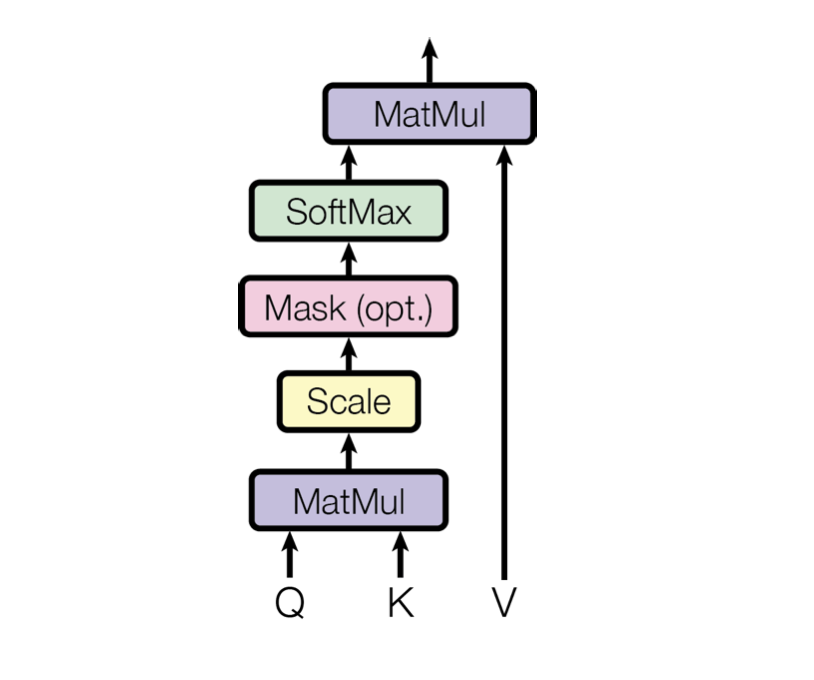
\includegraphics[width=0.7\textwidth]{images/dot-attention.png}
    \caption{Архитектура скалиране пажње засноване на скаларном производу}
    \label{fig:dot_attention}
\end{figure}

\subsection{Механизам пажње са више глава}

Иако једна глава пажње може да извуче један скуп односа преко секвенце, трансформер користи механизам пажње са више глава (енг. \textit{Multi-Head Attention}) како би моделу омогућио да паралелно обраћа пажњу на више аспеката података. Идеја је да постоји више независних глава пажње (рецимо $h$ глава), свака са сопственим линеарним трансформацијама за упите, кључеве и вредности. Улаз у слој вишеглаве пажње се прво пројектује у $h$ различитих подпростора помоћу $h$ научених линеарних пројекција: за сваку главу $i$ имамо матрице пројекција $W_i^Q$, $W_i^K$, $W_i^V$ које мапирају оригиналне $d_{\text{model}}$-димензионалне упите, кључеве и вредности у $d_k$-димензионе $Q_i$, $K_i$, $V_i$. Типично се бира $d_k = d_{\text{model}}/h$ тако да је укупна рачунања преко $h$ глава упоредива са једном „великом" главом по димензионалности. Свака глава $i$ затим изводи скалирану пажњу са скаларним производом у свом пројектованом подпростору, дајући излазну матрицу $\text{head}_i = \text{Attention}(Q_i, K_i, V_i)$ димензије $n \times d_v$ (за $n$ улазних позиција). Излази $h$ глава се конкатенирају (дуж димензије карактеристика), па се кроз завршну линеарну пројекцију $W^O$ (облика $h\cdot d_v$ на $d_{\text{model}}$) поново комбинују информације. У формулном облику, ако $i$-ти излаз главе означимо као $\text{head}_i$, излаз вишеглаве пажње је:

\begin{equation}
\text{MultiHead}(Q, K, V) = \text{Concat}(\text{head}_1, \text{head}_2, \dots, \text{head}_h)\,W^O
\label{eq:multihead}
\end{equation}

где је $\text{head}_i = \text{Attention}(Q W_i^Q, K W_i^K, V W_i^V)$ за $i=1,\dots,h$ \cite{vaswani_attention_2017}. Ова архитектура (слика \ref{fig:multi_head_attention}) ефективно покреће $h$ одвојених слојева пажње у паралели \cite{vaswani_attention_2017}. Теоријска предност вишеглаве пажње је у томе што свака глава може да учи да се фокусира на различите обрасце или односе у подацима.

\begin{figure}[h]
    \centering
    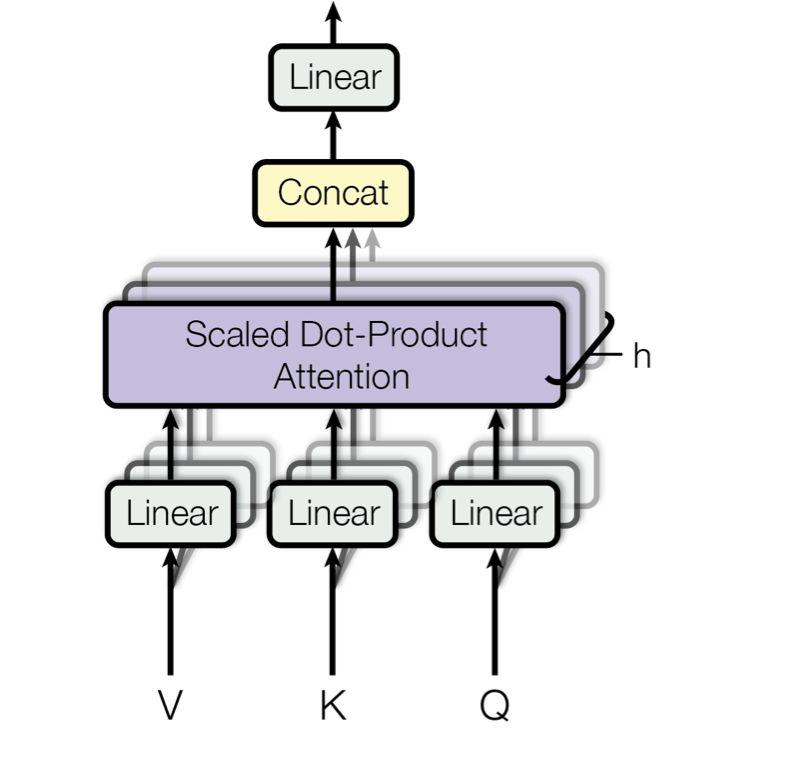
\includegraphics[width=0.7\textwidth]{images/multi-head-attention.png}
    \caption{Архитектура механизма пажње са више глава}
    \label{fig:multi_head_attention}
\end{figure}

\subsection{Трансформер}

У пуном енкодер--декодер Трансформеру (енг. \textit{Transformer}), изворна секвенца се најпре токенизује, ембедује и проширује позиционим кодирањем, након чега пролази кроз стек енкодера од N идентичних слојева. Сваки слој енкодера примењује:

\begin{enumerate}
\item механизам интроспективне пажње (\textit{self-attention}) која омогућава свакој позицији да обраћа пажњу на све остале у извору
\item позиционо-локални, по елементима, потпуно повезан (\textit{feed-forward}) слој
\end{enumerate}

оба подслеја су обавијена резидуалним („Add") везама и нормализацијом слоја („Norm"). Активности вршног слоја енкодера H представљају контекстом богате репрезентације које делују као меморија са адресирањем по садржају за декодер. Декодер конзумира на десно померену циљну секвенцу са сопственом векторском репрезентацијом и позиционим кодирањем. Сваки слој декодера садржи:

\begin{enumerate}
\item маскирану самопажњу, са каузалном (троугластом) маском тако да позиција $t$ не може да види токене $> t$
\item енкодер--декодер \textit{cross-attention}, где упити декодера претражују меморију енкодера N (кључеве/вредности), омогућавајући ослањање на извор
\item \textit{feed-forward} мрежу
\end{enumerate}

и овде резидуалне путање и нормализација слоја стабилизују оптимизацију и очувавају сигнал. Слагање слојева даје хијерархијску композицију: нижи слојеви хватају локалне синтаксичке сигнале, док виши кодирају семантичке односе, при чему механизам пажње са више глава расподељује ове улоге по главама. Коначна стања декодера пролазе кроз линеарну пројекцију и \textit{softmax} (енг. \textit{softmax}) ради добијања вероватноћа наредног токена.

Графички приказ архитектуре трансформера је приказана на слици \ref{fig:transformer}.

\begin{figure}[h]
    \centering
    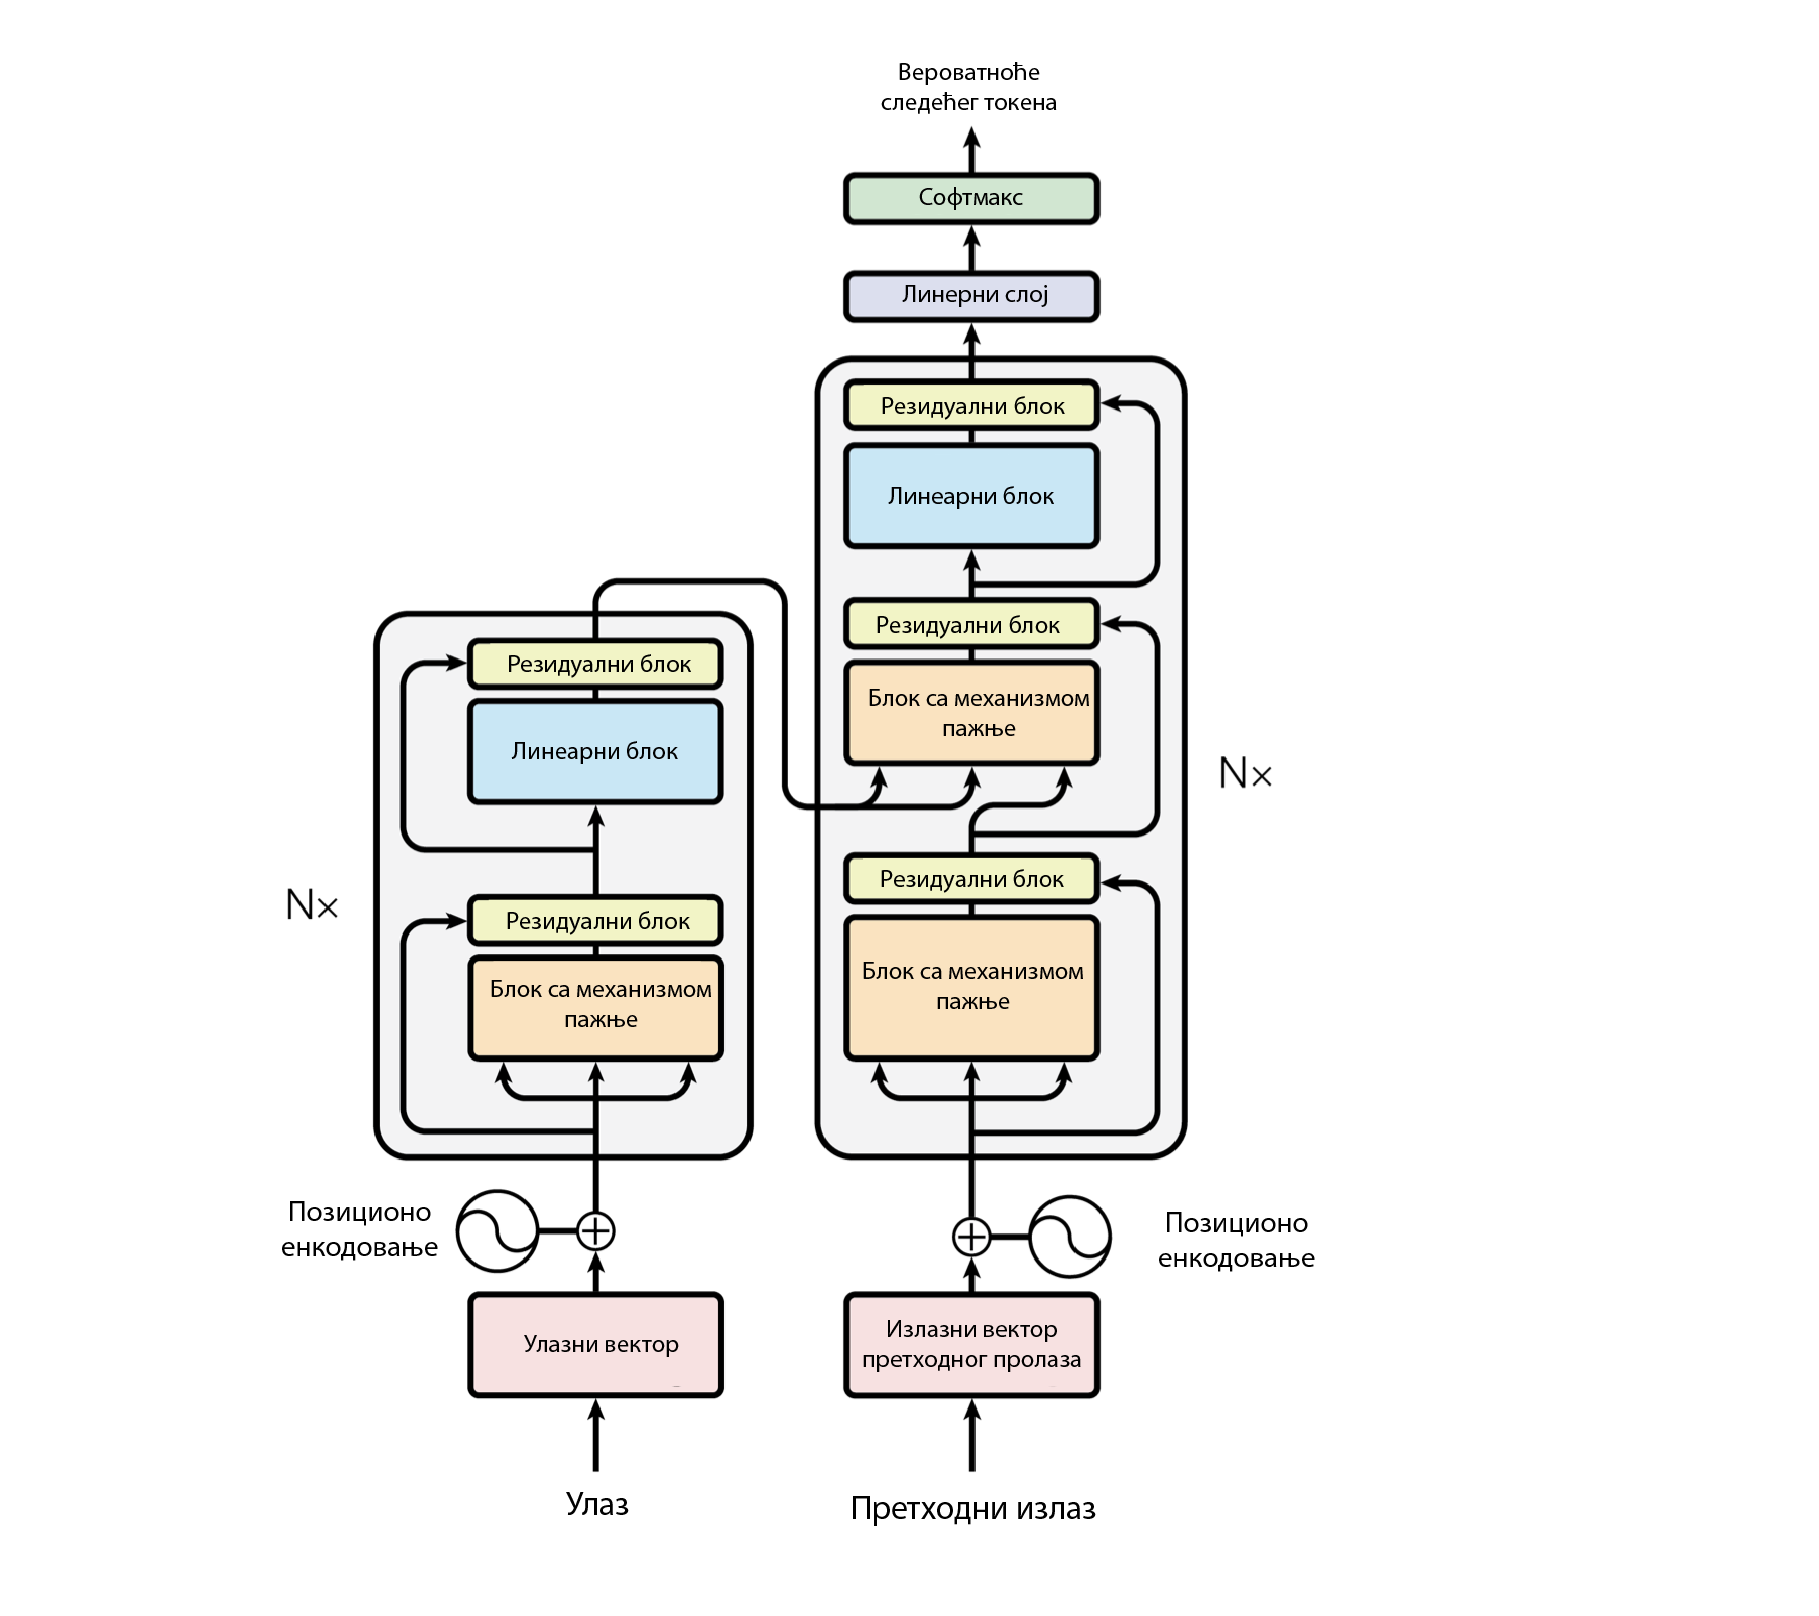
\includegraphics[width=0.9\textwidth]{images/transformer.png}
    \caption{Архитектура трансформера}
    \label{fig:transformer}
\end{figure}

\section{Архитектура великог језичког модела}
\label{sec:llm_architecture}

Велики језички модели (ВЈМ) (енг. \textit{Large Language Models - LLM}) заснивају се на трансформер архитектури \cite{vaswani_attention_2017}. ВЈМ је веома дубока хрпа трансформер слојева, при чему сваки слој садржи вишеглаву пажњу и \textit{feed-forward} подслојеве. Ова архитектура омогућава моделу да одмерава релевантност сваке речи (токена) у улазу у односу на све друге речи, хватајући далекосежне зависности у тексту. Пошто трансформер обрађује речи паралелно, може да се скалира на веома велике величине модела и ефикасно рукује дугим секвенцама \cite{vaswani_attention_2017}.

\subsection{Врсте великих језичких модела}

Иако основни трансформер блок остаје језгро, ВЈМ-ови типично имају огроман број параметара распоређених преко многих слојева. На пример, модел GPT-3 компаније OpenAI садржи 175 милијарди параметара и користи 96 трансформер слојева у конфигурацији само-декодера \cite{brown_language_2020}. Сваки слој у GPT-3 има бројне главе пажње (96 глава по слоју) које раде паралелно, што омогућава моделу да прати различите аспекте улазног текста \cite{brown_language_2020}.

Упркос својој величини, архитектура већине ВЈМ-а може се категоризовати у неколико основних типова:

\begin{itemize}
\item \textbf{само-декодерски модели} (попут серије GPT и Meta-иног LLaMA) који генеришу текст предвиђајући следећи токен
\item \textbf{само-енкодерски модели} (попут BERT-а) намењени задацима разумевања и анализе
\item \textbf{енкодер--декодер модели} (попут T5) погодни за секвенца-у-секвенцу задатке (превођење, сажимање итд.) \cite{vaswani_attention_2017,lu_large_2024}
\end{itemize}

Општенаменски ВЈМ који се користе у чет-ботовима и креативном генерисању текста обично су трансформери само-декодерског типа, претходно тренирани да настављају текст. У свим случајевима, међутим, оквир самопажње трансформера је кичма која омогућава овим моделима да из података науче сложене језичке обрасце и семантику \cite{vaswani_attention_2017}. Резултат је архитектура која, када се скалира, може да испољи изненађујуће богате способности разумевања и генерисања језика.

\subsection{Ограничења великих језичких модела}

Однос између дужине контекста и механизма пажње трансформера је директан. Механизам интроспективне пажње омогућава сваком токену да обрати пажњу на све друге токене у улазу, што је начин на који модел интегрише контекст. Али то има цену: пажња има квадратну сложеност у односу на дужину секвенце. Другим речима, удвостручавање прозора контекста може да учетворостручи потребно рачунање за пажњу \cite{vaswani_attention_2017,lu_large_2024}. Зато је дужина контекста дуго имала практична ограничења -- обрада веома дугих секвенци је спора и захтева много меморије. Тренутни ВЈМ-и се претежно тренирају на релативно кратким исечцима текста (нпр. неколико хиљада токена), што такође значи да можда природно не уче зависности у веома дугим текстовима \cite{lu_large_2024}.

%\chapter{Литература}
%\label{sec:7}

% Predlažem upotrebu bibtex i kreiranje .bib fajlova, a da se podaci za njh skidaju sa Google Scholar i sličnih servisa
\section{Контекст у великим језичким моделима}
\label{sec:llm_context}

У ВЈМ-а, контекст се односи на улазни текст који се моделу пружа и на који се модел условљава да би генерисао одговор. То чини ефективну радну меморију модела, ограничену прозором контекста одређене дужине мерене у токенима, што ограничава колико текста модел може одједном да разматра \cite{martineau_whats_2024}. Све инструкције задатка, позадинске информације и историја конверзације морају бити кодиране у овом контексту, јер LLM-ови током инференције не уче активно нове информације – уместо тога, генеришу излазе искључиво на основу образаца у датом упиту и својих тренираних параметара \cite{martineau_whats_2024}. Другим речима, све што модел треба да зна или да уради за дати упит мора бити обезбеђено у улазном контексту у тренутку извршавања. Већи прозор контекста зато омогућава да се укључи више информација или дужи дијалог, помажући моделу да током дугих интеракција производи кохерентне и релевантне одговоре \cite{martineau_whats_2024}. Међутим, преоптерећивање контекста има мане: повећава рачунање и трошак, а модели могу тешко да уоче релевантне детаље ако је промпт предугачак или има велики шум \cite{liu_lost_2023}. Истраживања показују да ВЈМ-и често испољавају пристрасности првенства и свежине – теже да се фокусирају на информације на почетку или крају прозора контекста више него на оне у средини \cite{liu_lost_2023}. Ово сугерише да редослед и позиционирање садржаја у промпту могу утицати на перформансе модела, што је важна напомена при изради ефективних упита \cite{liu_lost_2023}.

\subsection{Манипулисање контекстом путем изградње упита}

Пошто је понашање ВЈМ-а у потпуности вођено улазним текстом, могуће је манипулисање контекстом како би се модел усмерио ка различитим задацима и одговорима. Ова пракса је позната као промпт инжењеринг (енг. \textit{Prompt engineering}): формулисање правих инструкција или примера у промпту да би се изазвао жељени излаз модела. Уместо ажурирања параметара модела, промпт инжењеринг „програмира" модел природним језиком. Промптови могу бити једноставни – инструкција или питање – или сложени, са структурираним уносом који садржи више примера и ограничења. На пример, може се испред текста додати инструкција као што је „Преведи следећи текст на француски:" или „Сажми кључне тачке из овог чланка." да би се задатак усмерио \cite{sahoo_systematic_2025}. Ова способност извођења задатака по примеру у контексту, без додатног тренирања модела, обележје је модерних ВЈМ-а и често се назива учење у контексту (енг. \textit{in-context learning}) \cite{sahoo_systematic_2025}.

\paragraph{Технике манипулисања контекстом укључују:}

\begin{itemize}
  \item \textbf{Zero-Shot промптовање:} Пружање само инструкције или питања, ослањајући се на стечено знање модела за одговор (нпр. „Објасни зашто је небо плаво.") \cite{sahoo_systematic_2025}.
  \item \textbf{Few-Shot промптовање:} Давање неколико примера питање--одговор или демонстрација пре стварног упита, да би се моделу показало како да одговара. Ово помаже да се активирају релевантни обрасци из предтренинга путем примера \cite{sahoo_systematic_2025}.
  \item \textbf{Chain-of-Thought промптовање:} Инструкција моделу да резонује кроз проблем корак--по--корак (често додавањем „Хајде да размишљамо корак по корак") ради побољшања тачности у сложеном резоновању \cite{sahoo_systematic_2025}.
  \item \textbf{Промптовање улогом:} Додавање контекста који уоквирује ко је модел или стил одговора (нпр.: „Ти си стручни медицински асистент. Одговори на питање уз клиничке доказе.") \cite{sahoo_systematic_2025}.
\end{itemize}

Стратешким обликовањем контекста овим методама, из истог модела могу се откључати широки опсези способности – од писања кода до одговарања на финансијска питања – без промене самог модела \cite{sahoo_systematic_2025}.

\subsection{Генерисање са допунским преузимањем}

Иако се промпт дизајном може боље искористити оно што ВЈМ већ зна, постоје ситуације када су потребне информације које модел не зна. Генерисање са допунским преузимањем (енг. \textit{Retrieval--Augmented Generation} -- RAG) је техника која ово ограничење превазилази увођењем спољног извора знања у контекст који се даје моделу \cite{lewis_retrieval_2020}. У овом приступу, систем најпре шаље упит ка бази знања или корпусу докумената да дохвати релевантне пасусе, а затим проширује промпт тим преузетим пасусима као додатним контекстом \cite{lewis_retrieval_2020}. LLM се затим условљава овим обогаћеним контекстом да би генерисао одговор \cite{lewis_retrieval_2020}. То ефективно опрема модел динамичком, непараметарском меморијом: уместо да се ослања само на оно што је у његовим фиксним параметрима, модел може да користи ажурне информације довучене у тренутку упита \cite{lewis_retrieval_2020}.

Оваквим проширивањем контекста може значајно да се побољша учинак на задацима који захтевају знање. На пример, показано је да је RAG модел достигао добре резултате на бенчмарцима за отворене и доменске задатке са структуром питање--одговор тако што је за сваки упит преузимао релевантне исечке са Википедије \cite{lewis_retrieval_2020,yang_dual_2025}. Поред тога, ажурирање знања модела више не захтева скупо поновно тренирање -- довољно је освежити или проширити спољну базу знања, а механизам за преузимање ће довести нове информације у контекст модела \cite{lewis_retrieval_2020}.

Важно је уочити однос између генерисања са допунским преузимањем и величине прозора контекста ВЈМ-а \cite{kim_large_2024}. Када би се, хипотетички, цела база знања или многи документи могли сместити у промпт, модел би у теорији могао директно да приступи свим тим информацијама без засебног корака преузимања \cite{kim_large_2024}. Ипак, постоје практични изазови: веома велики контексти носе велике трошкове и могу довести до превеликог шума у контексту \cite{liu_lost_2023,kim_large_2024}. Стога ова техника постаје веома релевантна, нарочито за упите који захтевају прецизно издвајање мале количине релевантног знања из огромног корпуса или за праћење најновијих информација као што је случај са финансијским извештајима.
\chapter{Подаци}
\label{sec:3}

\section{Преглед базе података EDGAR}
\label{secsec:3}

Програм електронског прикупљања, анализе и повлачења (енг. \textit{Electronic Data Gathering, Analysis, and Retrieval} - EDGAR) је примарна база података Комисије за хартије од вредности Сједињених Америчких Држава (SEC) за финансијске пријаве. Све јавне компаније дужне су да своје изјаве, периодичне извештаје и друге обрасце за обелодањивање података подносе путем EDGAR-а, уместо папирних пријава. EDGAR ове пријаве чини бесплатно доступним јавности, омогућавајући инвеститорима да преузимају и претражују хиљаде докумената компанија и фондова.

\subsection{Врсте извештаја доступних на EDGAR-у}

EDGAR организује пријаве према стандардизованим типовима образаца. Кључни извештаји доступни у бази EDGAR укључују:

\begin{itemize}
\item \textbf{Образац 10-K (енг. \textit{Form 10-K}) (Годишњи извештај):} Свеобухватан годишњи извештај који америчке јавне компаније морају да поднесу након завршетка сваке фискалне године. Образац 10-K садржи ревидиране годишње финансијске извештаје, дискусију о пословању компаније и материјалним факторима ризика, као и менаџментову дискусију и анализу финансијских резултата за годину.

\item \textbf{Образац 10-Q (енг. \textit{Form 10-Q}) (Квартални извештај):} Краћи извештај који се подноси за фискални квартала. Образац 10-Q укључује кварталне финансијске извештаје, ажурирања о свим значајним променама или материјалним ризицима од последњег 10-K/10-Q.

\item \textbf{Образац 8-K (енг. \textit{Form 8-K}) (Текући извештај):} Извештај који се подноси ради обелодањивања великих корпоративних догађаја у реалном времену, уместо чекања на наредни 10-Q или 10-K. Компаније подносе 8-K кад год се догоде значајни догађаји које акционари треба да знају.
\end{itemize}

\section{Преглед форме годишњег извештаја 10-K}

Образац 10-K је годишњи извештај који прописује SEC и који америчке јавне компаније подносе, а нуди детаљну слику финансијског стања и пословних активности компаније током претходне године. 10-K укључује темељан опис пословних операција компаније, дискусију о ризицима са којима се компанија суочава, и ревидиране финансијске резултате за фискалну годину. Менаџмент компаније такође пружа анализу и контекст за финансијске резултате, објашњавајући покретаче перформанси и све трендове или неизвесности који би могли утицати на будуће резултате.

\subsection{Садржај и структура извештаја Форма 10-K}

Форма 10-K је подељена на четири главна дела, при чему сваки део садржи неколико ставки како је прописано регулативом SEC-а. Укупно, постоји 15 нумерисаних ставки које морају бити обухваћене у 10-K. У наставку је преглед ових делова и информација које сваки садржи:

\subsubsection{Део I – Преглед пословања и ризика}

\begin{itemize}
\item \textbf{Ставка 1. Пословање (енг. \textit{Item 1. Business}):} опис операција, главни производи/услуге, зависна друштва, тржишта, конкуренција, регулатива, сезоналност.

\item \textbf{Ставка 1А. Фактори ризика (енг. \textit{Item 1A. Risk Factors}):} најзначајнији ризици по компанију/хартије, набројани по значају.

\item \textbf{Ставка 1Б. Нерешени коментари особља (енг. \textit{Item 1B. Unresolved Staff Comments}):} материјални нерешени коментари Комисије за хартије од вредности (SEC).

\item \textbf{Ставка 2. Непокретности (енг. \textit{Item 2. Properties}):} значајна физичка имовина (погони, капацитети, рудници, канцеларије, некретнине).

\item \textbf{Ставка 3. Судски спорови (енг. \textit{Item 3. Legal Proceedings}):} парнице и судски поступци.

\item \textbf{Ставка 4. Обелодањивања о безбедности у рудницима (енг. \textit{Item 4. Mine Safety Disclosures}):}
\end{itemize}

\subsubsection{Део II – Финансијске информације и резултати}

\begin{itemize}
\item \textbf{Ставка 5. Тржиште акција и питања акционара (енг. \textit{Item 5}):} берзе, број акционара, политика дивиденди, откупи и емисије.

\item \textbf{Ставка 6. Одабрани финансијски подаци (енг. \textit{Item 6. Selected Financial Data}):} кључни показатељи (обично последњих 5 година) у сажетку.

\item \textbf{Ставка 7. Коментари менаджмента (енг. \textit{Item 7. Management's Discussion and Analysis}):} анализа стања и резултата, ликвидност, ресурса, трендова и неизвесности као и кључне процене.

\item \textbf{Ставка 7А. Тржишни ризик (енг. \textit{Item 7A. Quantitative and Qualitative Disclosures About Market Risk}):} изложености (каматни, девизни, робни, цена капитала) и управљање ризицима.

\item \textbf{Ставка 8. Финансијски извештаји и додатни подаци (енг. \textit{Item 8}):} Биланс стања, биланс успеха, извештај о токовима готовине и капитал.

\item \textbf{Ставка 9. Промене и неслагања са рачуновођама (енг. \textit{Item 9}):} промена ревизора и материјална неслагања.

\item \textbf{Ставка 9А. Контроле и процедуре (енг. \textit{Item 9A. Controls and Procedures}):}

\item \textbf{Ставка 9Б. Остале информације (енг. \textit{Item 9B. Other Information}):} информације које су требале у Форми 8-K у Q4, а нису објављене.
\end{itemize}

\subsubsection{Део III – Руководство и управљање}

\begin{itemize}
\item \textbf{Ставка 10. Директори, извршни руководиоци и корпоративно управљање (енг. \textit{Item 10}):} биографије, кодекс етике, структура одбора/чланства.

\item \textbf{Ставка 11. Накнаде извршних руководилаца (енг. \textit{Item 11. Executive Compensation}):} плате, бонуси, акцијске награде, политике програма.

\item \textbf{Ставка 12. Власништво и питања акционара (енг. \textit{Item 12. Security Ownership}):} власништво >5\%, руководиоци/директори; планови капиталних компензација.

\item \textbf{Ставка 13. Повезана лица и независност директора (енг. \textit{Item 13. Certain Relationships}):} материјалне трансакције са инсајдерима и независност директора.

\item \textbf{Ставка 14. Накнаде и услуге главног рачуновође (енг. \textit{Item 14. Principal Accountant Fees and Services}):} накнаде ревизорској фирми по врстама услуга.
\end{itemize}

\subsubsection{Део IV – Прилози и финансијски распореди}

\begin{itemize}
\item \textbf{Ставка 15. Прилози, финансијски распореди (енг. \textit{Item 15. Exhibits, Financial Statement Schedules}):} списак свих прилога/распореда (оснивачки акти, статут, значајни уговори, списак зависних, сертификати CEO/CFO).
\end{itemize}

Сваки од ових делова и ставки организован је на конзистентан начин за све компаније, што олакшава навигацију кроз 10-K.

\section{Скуп података за тестирање - FinanceBench}

FinanceBench је референтни тест за одговарање на финансијска питања. Обухвата укупно 10.231 пар питања и одговора о јавним компанијама у САД. Питања су утемељена на стварним корпоративним извештајима из EDGAR-а описаним у секцији \ref{secsec:3}. Укупно, скуп података покрива 40 компанија из САД у различитим индустријским секторима. Свако питање прати верификован одговор и подржавајући исечак доказа који оправдава одговор. Лабелари и финансијски стручњаци, осигурали су да свако питање буде јасно и једноставно за одговор на основу извештаја, тако да бенчмарк поставља минимални стандард перформанси за тачност модела. Табела \ref{tab:financebench} сумира кључне карактеристике скупа података FinanceBench \cite{islam_financebench_2023}.
\newline

\begin{table}[h]
\centering
\begin{tabular}{|p{4cm}|p{10cm}|}
\hline
\textbf{Карактеристика} & \textbf{Опис} \\
\hline
Укупно парова П-О & 10.231 питање о јавним компанијама, свако са златним одговором и пратећим доказом \cite{islam_financebench_2023}. \\
\hline
Обухваћене компаније & 40 јавних компанија (САД), у више индустријских сектора (ГИКС — енг. \textit{Global Industry Classification Standard}, GICS). \\
\hline
Изворни документи & 361 финансијски извештај (нпр. 10-K, 10-Q, 8-K, транскрипти позива о заради) из периода 2015–2023. \\
\hline
Подскуп отвореног кода & 150 питања и одговора јавно објављених са анотацијама. \\
\hline
Поља по уносу & Питање (финансијски упит), Одговор (анотирани тачан одговор), Доказ (одломак из поднеска компаније са референтном страницом), Образложење (опционално објашњење начина закључивања). \\
\hline
Категорије питања & 3 типа: Доменски релевантна (енг. \textit{Domain-Relevant}; општа аналитичка питања), Ново-генерисана (енг. \textit{Novel-Generated}; експертски креирана, специфична за компанију), Метрички генерисана (енг. \textit{Metrics-Generated}; питања о финансијским метрикама). \\
\hline
Потребно расуђивање & Означено типом расуђивања: $\sim$28\% чиста информациона екстракција, 66\% укључује нумеричке прорачуне, 6\% логичко/аналитичко расуђивање. \\
\hline
\end{tabular}
\caption{Карактеристике скупа података FinanceBench}
\label{tab:financebench}
\end{table}

\subsection{Типови питања и композиција}

Питања у FinanceBench су категоризована у три групе које одражавају начин на који су генерисана и вештине потребне за одговор:

\begin{enumerate}
\item \textbf{Доменски релевантна питања:} Фиксни скуп од 25 питања која су широко примењива у анализи било које јавне компаније. Она укључују питања које би поставио финансијски аналитичар, као што су да ли је компанија исплатила дивиденду у последњој години или да ли су оперативне марже остале стабилне током времена.

\item \textbf{Ново-генерисана питања:} Ово су оригинална питања која су писали финансијски аналитичари, специфична за контекст сваке компаније, садржај извештаја и индустрију. Нова питања покривају разнолике теме (нпр. пословну стратегију компаније, значајне догађаје или необичне ставке), и формулисана су на различите начине да имитирају упите из стварне праксе. Овај подскуп је примењен на 37 компанија, при чему свака има приближно између 15 и 80 прилагођених питања (просечно 36), укупно 1.323 П-О инстанце.

\item \textbf{Програмски генерисана питања:} Убедљиво највећи део чине питања аутоматски изведена из финансијских метрика. Анотатори су најпре извукли $\sim$18 фундаменталних финансијских метрика (нпр. приход, нето добит, различите билансне и новчане ставке) из извештаја сваке компаније током 8 година (2015–2022). Полазећи од њих, скрипта је генерисала бројна питања о базним метрикама и различитим изведеним метрикама рачунатим из њих. На пример, шаблони би формирали питања као што су „Колика је бруто маржа компаније X у 2021?" или „Који је однос амортизације (из извештаја о токовима готовине) према укупном приходу за 2021?", где се одговор може израчунати из пријављених бројки. Нека од ових питања су чисто екстрактивна (траже једну наведну цифру), док друга подразумевају вишестепену аритметику или комбиновање података из више извештаја \cite{islam_financebench_2023}. Метричка генерација је примењена на 32 компаније, производећи између 135 и 348 питања по компанији ($\approx$249 у просеку), укупно 7.983 пара \cite{islam_financebench_2023}. Ова категорија тестира способност модела да спроведе нумеричко резоновање.
\end{enumerate}
\chapter{Преглед алата}
\label{sec:llm_agent}

\section{Основни модел}

У оквиру развоја агента заснованог на великим језичким моделима (енг. Large Language Model -- LLM), први корак је одабир одговарајућег основног модела. Разматрају се водећи LLM модели у рангу GPT-4, укључујући OpenAI GPT-4, Anthropic Claude~2, DeepSeek и Meta LLaMA~2. Ови модели се упоређују по перформансама, величини (броју параметара), дужини контекстуалног прозора, доступности/API и цени, као и могућностима за позивање алата (енг. tool calling). Нарочито је битно размотрити да ли модел подржава интеграцију са спољним алатима, јер наш агент треба да користи екстерне алате ради проширивања функционалности.

Да бисмо систематично сагледали карактеристике, табела испод пореди ове моделе:

\begin{table}[h]
\centering
\footnotesize
\begin{threeparttable}
\begin{tabular}{|p{2.9cm}|p{2.6cm}|p{2.6cm}|p{3.1cm}|p{3.1cm}|p{3.0cm}|}
\hline
    extbf{Модел} & \textbf{Параметри} & \textbf{Контекст} & \textbf{Доступност/API} & \textbf{Цене (по 1k токена)} & \textbf{Подршка за алате} \\
\hline
OpenAI GPT-4 & \textasciitilde{}1.7T (процена) & 8k--32k (до 128k у новијим верзијама) & Комерцијални API (OpenAI) & \$\sim{}0.03 улаз, \$\sim{}0.06 излаз & Да -- нативно позивање функција (function calling)\tnote{a} \\
\hline
Anthropic Claude~2 & (није јавно објављено; \(\approx\)100B+) & 100k токена & Комерцијални API (Anthropic) & \$\sim{}0.011 улаз, \$\sim{}0.033 излаз & Делимично -- преко инструкција (без званичног API-ја за функције) \\
\hline
DeepSeek LLM & 671B (MoE, \(\sim\)37B активно) & до 128k токена & Отворен код (самохостовање) & Н/П (трошак хардвера; \(\sim\)95\% мање по токену у односу на GPT-4) & Не -- кроз спољну оркестрацију \\
\hline
Meta LLaMA~2 (70B) & 70B & \(\sim\)4k токена (стандардно) & Отворен код (локално, HuggingFace) & Бесплатно (рачунарски ресурси) & Не -- кроз спољну оркестрацију \\
\hline
\end{tabular}
\begin{tablenotes}
\item[a] OpenAI подржава опис интерфејса функција и поврат структурираних JSON позива \cite{openai_function_calling_2023}.
\end{tablenotes}
\end{threeparttable}
\caption{Поређење напредних LLM модела у рангу GPT-4 по величини, контексту, цени и подршци за алате.}
\label{tab:llm_comparison}
\end{table}

Из табеле је јасно да GPT-4 остаје златни стандард по квалитету генерације и разумевања. Иако је власнички модел затвореног кода, GPT-4 демонстрира врхунске перформансе на бројним задацима: на пример, постиже успех од \(86.4\%\) на мултидисциплинарном тесту MMLU у поређењу са \(\sim68.9\%\) код LLaMA~2 \cite{cheung_llama2_vs_gpt4_2023}. Такође надмашује отворене моделе у кодирању (HumanEval тест \(\sim67\%\) насупрот \(\sim30\%\) за LLaMA~2) и математичком резоновању. Anthropic Claude~2 је по квалитету често упоредив са GPT-4, али му је главна предност изузетно велики контекст од \(100\,000\) токена, што омогућава унос стотина страна текста у једном упиту; притом је цена по 1000 токена око \$0.011 за улаз и \$0.033 за излаз, што је знатно повољније од GPT-4 \cite{anthropic_best_practices_2025}. Насупрот томе, отворени модели DeepSeek и LLaMA~2 доносе предност у погледу доступности и трошкова -- могу се самостално хостовати без плаћања по упиту. DeepSeek је нарочито занимљив због своје Mixture-of-Experts архитектуре: иако има укупно 671B параметара, за било који задатак активно је само \(\sim37\)B параметара, што смањује рачунарни трошак; при том постиже висок учинак (нпр. \(\sim73.8\%\) на HumanEval) и подржава дугачак контекст до 128k токена \cite{kramer_deepseek_2025}. Међутим, упркос напретку ових модела, OpenAI GPT-4 и даље има предност у општој поузданости и способности сложеног резоновања.

Посебно значајан фактор за изградњу LLM агента је способност модела да позива спољне алате. У том погледу, OpenAI GPT-4 нуди нативну подршку за позивање функција -- механизам где се моделу опише интерфејс функције, након чега модел по потреби враћа структуриран JSON позив те функције уместо обичног текста \cite{openai_function_calling_2023}. Ова функционалност омогућава да GPT-4 поуздано иницира извршавање екстерних алата или API позива (слично концепту ChatGPT прикључака) ради прибављања додатних информација или извршавања задатака. Насупрот томе, други модели у табели тренутно немају уграђену подршку за директно позивање функција. Claude~2 се може инструисати да користи алате путем промпта, али не постоји званичан API за функције -- свака интеграција мора се ручно оркестрирати. Слично, LLaMA~2 и DeepSeek, као отворени модели, могу користити алате једино уз помоћ спољних библиотека и логике (нпр. преко оквира као што је LangChain).

Имајући у виду све наведено -- најсавременији квалитет генерисања текста, широку подршку у академским и индустријским тестовима, као и нативну могућност позивања алата -- за ову истраживачку примену одабрали смо OpenAI GPT-4 као основни LLM модел. Иако захтева финансијска улагања, GPT-4 ће обезбедити највиши ниво разумевања сложених извештаја и поуздано руковање алатима неопходним за анализу 10-K финансијских докумената. Очекивано је да ће овај модел, уз правилну оркестрацију, најбоље испунити захтеве агента у погледу тачности и функционалности.


\section{Преглед алата за окетрацију и обраду упита}

За изградњу комплексног система заснованог на LLM моделу, потребно је користити одговарајуће библиотеке за оркестрацију LLM процеса и инжењеринг упита (енг. \textit{prompt engineering}). Ове библиотеке пружају структуру и алате да се LLM интегрише у апликацију, управља током разговора, памти контекст и позива спољне изворе података или алате. На располагању је више популарних open-source решења, као и комерцијалних оквира, за ову намену. Нека од значајних су:
\begin{itemize}
    \item \textbf{LangChain} -- отворени оквир за оркестрацију LLM апликација (Python/JavaScript). Пружа модуларне компоненте за креирање ланаца операција и агената, са подршком за меморију, шаблоне упита и интеграцију алата \cite{ibm_what_is_langchain_2023,patriwala_langchain_2025}.
    \item \textbf{LlamaIndex} (раније GPT Index) -- библиотека фокусирана на повезивање LLM-ова са документима путем индекса (нпр. за претрагу информација у великом корпусу докумената) \cite{patriwala_langchain_2025}.
    \item \textbf{Haystack} -- оквир за претраживање и Q\&A који подржава интеграцију LLM-ова у pipeline за преузимање информација и одговарање на упите \cite{patriwala_langchain_2025}.
    \item \textbf{Semantic Kernel} (Microsoft) -- SDK за креирање комплексних апликација са LLM-овима, наглашавајући плугове (енг. plugins) и композицију функција у оквиру .NET/Python окружења.
\end{itemize}

Наведенa решења омогућавају програмерима да оркетрирају позиве LLM модела и других услуга у више корака. На пример, уместо да једноставно пошаљемо упит моделу, помоћу ових библиотека можемо раздвојити сложени задатак на секвенцу корака: претрага релевантних докумената, сумирање делова текста, затим генерисање финалног одговора. Оркестрациони оквир управља током извршавања ових корака и разменом података са LLM-ом. Осим тога, библиотеке за LLM оркестрацију апстрахују детаље конкретних API-ја различитих провајдера модела, што омогућава лако експериментисање и замену модела у позадини \cite{ibm_what_is_langchain_2023,patriwala_langchain_2025}. На пример, једноставно је могуће конфигурисати систем да користи GPT-4 за један задатак, а Claude~2 или LLaMA за други, без значајних промена у логици апликације.

После разматрања више опција, издвајамо \textbf{LangChain} као најпогоднију библиотеку за наш пројекат. Разлози за одабир LangChain-а произилазе из његових снажних страна:
\begin{itemize}
    \item \textbf{Модуларна архитектура ланаца и агената:} LangChain омогућава дефинисање ланаца (енг. \textit{chains}) -- секвенци операција које укључују LLM позиве и друге акције -- као и агената који користе LLM за доношење одлука о наредним корацима \cite{patriwala_langchain_2025}.
    \item \textbf{Интеграција вишеструких LLM модела:} Уграђана подршка за бројне провајдере и моделе, са унифицираним интерфејсом ка OpenAI, Anthropic, HuggingFace и др. \cite{ibm_what_is_langchain_2023,patriwala_langchain_2025}.
    \item \textbf{Памћење и управљање контекстом:} Механизми меморије за конверзацијске системе (краткорочно и дугорочно) који омогућавају природније дијалоге \cite{patriwala_langchain_2025}.
    \item \textbf{Шаблонирање и инжењеринг упита:} Шаблони промптова и динамичко попуњавање контекстом за конзистентне улазе моделу \cite{patriwala_langchain_2025}.
    \item \textbf{Повезивање са спољним алатима и изворима:} Једноставна интеграција претраживача, база знања, калкулатора, веб API-ја, web scraping-а и база података \cite{ibm_what_is_langchain_2023,patriwala_langchain_2025}.
    \item \textbf{Заједница и документација:} Богата документација и активна заједница, са многим примерима и туторијалима \cite{ibm_what_is_langchain_2023,patriwala_langchain_2025}.
\end{itemize}

На основу наведених карактеристика, LangChain се истиче као свеобухватан и флексибилан оквир погодан за наш задатак. Он нам омогућава да дефинишемо агента који корак-по-корак обрађује упит корисника: од иницијалног разумевања питања, преко претраживања потребних информација у 10-K извештајима, до генерисања коначног одговора који комбинује пронађене податке и закључке модела. Алтернативна решења (поменута горе) такође нуде сличне могућности, али LangChain представља стандард у индустрији због богатства функција и доказа успешних примена.

\subsection{Преглед LangChain библиотеке}

LangChain је свеобухватан оквир који омогућава развој сложених апликација заснованих на великим језичким моделима \cite{langchain_docs_2024}. У наставку ћемо детаљније размотрити кључне компоненте ове библиотеке које су релевантне за изградњу нашег финансијског агента.

\subsubsection{Креирање упита (Query) у LangChain-у}

LangChain користи концепт ланаца (енг. Chain) за извршавање упита над LLM моделима. При томе се најчешће прави prompt шаблон који садржи места за унос променљивих вредности, а затим се тај шаблон повезује са моделом у оквиру ланца. Prompt шаблон (енг. Prompt Template) је предложак текста који комбинује фиксна упутства са променљивим деловима које попуњава кориснички унос \cite{langchain_docs_2024}. На пример, можемо дефинисати шаблон који преводи задати текст на француски, где је само део текста променљив. Када направимо такав шаблон, креирамо објекат ланца (нпр. LLMChain) који повезује изабрани LLM модел са датим шаблоном упита. На тај начин, сваки пут када позовемо ланац, довољно је да проследимо конкретне вредности за променљиве у шаблону, а LangChain ће аутоматски саставити пуни упит и проследити га моделу \cite{langchain_docs_2024}.

Кориснички унос (нпр. питање) се дакле убацује у prompt шаблон и формира се коначан текст упита, који LLM обрађује и враћа резултат. Следи пример израде једноставног ланца са prompt шаблоном и његовог покретања:

\begin{lstlisting}[language=Python, caption={Пример креирања ланца са prompt шаблоном}]
from langchain import PromptTemplate, LLMChain
from langchain.chat_models import ChatOpenAI

# 1. Дефинишемо prompt шаблон са променљивом {text}
prompt = PromptTemplate(
    template="Преведи на француски следећи текст: {text}",
    input_variables=["text"]
)

# 2. Иницијализујемо LLM модел (нпр. OpenAI ChatGPT модел)
llm = ChatOpenAI(model_name="gpt-3.5-turbo", temperature=0)

# 3. Креирамо ланац који повезује модел и prompt шаблон
chain = LLMChain(llm=llm, prompt=prompt)

# 4. Покрећемо ланац прослеђивањем конкретне вредности за {text}
result = chain.run({"text": "Hello, how are you?"})
print(result)
\end{lstlisting}

У горњем примеру, PromptTemplate садржи текст са уметнутом променљивом \{text\} и дефинише се листа његових променљивих. Затим се иницијализује LLM (у овом случају OpenAI chat модел) и креира се LLMChain који инкапсулира логику: узима задати prompt шаблон, попуњава га уносом, шаље моделу упит и враћа одговор. Позив chain.run(\{...\}) аутоматски убацује дат текст у место \{text\} и прослеђује комплетан упит моделу, након чега добијамо преведени текст као резултат. Оваква структура омогућава да једном дефинишемо шаблон и модел, а да затим више пута извршавамо упите само прослеђивањем различитих улазних вредности.

\subsubsection{Регистрација алата (Tools)}

У изградњи агената, алати (енг. Tools) представљају функције или оперативне методе које агент може динамички позивати током свог резоновања. Сваки алат се састоји од саме функције коју позива LLM, али и од метаподатака: пре свега име и опис. Име алата мора бити јединствено у листи алата и служи да се на њега реферише у упутствима агенту, док опис објашњава шта алат ради и даје контекст LLM-у за које задатке је тај алат користан \cite{langchain_docs_2024}. Добро описани алати омогућавају моделу да из описа закључи када и како да их употреби. Поред тога, по потреби се могу дефинисати шеме аргумената (нпр. помоћу Pydantic модела) за сложеније алате, али једноставни случајеви захтевају само функцију, назив и опис.

LangChain пружа више начина за регистровање алата. Најједноставнији је да имамо обичну Python функцију и да од ње направимо алат. Можемо користити класу Tool из LangChain библиотеке, којој прослеђујемо:
\begin{itemize}
    \item \textbf{name:} назив алата (стринг),
    \item \textbf{func:} референцу на функцију коју извршава,
    \item \textbf{description:} опис намјене алата.
\end{itemize}

Размотримо пример једноставног алата -- функције која враћа тренутни датум. Прво ћемо дефинисати Python функцију, а затим је регистровати као алат са именом и описом:

\begin{lstlisting}[language=Python, caption={Регистрација простог алата за тренутни датум}]
from datetime import datetime
from langchain_core.tools import Tool

# Дефинишемо функцију која враћа тренутни датум у формату ГГГГ-ММ-ДД
def get_current_date() -> str:
    """Враћа тренутни датум као стринг у формату YYYY-MM-DD."""
    return datetime.now().strftime("%Y-%m-%d")

# Креирамо Tool објекат за регистрaцију алата
current_date_tool = Tool(
    name="get_current_date",
    func=get_current_date,
    description="Корисно када агенту треба данашњи датум у формату ГГГГ-ММ-ДД"
)
\end{lstlisting}

Горњи код илуструје креирање прилагођеног алата. Функција get\_current\_date има једноставан документован опис (доцстринг) који објашњава шта ради. Затим конструишемо Tool објекат коме дајемо јединствено име ``get\_current\_date'', прослеђујемо саму Python функцију, и наведемо опис алата. Опис ће LangChain укључити у промпт агента тако да LLM ``зна'' да тај алат даје тренутни датум, те ће га позвати када кориснички задатак то захтева. После овакве регистрације, тај алат додајемо у листу алата које агент може користити (нпр. tools = [current\_date\_tool]). Уколико бисмо имали више алата, све их укључимо у ту листу коју касније предајемо агенту.

Важно је напоменути да се алати у LangChain-у могу правити и другим средствима (нпр. декоратором @tool који аутоматски користи назив функције и њен docstring као име и опис алата \cite{langchain_docs_2024}), али принцип је увек исти: дефинише се функција са јасним описом и затим се региструје тако да је LLM може позвати током рада агента.

\subsubsection{Коришћење меморије}

Да би разговор са агентом био кохерентан и контекстуалан, неопходно је да агент има неку врсту меморије -- механизма за памћење претходних интеракција. Меморија омогућава да агент ``зна'' шта је већ речено у разговору, тако да може да користи тај контекст при генерисању следећих одговора. Без меморије, сваки упит би се третирао изоловано, што би довело до фрагментираних, неповезаних разговора \cite{langchain_docs_2024}. LangChain зато обезбеђује класе за меморију које се могу укључити у ланце или агенте.

Постоји више врста меморије у LangChain-у, а две важне су:
\begin{itemize}
    \item \textbf{ConversationBufferMemory} -- меморија која чува комплетну историју разговора као низ порука (сваког питања корисника и одговора модела). Она представља најједноставнији облик: свака нова интеракција се додаје на крај меморијског буфера. Овај приступ осигурава да модел увек има комплетан контекст свих претходних размена, али може довести до великог броја токена ако је разговор дугачак.
    \item \textbf{ConversationSummaryMemory} -- меморија која чува сажетак разговора уместо пуне историје. Користи LLM да након одређеног броја интеракција или када историја постане предуга, сажме досадашњи разговор у краћи резиме, који се затим користи као контекст уместо оригиналних порука. На тај начин се штеди на дужини контекста (мање потрошених токена), омогућавајући дуже разговоре \cite{langchain_docs_2024}. Предност овог приступа је што агент може водити значајно дужи дијалог без губитка целокупног контекста, по цену ослањања на модел да направи добар сажетак.
\end{itemize}

Меморија је битна јер побољшава конзистентност агента: ако корисник постави пратеће питање, агент може да се позове на раније податке. На пример, ако корисник најпре пита „Какво је време у Токију данас?'', а затим „А шта је са сутрашњим временом?'', агент уз меморију разуме да се друго питање односи на временску прогнозу у Токију без да му се то експлицитно понови \cite{langchain_docs_2024}. Без меморије, агент би сваки пут видео само појединачно питање и не би повезао да се ``сутра'' односи на исти град.

У пракси, додавање меморије агенту у LangChain-у је једноставно -- при инициализацији ланца или агента проследимо објекат меморије као параметар. Приликом сваког позива, LangChain ће аутоматски ажурирати меморију новим корисничким уносом и одговором модела. Укратко, интеграција меморије се изводи овако:

\begin{lstlisting}[language=Python, caption={Креирање агента са меморијом}]
from langchain.memory import ConversationBufferMemory
from langchain.agents import initialize_agent, AgentType

# 1. Креирамо објекат меморије (овде бафер који чува целу историју)
memory = ConversationBufferMemory(memory_key="chat_history", return_messages=True)

# 2. Иницијализујемо LLM модел и листу алата (нпр. из претходне секције)
llm = ChatOpenAI(model_name="gpt-3.5-turbo", temperature=0)
tools = [current_date_tool]  # листа алата, претходно дефинисана

# 3. Иницијализујемо агента са меморијом
agent_chain = initialize_agent(
    tools=tools,
    llm=llm,
    agent=AgentType.ZERO_SHOT_REACT_DESCRIPTION,
    memory=memory,
    verbose=True
)

# 4. Сада агенту можемо поставити упит, а меморија ће се аутоматски ажурирати
response = agent_chain.run("Koji je danas datum?")
print(response)
\end{lstlisting}

У горњем примеру, користимо ConversationBufferMemory за чување историјата разговора (параметар memory\_key=``chat\_history'' одређује назив променљиве у шаблону промпта где ће се меморија убацити, а return\_messages=True да меморија враћа листу порука уместо спојеног низа). Затим правимо агента помоћу функције initialize\_agent, прослеђујући листу алата, LLM, тип агента (о чему више у наредном одељку) и објекат меморије. Када позовемо agent\_chain.run(...), агент ће добити приступ меморији и сваки његов одговор биће заснован на комплетном контексту разговора. После позива, memory објекат ће садржати и управо постављено питање и одговор, што омогућава агенту да на следеће питање одговори у контексту целе претходне конверзације.

\subsubsection{Реактивно покретање агента (ReAct AgentExecutor)}

ReAct (скраћено од Reasoning and Acting) је приступ у коме LLM агент комбинује размишљање у више корака са извршавањем радњи над алатима \cite{langchain_docs_2024}. Уместо да једноставно генерише одговор из упита у једном кораку, ReAct агент реагује на самом задатку тако што наизменично спроводи мисли (односно, интерно образложење шта треба да ради) и акције (конкретне позиве алата), све док не дође до коначног одговора. Овај процес се одвија у петљи: модел генерише размишљање о томе шта је корисник затражио, одлучује који алат (ако било који) треба да употреби, затим се та акција извршава и добија се опажање (резултат алата), које се враћа моделу. Након тога, агент наставља да размишља на основу новодобијених информација и одлучује о наредном кораку. Ова алтернација мисли, акција и опажања се понавља све док агент не закључи да има довољно информација да формира финални одговор \cite{langchain_docs_2024}. ReAct стратегија омогућава агенту да се прилагоди током извршавања -- на основу резултата претходних акција, агент може променити свој план и предузети нове кораке ка решењу, слично људском начину решавања сложених задатака.

У LangChain-у, да би агент радио у ReAct режиму, потребно је да буде конфигурисан са списком алата које сме да користи, одговарајућим LLM моделом, и (опционо) меморијом за вођење дијалога. Такође му је потребан prompt који имплементира ReAct логику -- обично специјално дизајниран шаблон који агенту даје инструкције да користи формат Мисао/Акција/Опажање. LangChain већ садржи уграђене prompt шаблоне за ReAct агенте, тако да их није нужно ручно писати. При креирању агента, можемо искористити константу типа агента AgentType.ZERO\_SHOT\_REACT\_DESCRIPTION, што означава управо ReAct агента који сам из описа алата бира који му је потребан (zero-shot приступ без претходних примера) \cite{langchain_docs_2024}. У примерима, већ смо користили функцију initialize\_agent са тим типом да направимо агента. Алтернативно, LangChain нуди и функцију create\_react\_agent за експлицитно прављење ReAct агента, као и класу AgentExecutor којом се финални агент покреће \cite{langchain_docs_2024}. У пракси, initialize\_agent(..., agent=AgentType.ZERO\_SHOT\_REACT\_DESCRIPTION, ...) враћа управо AgentExecutor спреман за коришћење.

Да илуструјемо покретање агента у ReAct режиму, наставићемо се на претходни пример. Већ смо креирали агента са именом agent\_chain који има један алат (get\_current\_date) и меморију. Поставимо му упит који захтева комбиновано резоновање и коришћење алата, на пример: ``Који је данас датум и колико дана има до краја месеца?''. ReAct агент треба прво да схвати да му је потребан данашњи датум (за шта има алат), да га дохвати, а онда да израчуна преостале дане у месецу. Покренимо агента:

\begin{lstlisting}[language=Python, caption={Покретање ReAct агента}]
query = "Који је данас датум и колико дана има до краја месеца?"
response = agent_chain.run(query)
print(response)
\end{lstlisting}

Приликом оваквог позива, агент ће интерно генерисати низ ``мисли'' и ``акција''. Могући ток би изгледао овако (не нужно дословце видљив кориснику, већ у позадини размишљања модела):
\begin{enumerate}
    \item Мисао: ``Питање тражи данашњи датум и број дана до краја месеца. Прво треба да сазнам данашњи датум.''
    \item Акција: Позива алат get\_current\_date.
    \item Опажање: Алат враћа, рецимо, ``2025-09-19''.
    \item Мисао: ``Данас је 19. септембар 2025. Треба израчунати колико дана има до 30. септембра 2025.'' (модел може ово урадити унутрашње, без новог алата).
    \item Акција: (Није неопходна нова спољна акција, модел може сам да рачуна)
    \item Опажање: (Није примењиво, рачун је унутрашњи)
    \item Мисао: ``Остало је 11 дана до краја септембра.''
    \item Коначан одговор: ``Данас је 19. септембар 2025. године, и преостало је 11 дана до краја месеца.''
\end{enumerate}

Наравно, сам корисник добија само коначни одговор, док су кораци размишљања и акције извршене у позадини. Реактивно понашање овде се огледа у томе да агент није унапред знао које ће алате употребити или какву ће стратегију применити, већ је динамички одлучивао у ходу на основу самог питања и резултата међукорака. LangChain-ов ReAct агент уз помоћ AgentExecutor-а управља овим циклусом, што програмеру омогућава да једноставно проследи упит агенту као једну функцију, док се сложена логика одвија аутоматски ``иза сцене''. Резултат је снажан систем који може да обавља комплексне задатке комбинујући више корака резоновања и коришћења алата, дајући прецизне и контекстуалне одговоре \cite{langchain_docs_2024}.



\section{Python EDGAR библиотеке за обраду 10-K извештаја}

Наш LLM агент је специјализован за рад са финансијским извештајима компанија -- конкретно, годишњим извештајима познатим као Form 10-K. Form 10-K је годишњи извештај који америчке јавно-трговане компаније обавезно подносе Комисији за хартије од вредности (SEC). Сви 10-K и остали обавезни извештаји доступни су електронски путем SEC-овог EDGAR система (енг. \textit{Electronic Data Gathering, Analysis, and Retrieval}), који омогућава претраживање и преузимање тих докумената \cite{wikipedia_form_10k_2025}.

За нашу примену, потребно је аутоматски приступати 10-K извештајима и из њих издвајати одређене информације (нпр. одељак ``Risk Factors'' или финансијске бројке) које ће LLM анализирати. Ручно прикупљање и читање тако обимних докумената било би непрактично, стога се ослањамо на Python библиотеке за EDGAR које омогућавају да се овај процес аутоматизује.

Неколико истакнутих Python алата за рад са EDGAR подацима су:
\begin{itemize}
    \item \textbf{edgar} библиотека: Једноставна Python библиотека која пружа интерфејс за приступ EDGAR архиви; омогућава претрагу по називу или CIK, преузимање најновијег 10-K и екстракцију текста \cite{pypi_edgar_2024}.
    \item \textbf{EDGAR API клијенти:} Модерни клијенти за званични SEC API омогућавају претрагу поднесака и директно преузимање у JSON/XML облику.
    \item \textbf{Парсери SEC докумената:} \textit{sec-parser} разлаже HTML 10-K на семантичке секције (наслови, пасуси, табеле), што поуздано омогућава извлачење релевантних делова попут ``Item 1A. Risk Factors'' \cite{sec_parser_docs_2023}.
    \item \textbf{SEC Extractor API (sec-api):} Комерцијални API и Python пакет за једноставно извлачење конкретних одељака (нпр. ``Item 7'') и конверзију табела у структуре погодне за анализу \cite{sec_api_tutorial_2023}.
\end{itemize}

У примени нашег агента, планирамо да користимо комбинацију наведених техника: аутоматизовано преузимање 10-K извештаја (edgar/SEC API), почетно парсирање (\textit{sec-parser}/sec-api) и усмерено прослеђивање релевантних сегмената LLM-у. Овај корак претходне обраде смањује количину текста коју LLM анализира (трошак/прозор контекста) и повећава тачност података које модел разматра. Уз LangChain-ове документ лоудере и векторске базе, 10-K делови могу се индексирати ембединзима и претраживати семантички у RAG парадигми \cite{ibm_what_is_langchain_2023,patriwala_langchain_2025}.

На основу доступне литературе и алата, можемо илустровати могућности овакве обраде на конкретном примеру: узимање последњег 10-K извештаја компаније IBM и екстракција два различита дела. Прво, користећи \textit{edgar} библиотеку, преузимамо HTML садржај извештаја и потом га прослеђујемо \textit{sec-parser} алату који га дели на семантичке секције. Потом:
\begin{itemize}
    \item Ако желимо квалитативне информације, попут описа пословања и ризика, можемо из парсираног стабла издвојити чланке означене као ``Item 1. Business'' или ``Item 1A. Risk Factors'' и добити чист текст тих секција. Ове секције често садрже више пасуса текста и могу бити обрађене LLM-ом ради сумирања или Q\&A (нпр. „Како компанија описује утицај конкуренције на своје пословање у последњем 10-K?").
    \item Ако су нам потребне квантитативне информације, попут финансијских показатеља, можемо фокусирано извући табеларне делове 10-K. Коришћењем \textit{sec-api} или мануелно уз \textit{BeautifulSoup}, могуће је наћи табеле (нпр. биланс успеха, биланс стања) и конвертовати их у структуру погодну за анализу (рецимо DataFrame у Pandas-у). Тај бројчани контекст можемо проследити LLM моделу уз упутство да га протумачи (нпр. „На основу приложене табеле прихода и расхода из последње три године, објасни тренд прихода компаније.").
\end{itemize}

Закључно, Python EDGAR алати значајно проширују могућности LLM агента, омогућавајући му да буде специјализован за рад са извештајима. Комбинујући те податке са моћним разумевањем језика модела GPT-4, систем може да даје квалитетне одговоре -- како описне (сумирање наративних делова), тако и аналитичке (поређење метрика) -- на питања у вези са пословањем компанија. Овај интегрисани приступ спаја снагу LLM-а са прецизношћу доменских алата, што је кључно за научно-истраживачки рад који укључује обраду великих текстуалних финансијских података.



\subsection{Приступ резоновању агента: планско-извршни наспрам реактивног}

Приликом осмишљавања логике резоновања агента, размотрена су два приступа како LLM доноси одлуке о коришћењу алата током решавања задатка: (1) планско-извршни приступ и (2) реактивни приступ.

У планско-извршном приступу ("plan and execute"), агент најпре покушава да изради целовит план корака пре него што започне извршење. То значи да LLM у оквиру једног размишљања генерише секвенцу акција (нпр. којим редом и које алате треба позвати) како би дошао до решења, а потом се ти кораци спроводе један по један. Предност оваквог начина је што може бити користан код веома сложених задатака који захтевају дугорочно планирање -- модел унапред сагледава комплетан проблем и осмишљава стратегију. Међутим, ово долази по цену већег когнитивног оптерећења модела и потенцијалних грешака у планирању. Ако LLM не успе тачно да предвиди све што је потребно, унапред сачињен план може бити непотпун или погрешан, што доводи до тога да агент креће у погрешном смеру. У контексту нашег финансијског домена, где су питања углавном директно усмерена на конкретне податке или прорачуне, овако детаљно планирање у већини случајева није неопходно.

Супротно томе, реактивни приступ подразумева да агент размишља и дела у наизменичним корацима, доносећи одлуке о наредној акцији у ходу, на основу тренутно доступних информација. Овај стил резоновања често се назива ReAct (спајање reasoning и acting). У пракси, то значи да LLM анализира кориснички упит (или међурезултат ако је неки корак већ обављен), одлучује који алат у том тренутку треба применити, извршава тај алат, па затим сагледава добијени резултат и одлучује о следећем кораку. Агент се, дакле, прилагођава у реалном времену без унапред фиксног плана. Предност реактивног приступа је његова једноставност и флексибилност: модел може да реагује на непредвиђене околности или новодобијене информације тако што ће променити ток акција у ходу. Такође, избегава се двоструко ангажовање модела (посебно одвојена фаза планирања па извршавања), што смањује укупан когнитивни терет и време извршења за типичне задатке.

У дизајну нашег агента одлучили смо се за реактивни приступ резоновању. Ова одлука донета је након што смо сагледали природу задатака у датасету и сложеност упита. Већина захтева које агент треба да обради релативно су фокусирани (нпр. тражи се одређени финансијски показатељ или израчун на основу једног извештаја), те агенту обично није потребан дугачак низ корака да би дошао до одговора. Реактивни начин рада показао се довољним и ефикасним за овакве ситуације -- LLM може у једном кораку закључити који му је алат потребан (нпр. "извуци биланс стања", затим "обрачунај ROE") и добити одмах резултат, без формалног планирања целокупне стратегије. Поред једноставности, реактивни приступ је олакшао и развој и тестирање система, јер је лакше пратити и разумети ток одлучивања агента када он корак-по-корак образлаже и спроводи акције.

Насупрот томе, планско-извршни приступ би додао сложеност без јасне добити за наш домен -- морали бисмо да имплементирамо додатну фазу планирања и да верујемо да ће LLM увек правилно исцртати план, што у нашим експериментима није донело боље резултате. Стога смо закључили да је реактивни приступ примеренији: агент је у стању да брже и поузданије дође до решења финансијских упита ослањајући се на постепено резоновање и прилагођавање, што се показало успешним у евалуацији.
\chapter{Агенти}

\section{FinAsk агент}

У овом одељку описан је дизајн LLM финансијског агента, уз образложење кључних одлука приликом његове изградње. Агент је осмишљен тако да аутономно спроводи анализу финансијских извештаја (нпр. годишњих извештаја 10-K) коришћењем више специјализованих алата. У наставку су наведене главне функционалности интегрисане у агента, као и разлози за њихово укључивање у систем.

\subsection{Кључне функционалности агента}

Ради испуњавања захтева домена, идентификовано је шест кључних алата које наш агент користи:
\begin{enumerate}
    \item \textbf{Извлачење биланса стања:} Овај алат омогућава агенту да из финансијског извештаја издвоји структуриран биланс стања компаније. Парсирањем извештаја, агент проналази и извлачи главне категорије актива, пасива и капитала, враћајући их у облику погодном за даље рачунање. На тај начин, бројчани подаци о имовини, обавезама и капиталу постају директно доступни за анализу или одговарање на упите. Раздвајање биланса стања као посебног алата оправдано је тиме што гарантује прецизност у очитавању основних финансијских позиција и омогућава да се оне лако прослеђују другим компонентама система.

    \begin{listing}[!ht]
    \begin{verbatim}
{
    "assets": {
        "current": 1200000,
        "non_current": 3000000,
        "total": 4200000
    },
    "liabilities": {
        "current": 1000000,
        "non_current": 2000000,
        "total": 3000000
    },
    "equity": {
        "total_equity": 1200000
    }
}
    \end{verbatim}
    \caption{Структурирани биланс стања (пример излаза алата)}\label{lst:balance_sheet_json}
    \end{listing}

    \item \textbf{Извлачење биланса успеха:} Овај алат је задужен за прикупљање кључних података из биланса успеха (рачун добити и губитка). Агент путем њега дохвата приходе, расходе, нето добит, као и зараду по акцији (EPS) компаније. Ова функционалност је издвојена посебно јер обезбеђује да се показатељи пословног учинка (попут профитабилности) прецизно извуку из извештаја. Структурирани приступ извлачењу прихода и расхода омогућава касније рачунање маржи, трендова и других метрика без ослањања на неструктурирани текст.

    \begin{listing}[!ht]
    \begin{verbatim}
{
    "revenue": 5000000,
    "expenses": 4200000,
    "net_income": 800000,
    "EPS": 2.5
}
    \end{verbatim}
    \caption{Структурирани биланс успеха (пример излаза алата)}\label{lst:income_statement_json}
    \end{listing}

    \item \textbf{Извештај о токовима готовине:} Трећи алат омогућава агенту да извуче податке из извештаја о токовима готовине. Конкретно, фокус је на три главне категорије новчаних токова: оперативни токови, инвестициони токови и финансијски токови. Агент издваја износ нето прилива/одлива готовине из пословања, улагања и финансирања, као и укупан нето промену готовине, што даје увид у то како компанија генерише и троши готовину. Укључивање овог алата је важно јер новчани токови пружају слику ликвидности и здравља пословања коју сами рачуни добити и губитка не откривају. Структурирани подаци о новчаним токовима омогућавају да се касније израчунају показатељи попут слободног новчаног тока или процени одрживост пословања.

    \begin{listing}[!ht]
    \begin{verbatim}
{
    "cash_flow_from_operations": 900000,
    "cash_flow_from_investing": -200000,
    "cash_flow_from_financing": 100000,
    "net_change_in_cash": 800000
}
    \end{verbatim}
    \caption{Извод из извештаја о токовима готовине}\label{lst:cashflow_json}
    \end{listing}

    \item \textbf{Обрачун KPI показатеља:} Поред директног извлачења података, агент поседује алат за израчунавање кључних финансијских показатеља (KPI) на основу прикупљених бројчаних вредности. Ова компонента рачуна индикаторе као што су повраћај на активу (ROA), повраћај на капитал (ROE), однос дуга и капитала (debt-to-equity) и коефицијент текуће ликвидности (current ratio). Алат преузима вредности из биланса стања и успеха које су добијене претходним алатима, и затим алгоритамски израчунава ове односе. Разлог за издвајање ове функционалности је да се обезбеди доследан и тачан прорачун финансијских индикатора, уместо да се ослонимо на LLM да их имплицитно рачуна из текста (што би могло бити склоно грешкама). Тако агент може кориснику директно да пружи увиде о профитабилности, ефикасности и ликвидности компаније.

    \begin{listing}[!ht]
    \begin{verbatim}
{
    "ROA": 0.19,
    "ROE": 0.67,
    "debt_to_equity": 2.5,
    "current_ratio": 1.2
}
    \end{verbatim}
    \caption{Пример израчунатих KPI показатеља}\label{lst:kpi_json}
    \end{listing}

    \item \textbf{Извлачење ризика и MD\&A сажетака:} Овај алат омогућава агенту да обради наративне делове годишњег извештаја, конкретно одељке као што су Risk Factors (фактори ризика) и Management's Discussion and Analysis (MD\&A) -- односно коментари и анализа менаџмента. Агент анализира текстуалне делове извештаја и издваја кључне ризике које компанија наводи, као и главне нагласке из коментара менаџмента о пословању. Укључивањем ове компоненте, обухватили смо квалитативне аспекте анализе -- важне информације о контексту пословања, изазовима и стратегијама компаније, које се не могу сазнати из голих бројева. Ово значајно допуњује способност агента да кориснику пружи целовиту анализу, јер комбинује квантитативне показатеље са кључним наративним увидима.

    \begin{listing}[!ht]
    \begin{verbatim}
{
    "risk_factors": [
        "Зависност од кретања каматних стопа могла би негативно утицати на профитабилност.",
        "Регулаторне промене у индустрији представљају потенцијални ризик за будуће пословање."
    ],
    "md&a_highlights": [
        "Управа је истакла раст прихода од 10% у последњем кварталу.
",
        "Планирана су значајна улагања у проширење пословања на нова тржишта током наредне године."
    ]
}
    \end{verbatim}
    \caption{Издвојени ризици и MD\&A сажетци}\label{lst:risks_mda_json}
    \end{listing}

    \item \textbf{Семантичко претраживање (RAG алат):} Планирамо класичан RAG (Retrieval-Augmented Generation) модул који омогућава агенту да претражује спољни извор знања (нпр. базу докумената или векторску базу података са финансијским извештајима) на основу семантичке сличности упита. Овај алат служи као допуна постојећим функционалностима -- у случају да корисничко питање захтева информацију која није директно доступна кроз претходне алате, агент може да претражи релевантне документе и извуче одговарајући контекст. У основи, ова компонента користи векторску репрезентацију текста и семантичку претрагу да би идентификовала најрелевантније пасусе, чиме се проширује знање агента изван унапред дефинисаних поља.

    \begin{listing}[!ht]
    \begin{verbatim}
{
    "query": "Шта је проузроковало пораст прихода?",
    "result": {
        "text": "Менаџмент наводи да је пораст прихода резултат веће потражње на тржишту и успешног лансирања новог производа.",
        "source": "Годишњи извештај 2023 (MD&A одељак)"
    }
}
    \end{verbatim}
    \caption{RAG упит и пронађени контекст}\label{lst:rag_json}
    \end{listing}
\end{enumerate}

Овако осмишљен скуп алата покрива и квантитативне и квалитативне аспекте анализе финансијског извештаја. Сваки алат је укључен са јасном сврхом: прва три обезбеђују да се кључни финансијски подаци прецизно и структурирано извуку, четврти пружа аутоматизовану аналитику кроз прорачун показатеља, док пети покрива наративне увиде из извештаја. Шести алат (семантичка претрага) додатно осигурава да агент може да дође до сваке информације која би могла бити упитана, а није директно обухваћена осталим алатима. Ова модуларна архитектура чини агента способним да одговори на разноврсна питања о финансијама компаније и оправдава сваку дизајнерску одлуку: специјализација алата повећава тачност, а њихова комбинација обезбеђује ширину покривених информација.

\subsection{Подршка за меморију}

Да бисмо омогућили будуће проширење функционалности, у плану је и додавање механизма меморије за агента. Подршка за меморију значи да ће агент бити у стању да памти релевантне информације током сесије или кроз више корака решавања задатка. На пример, агент би могао привремено чувати већ израчунате вредности или изведене закључке из ранијих корака анализе, како их не би прорачунавао више пута и како би разумео контекст сложенијих упита. Ова могућност је битна за сценарије у којима корисник поставља вишеструка повезана питања или када решавање једног задатка захтева низ међусобно повезаних корака. Додавањем меморије, агент постаје способан да води контекстуално свестан дијалог и да гради на претходно прикупљеним сазнањима, уместо да сваки пут креће од нуле.

Важно је, међутим, нагласити да у оквиру тренутне евалуације на датасету меморија није пресудна компонента. Скуп задатака на којима тестирамо агента састоји се углавном од независних упита где сваки захтев може бити решен изоловано коришћењем наведених алата. То значи да агент, за потребе евалуације, не мора да памти резултате из једног упита да би решио следећи. Стога је подршка за меморију више унапређење ради будуће флексибилности него услов за тренутну функционалност. Ипак, предвиђањем оваквог механизма у дизајну, обезбеђујемо да је систем спреман за сложеније задатке и дијалошке сценарије који могу уследити након почетне фазе.

\section{Агент судија}

\subsection{Унутрашњи механизам LLM-судије за финансијска питања}

\subsubsection{Увод}

Оцењивање квалитета одговора на комплексна финансијска питања представља изазов, јер традиционалне метрике (попут процентуалне тачности или преклапања са референцом) често нису довољно осетљиве. За отворена питања постоји више валидних начина да се пружи исправан одговор, тако да једноставна поређења низова речи могу заказати \cite{evidently_ai_llm_judge_2025}. Са друге стране, ослањање на људске стручњаке за сваки одговор је споро и несразмерно скупо. Због тога се појавио приступ LLM-судија -- коришћење великог језичког модела (LLM) обученог да по унапред задатим критеријумима оцењује одговоре слично људском експерту \cite{zheng_judging_llm_2023,evidently_ai_llm_judge_2025}. У контексту финансијских анализа заснованих на 10-K извештајима компанија, LLM-судија делује као виртуелни финансијски судија, процењујући тачност и квалитет понуђених одговора у односу на проверене ``златне'' одговоре стручњака.

\subsubsection{LLM као финансијски судија}

LLM-судија функционише тако што му се, уз оригинално питање, проследе и два одговора: кандидатски одговор (који треба оценити) и референтни одговор (стручни или ``gold standard'' одговор). Модел затим, пратећи детаљна упутства, упоређује кандидатски одговор са референтним и процењује у којој мери се подударају, односно где кандидатски одговор одступа. Овај приступ се назива оцењивање у поређењу са златним стандардом и уобичајен је у задацима питање-одговор где се тачан одговор зна унапред \cite{evidently_ai_llm_judge_2025}. У нашем случају, референтни одговор служи као поуздан оријентир на основу којег модел проверава чињенице, бројеве и логичку исправност у кандидатском одговору. На тај начин, LLM-судија може да ``разуме'' шта се очекује од идеалног одговора и да процени колико се дати одговор томе приближава. Овакав референтно вођен начин оцењивања показује се изводљивим и ефикасним, будући да су истраживања показала да модели--оцењивачи који имају увид у златни одговор могу донети оцене блиске људским судовима \cite{zheng_judging_llm_2023}.

Важно је истаћи да је LLM који се користи као судија у финансијском домену прилагођен да разуме специфичну терминологију и контекст (у овом случају, агент је заснован на мањој GPT-4 архитектури под називом GPT4o-mini). То значи да модел поседује довољно доменског знања о финансијама и 10-K извештајима, како би могао да ухвати нијансе у одговорима. Уколико се уз питање и одговоре додају и релевантни изводи из 10-K извештаја (контекстуалне информације), модел их такође користи приликом процене. Он проверава да ли се кандидатски одговор ослања на тај контекст и да ли је садржајно усаглашен са званичним подацима из извештаја, што додатно повећава тачност оцењивања.

\subsubsection{Критеријуми оцене одговора}

Оцењивање LLM-судије је структуирано према више унапред дефинисаних критеријума. У понуђеном упутству (prompt-у) експлицитно су наведени следећи аспекти, сваки са описом шта се очекује и скалом од 0 до 10:

\begin{enumerate}
    \item \textbf{Чињенична тачност (Factual Correctness)} -- Процена да ли су све изнете чињенице, финансијски подаци и бројке у кандидатском одговору тачни. Модел пореди конкретне цифре, процене и тврдње са референтним одговором и/или оригиналним подацима из 10-K. На пример, ако референтни одговор наводи приход од 5 милијарди долара, а кандидатски тврди 4 милијарде, LLM-судија ће то означити као фактичку грешку. Такође верификује прорачуне и да ли су извучени закључци у складу са чињеницама \cite{clearwater_analytics_2023}.

    \item \textbf{Потпуност (Completeness)} -- Оцењује да ли одговор обухвата све битне аспекте постављеног питања. Ако је питање сложено и има више подтема, добар одговор треба да се дотакне сваке од њих. LLM-судија упоређује обухват кандидатског одговора са дометом референтног: да ли је кандидат пропустио неки важан део или је дао површан одговор у односу на експертски \cite{evidently_ai_llm_judge_2025}. Виша оцена подразумева да је кандидатски одговор скоро једнако свеобухватан као и референтни, док се низак скор даје ако одговор изоставља значајне делове.

    \item \textbf{Финансијско расуђивање (Financial Reasoning)} -- Мери квалитет логике и аналитичког процеса у одговору. Модел анализира да ли кандидат правилно примењује финансијске принципе и методологије, да ли су објашњења уз бројке смислена и да ли закључци следе из изнетих података. Једноставно речено, оцена расуђивања одражава да ли одговор размишља као финансијски аналитичар. Упоређује се приступ из кандидатског одговора са референтним образложењем: нпр. ако референтни одговор образлаже кретање прихода анализирајући тржишне услове, а кандидатски одговор износи број без објашњења, то указује на слабије расуђивање. Добар финансијски судија модел идентификује такве разлике у дубини анализа.

    \item \textbf{Нумеричка прецизност (Numerical Accuracy)} -- Овај критеријум се посебно фокусира на исправност свих прорачуна, рачунских метода, процената и финансијских показатеља у одговору. Чак и ако су наведене бројке фактички тачне, важно је и да ли су добро употребљене и израчунате. LLM-судија проверава, на пример, да ли су процентуалне промене рачунате исправно, да ли се збирови подударају са компонентама, и да ли јединице (нпр. милиони vs. хиљаде) нису побркане. Кандидатски одговор који садржи рачунску грешку (попут погрешно израчунатог коефицијента задужености) би добио ниже оцене, чак и ако је остали текст технички тачан.

    \item \textbf{Јасноћа (Clarity)} -- Оцењује квалитет презентације одговора: да ли је одговор добро организован, језички јасан и лак за разумевање. Финансијски подаци могу бити сложени, па је важно да одговор буде представљен прегледно, са логичним током мисли. LLM-судија анализира да ли кандидатски одговор следи структуру (нпр. увод, главни део, закључак), да ли користи примерен тон и стручну терминологију без непотребног жаргона, те да ли би циљна публика (нпр. инвеститори или пословни аналитичари) лако разумела излагање. Ово је једини критеријум који више гледа форму него садржину, али је важан за укупни утисак одговора.
\end{enumerate}

Сваки од ових критеријума модел оцењује по десетостепеној скали, где 0 означава најлошији могући учинак (потпуно нетачан или неразумљив одговор), а 10 репрезентује изванредан квалитет (потпуно исправан, комплетан и јасан одговор, раван експертском). Поред појединачних оцена, LLM-судија на крају изводи и укупну оцену, која представља заокружен суд о одговору у целини. Уједно даје и образложење за сваку оцену -- конкретна објашњења и примере који указују на јаке и слабе стране одговора. На пример, у образложењу за чињеничну тачност модел може навести: ``Кандидат је тачно навео приход компаније за 2022. (\$5,0 млрд према 10-K), али је погрешно приказао раст (тврди +15\% уместо +8\% годишње)''. Таква детаљност помаже да се идентификују кључне разлике у односу на референтни одговор и пружи корисна повратна информација кандидатима.

Важно је нагласити да су ови критеријуми и њихове дефиниције део системског упутства прослеђеног моделу. Истраживања су показала да пажљиво осмишљени рубрици (скупови критеријума са јасним описима) значајно побољшавају конзистентност и објективност оцењивања од стране LLM модела \cite{zheng_judging_llm_2023}. У нашем случају, модел добија прецизне смернице шта да тражи у одговору по сваком аспекту, што смањује произвољност у суду модела. Ово одражава праксу из најновијих оквира за аутоматско оцењивање, где се више атрибута (попут тачности, релевантности, кохерентности, образложења итд.) узима у обзир ради темељније оцене \cite{verga_replacing_judges_2024}. Такав мулти-димензионални приступ омогућава моделу да сагледа одговор из више углова, слично као што би то учинио људски судија-експерт.

\subsubsection{Процес оцењивања и логика модела}

Када се LLM-судији проследе питање, кандидатски и референтни одговор (уз опционе контекстуалне информације из 10-K извештаја), активира се унапред дефинисан процес резоновања модела. Мада је овај процес унутрашњи и невидљив директно, можемо га описати у корацима које би модел логички могао предузети:

\begin{enumerate}
    \item \textbf{Разумевање задатка и контекста:} Модел најпре прочита упутство које га поставља у улогу финансијског аналитичара-судије. Он ``зна'' да му је задатак да објективно упореди два одговора и оцени их према датим критеријумима. Затим пажљиво чита само питање како би разумео шта се тражи, као и додатне информације (нпр. изводе из 10-K) ако су обезбеђене. Ово осигурава да има пуни контекст пре него што погледа одговоре.

    \item \textbf{Читање и поређење одговора:} Модел чита референтни (експертски) одговор и кандидатски одговор. Током овога, он вероватно сегментира информације по тематским целинама или ставкама (нпр. одговор може имати делове о приходима, трошковима, стратегији раста итд.). Модел пореди одговоре део по део: за сваку кључну чињеницу или аргумент из референтног одговора проверава да ли је и како покривен у кандидатском. Такође бележи ако кандидат наводи нешто што стручни одговор није (то може бити додатна тачка или можда грешка). Ово двосмерно поређење омогућава детекцију и пропуста (ствари које недостају у кандидатском), и додатака (ствари које је кандидат можда измислио или погрешно извео).

    \item \textbf{Евалуација по критеријумима:} За сваки критеријум, модел примењује конкретна питања на прочитане одговоре:
    \begin{itemize}
        \item \textbf{Чињенична тачност:} ``Да ли се све бројке и тврдње у кандидатском одговору поклапају са информацијама из референтног одговора или датог контекста? Ако не, који су конкретни несагласни подаци?'' Модел упоређује вредности један-на-један (нпр. финансијски показатељи, процентуалне промене) и означава разлике.
        \item \textbf{Потпуност:} ``Да ли кандидат покрива све што и експерт? Постоје ли делови питања на које није одговорио?'' Модел идентификује сегменте из референтног одговора који немају еквивалент у кандидатском.
        \item \textbf{Финансијско расуђивање:} ``Да ли кандидат образлаже на сличан начин као експерт? Да ли је логика закључака исправна и поткрепљена подацима?'' Овде модел проверава конзистентност аргумената и да ли кандидат изводи исте или сличне закључке.
        \item \textbf{Нумеричка прецизност:} ``Да ли су све рачунске операције тачне?'' Модел може поновити једноставне прорачуне (ако су у одговору наведени) и проверити да ли кандидат није погрешно сумирао бројке или погрешно претворио валуте/јединице.
        \item \textbf{Јасноћа:} ``Да ли је одговор лако пратити и разумети? Постоји ли структура?'' Овде модел процењује стил писања: нпр. да ли кандидатски одговор почиње прегледом, да ли су мисли логично повезане, да ли су реченице јасне или превише сложене.
    \end{itemize}

    \item \textbf{Синтеза налаза и додела оцена:} На основу горе наведених анализа, LLM-судија сажима налазе за сваки критеријум. Он у текстуалном облику образлаже шта је пронашао: нпр. ``Под фактичком тачношћу: две вредности се не слажу са референтним одговором (грешка у нето приходу и стопи раста); Под потпуношћу: кандидат није поменуо анализу конкурентског окружења коју референтни одговор садржи; ...'' итд. После тога, модел преводи ове квалитативне налазе у нумеричке оцене 0-10 за сваки аспект. Оцењивање се врши у односу на референтни одговор као идеал: ако је кандидатски одговор готово идентичан по тачности и обухватности, добија високе оцене; ако значајно одступа, оцене су ниже. Коначно, модел одређује и укупну оцену, која није обичан просек већ целовита процена уз тежински осврт на све критеријуме.

    \item \textbf{Структурирани излаз:} Резултат који LLM-судија враћа форматиран је као JSON објекат са пољима за сваки критеријум и објашњењима, унапред дефинисан као захтев у упутству. Ова структура осигурава конзистенцију и лакшу машинску обраду.
\end{enumerate}

\begin{listing}[!ht]
\begin{verbatim}
{
  "factual_correctness": {
    "score": 7, 
    "explanation": "Наводи су углавном тачни, осим нетачног податка о расту прихода."
  },
  "completeness": {
    "score": 8, 
    "explanation": "Одговор покрива већину аспеката, али изостаје осврт на ..."
  },
  "overall_score": 7,
  "overall_explanation": "Одговор је солидан и углавном тачан, али недостају неке анализе.",
  "confidence": 0.95,
  "key_differences": ["Кандидат није споменуо X као у референтном", 
                      "Нетачно наведен раст прихода"]
}
\end{verbatim}
\caption{Пример структурираног излаза LLM-судије}\label{lst:llm_judge_output}
\end{listing}

\subsubsection{Валидација приступа и релевантна истраживања}

Метод оцењивања одговора путем LLM-судије уз помоћ златних стандарда добио је велику пажњу у најновијим истраживањима. Резултати су охрабрујући: јаки LLM модели као што је GPT-4 показали су способност да се њихове оцене поклопе с људским експертским оценама у преко 80\% случајева -- што је отприлике на нивоу сагласности између два човека око истог одговора \cite{zheng_judging_llm_2023,evidently_ai_llm_judge_2025}. Другим речима, аутоматски судија се у великој већини случајева слаже са тим да ли је одговор добар или лош исто као што би се сложили и независни људски процењивачи. Ово сугерише да је LLM-судија скалабилна и поуздана метода за приближно хумано оцењивање отворених одговора \cite{evidently_ai_llm_judge_2025}, нарочито када је модел подешен да ублажи одређене предрасуде.

Истраживања су такође указала на неке изазове и предуслове за успешност оваквог система. На пример, модели могу испољити позициони предрасуду (наклоност првом одговору ако се пореде два), предрасуду према опширности (склоност да више цене дуже, развучене одговоре) или самоповлашћивање (тенденцију модела да преферира сопствене генерисане одговоре) \cite{zheng_judging_llm_2023,verga_replacing_judges_2024}. У нашем оквиру, где се вреднује један кандидатски одговор у односу на референтни, брижљиво састављен prompt помаже да се те пристрасности умање -- на пример, јасно се наводи да дужина одговора не сме утицати на оцену, како би се избегло неоправдано награђивање опширности. Такође, будући да је референтни одговор дат као оријентир, модел је вођен конкретним чињеницама, што смањује ризик од халуцинација или нагађања.

Детаљно дефинисање критеријума (попут нашег система са 5 категорија) показало се кључним за конзистентност: истраживање је уочило да у доменски специфичним задацима помаже дати моделу упутства шта чини добар одговор по сваком питању \cite{clearwater_analytics_2023}. Наш систем претпоставља да су референтни (златни) одговори већ доступни за свако питање -- што јесте додатни напор (припрема експертских одговора), али осигурава поуздано сидро за оцену. Алтернативно, за ситуације где нема комплетних златних одговора, могу се користити краће смернице (нпр. напомене за оцењивање) по питању \cite{verga_replacing_judges_2024}, како сугерише најновија пракса, мада то излази из оквира овог рада.

Коначно, више студија је потврдило да моделски оцењивачи могу боље ухватити нијансе квалитета одговора него једноставне метрике тачности. Verga и сар. у свом раду истичу да оцене од стране LLM-а имају јачу корелацију са људским судом од рецимо буквалног поклапања са златним одговором \cite{verga_replacing_judges_2024}. Све ово пружа уверење да је наша поставка -- LLM финансијски судија са рубриком и референтним одговором -- утемељена на провереним методама и способна да пружи објективне и детаљне евалуације. То је нарочито корисно у домену финансија где је тачност информација критична, а истовремено одговори могу бити отвореног типа (нпр. објашњења трендова, стратегијске анализе) где крути критеријуми не дају пуну слику.


\chapter{Резултати}
\label{sec:rezultati}

У овом поглављу приказују се резултати евалуације финансијског агента на основу различитих критеријума квалитета. Анализа је спроведена за два приступа: основни модел и модел прилагођен за финансијски домен (FinAsk).

\section{Поставка оквира за евалуацију}

У оквиру експерименталне методологије развијена је Python скрипта који је коришћена за учитавање јавно доступног FinanceBench скупа података који садржи 150 финансијских питања и одговора. Процес евалуације је спроведен у неколико фаза: у првој фази су генерисани одговори од стране основног модела и FinAsk модела на постављена питања, при чему су сви одговори систематски забележени. У другој фази је активиран систем судије који је извршио евалуацију сваког појединачног одговора на основу референтних златних одговора из скупа података.

Критеријуми евалуације су обухватили четири кључна аспекта квалитета: јасноћу презентације, потпуност анализе, фактичку исправност и квалитет финансијског резоновања. Резултати евалуације су структурирано сачувани у JSON формату, што је омогућило даљу статистичку обраду и визуализацију. На основу прикупљених података генерисани су хистограми који приказују дистрибуцију скорова за сваки критеријум, омогућавајући компаративну анализу перформанси између различитих приступа.

\section{Анализа резултата}
Следеће фигуре приказују поређење дистрибуције оцена за различите критеријуме евалуације између основног модела и FinAsk модела:

\subsection{Анализа критеријума јасноће}

Јасноћа одговора са средњим скором од 8.01 и најнижом стандардном девијацијом од 0.59 представља најконзистентнији аспект перформанси система. Ово указује на ефикасност у презентацији информација на начин који је разумљив крајњим корисницима, што је есенцијално за практичну употребљивост финансијских агената. Међутим у односу на основни модел, не постоји значајна разлика у просечним оценама, што указује да оба модела имају сличан ниво способности у овом аспекту. Што говори да техникама прилагођавања промпта није постигнута значајна предност у односу на основни модел. Приказ поређења хистограма налази се на слици \ref{fig:comparison_clarity}.


\begin{figure}[h]
    \centering
    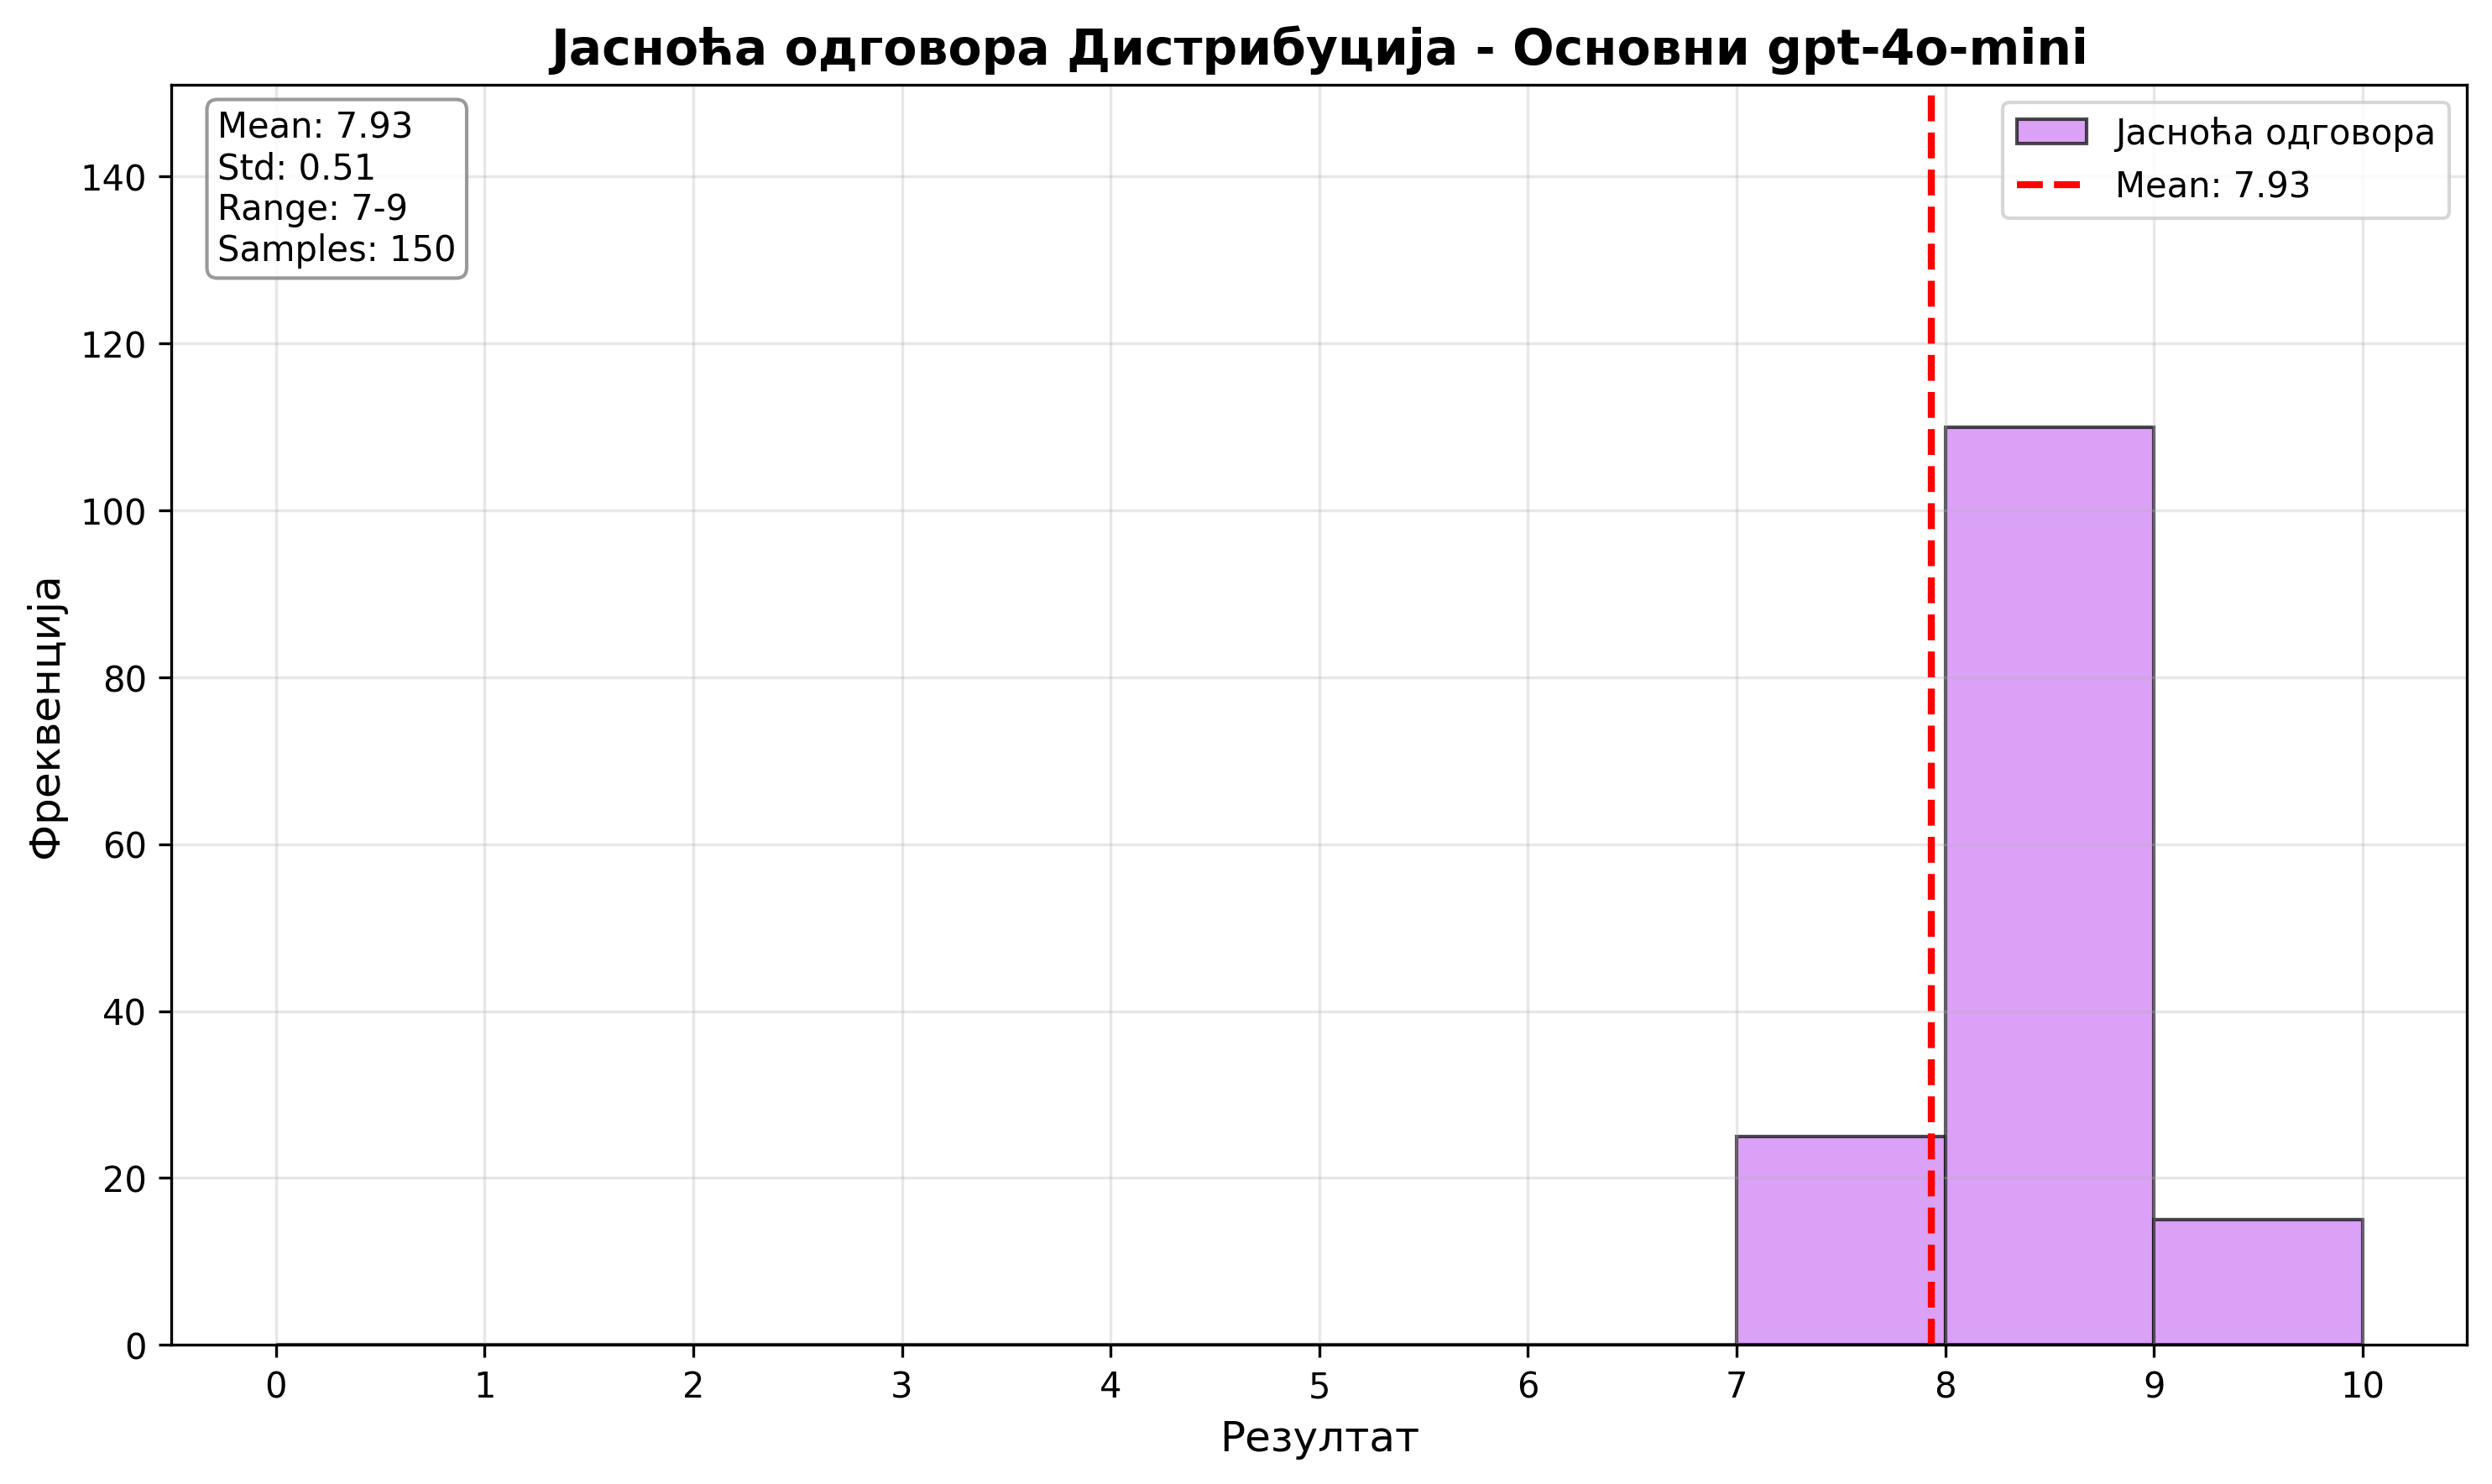
\includegraphics[width=0.8\textwidth]{images/osnovni/criteria_analysis_clarity_histogram.png}
    
    \vspace{0.5cm}
    
    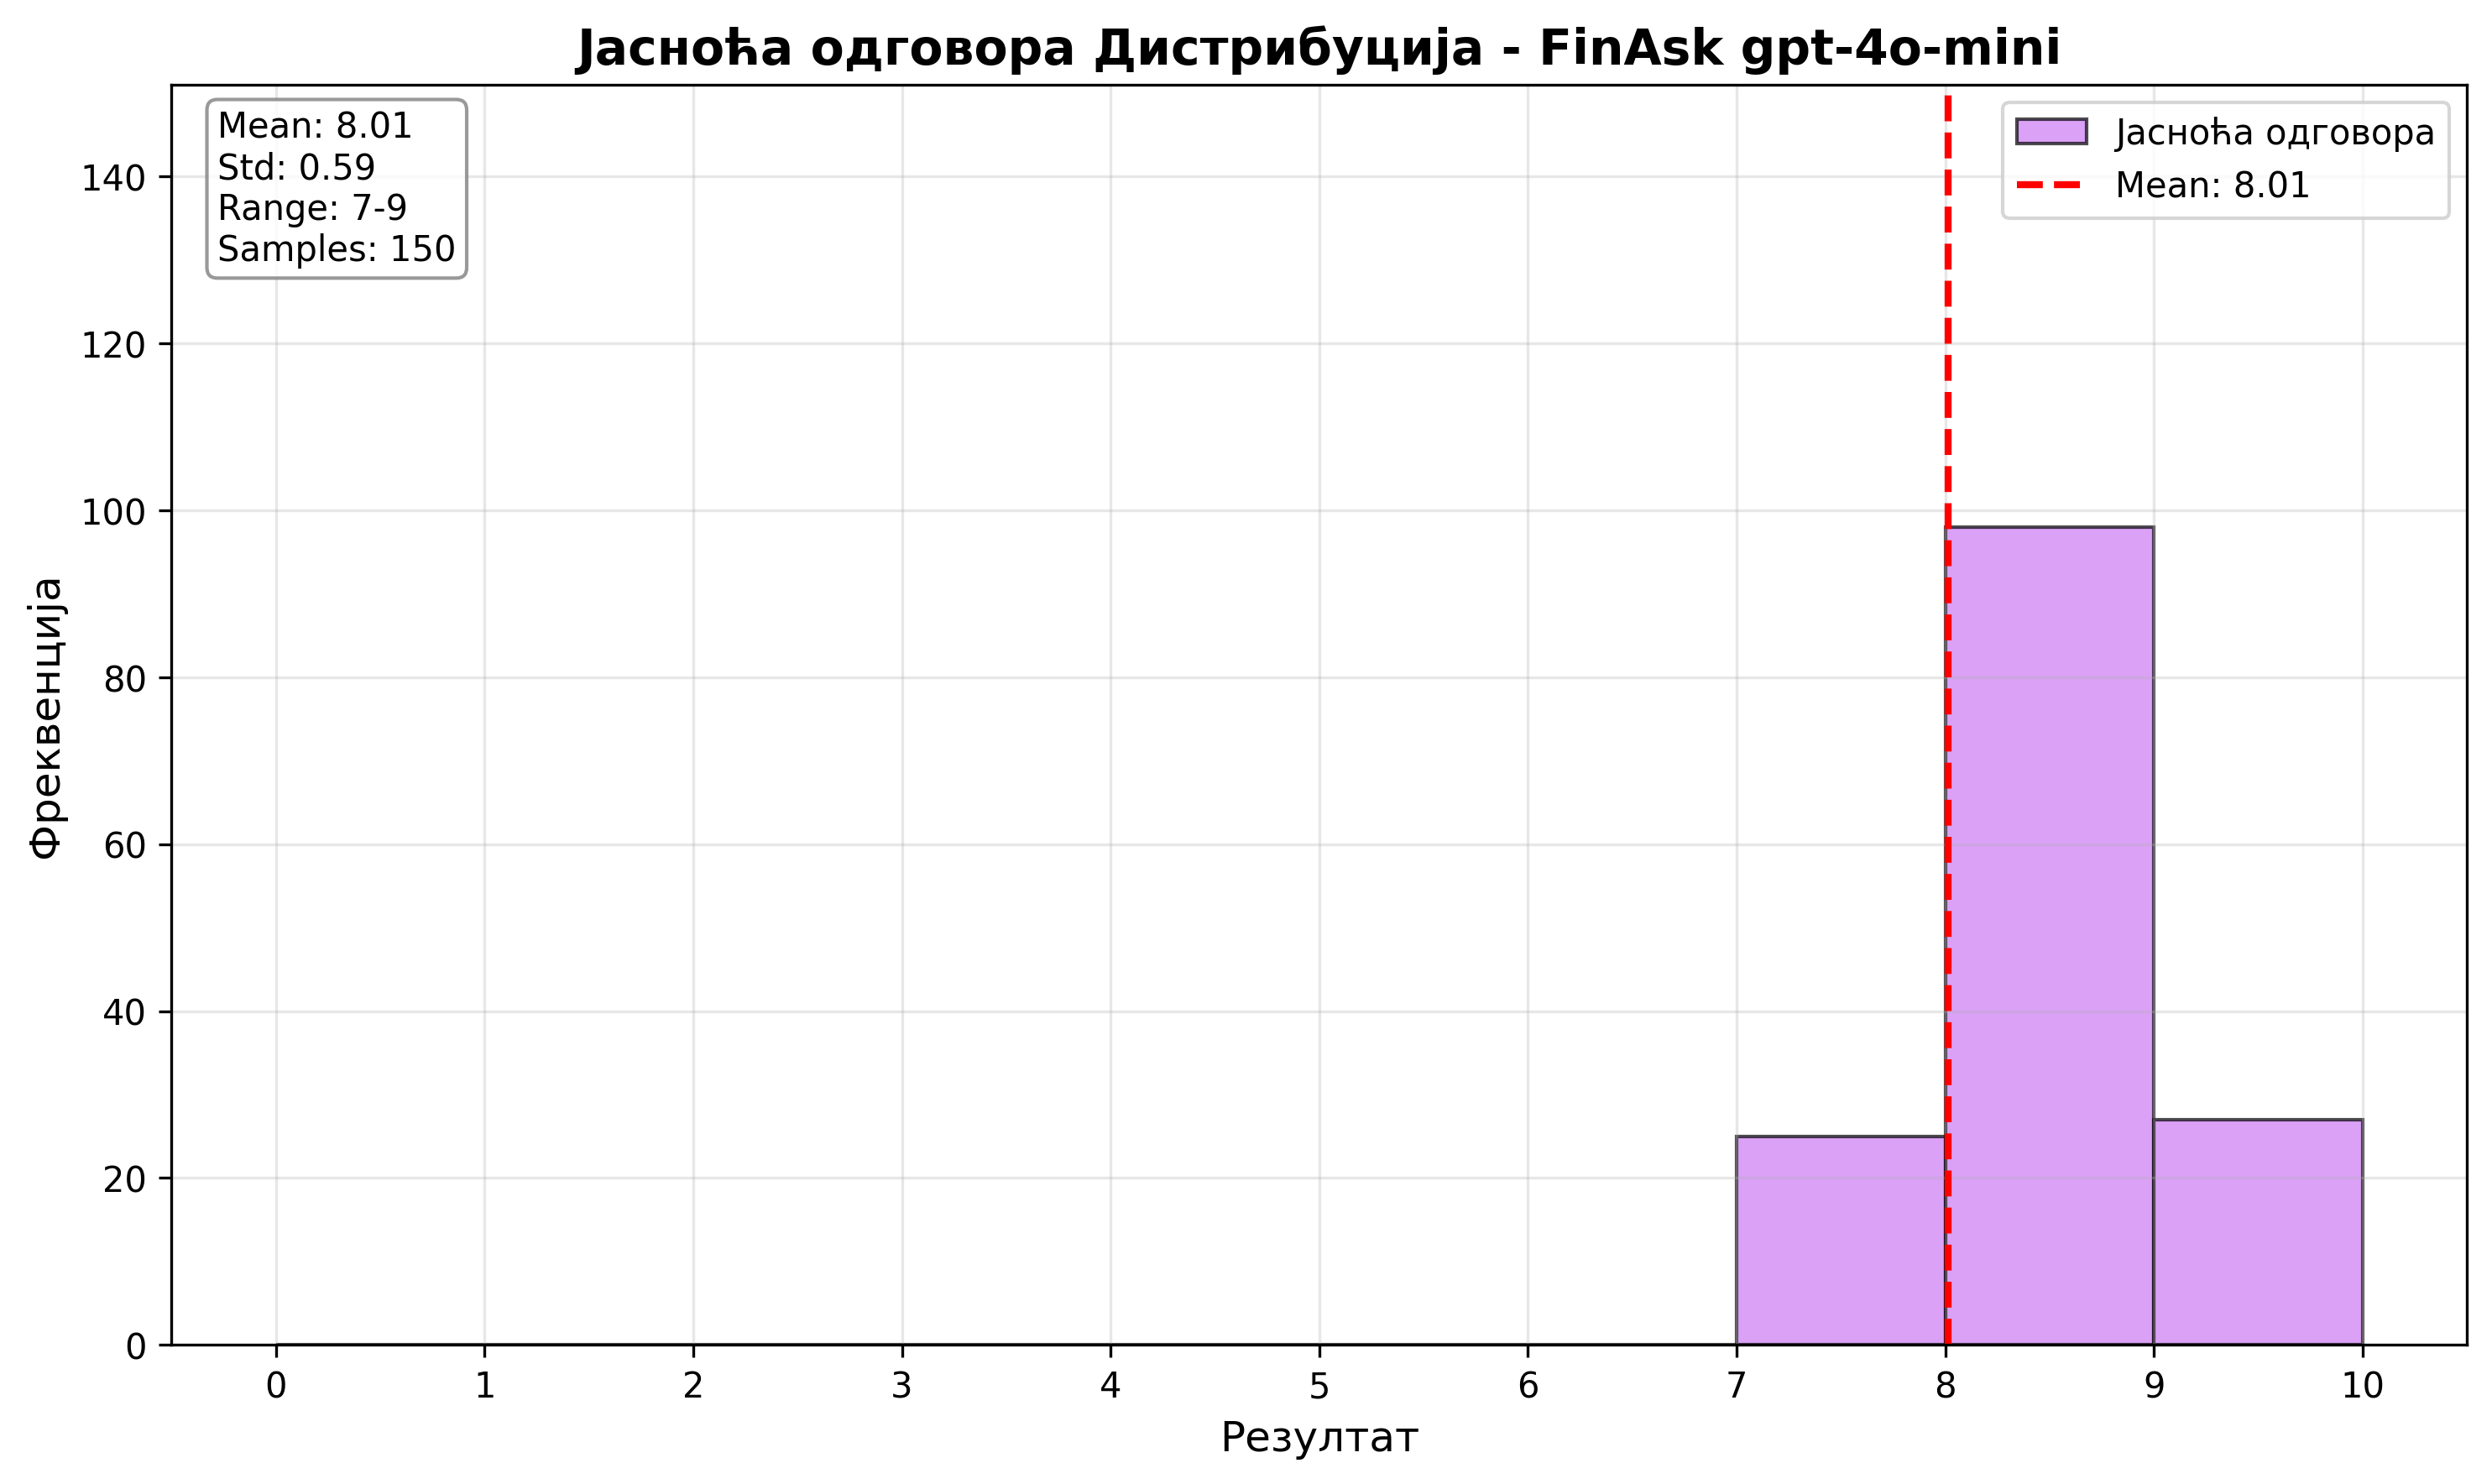
\includegraphics[width=0.8\textwidth]{images/FinAsk/criteria_analysis_clarity_histogram.png}
    \caption{Хистограм анализе критеријума јасноће - горе: основни модел, доле: FinAsk модел}
    \label{fig:comparison_clarity}
\end{figure}

\subsection{Анализа критеријума потпуности одговора}

Комплетност одговора са средњим скором од 6.41 и стандардном девијацијом од 1.03 указује на релативно конзистентну перформансу у овом домену, што сугерише да архитектура система подржава систематичан приступ структурирању одговора. У поређењу са основним моделом, FinAsk модел показује благо погоршање у просечним оценама, што указује на негативан утицај прилагођавања промпта на способност пружања обухватних анализа. Приказ поређења хистограма налази се на слици \ref{fig:comparison_completeness}.

\begin{figure}[h]
    \centering
    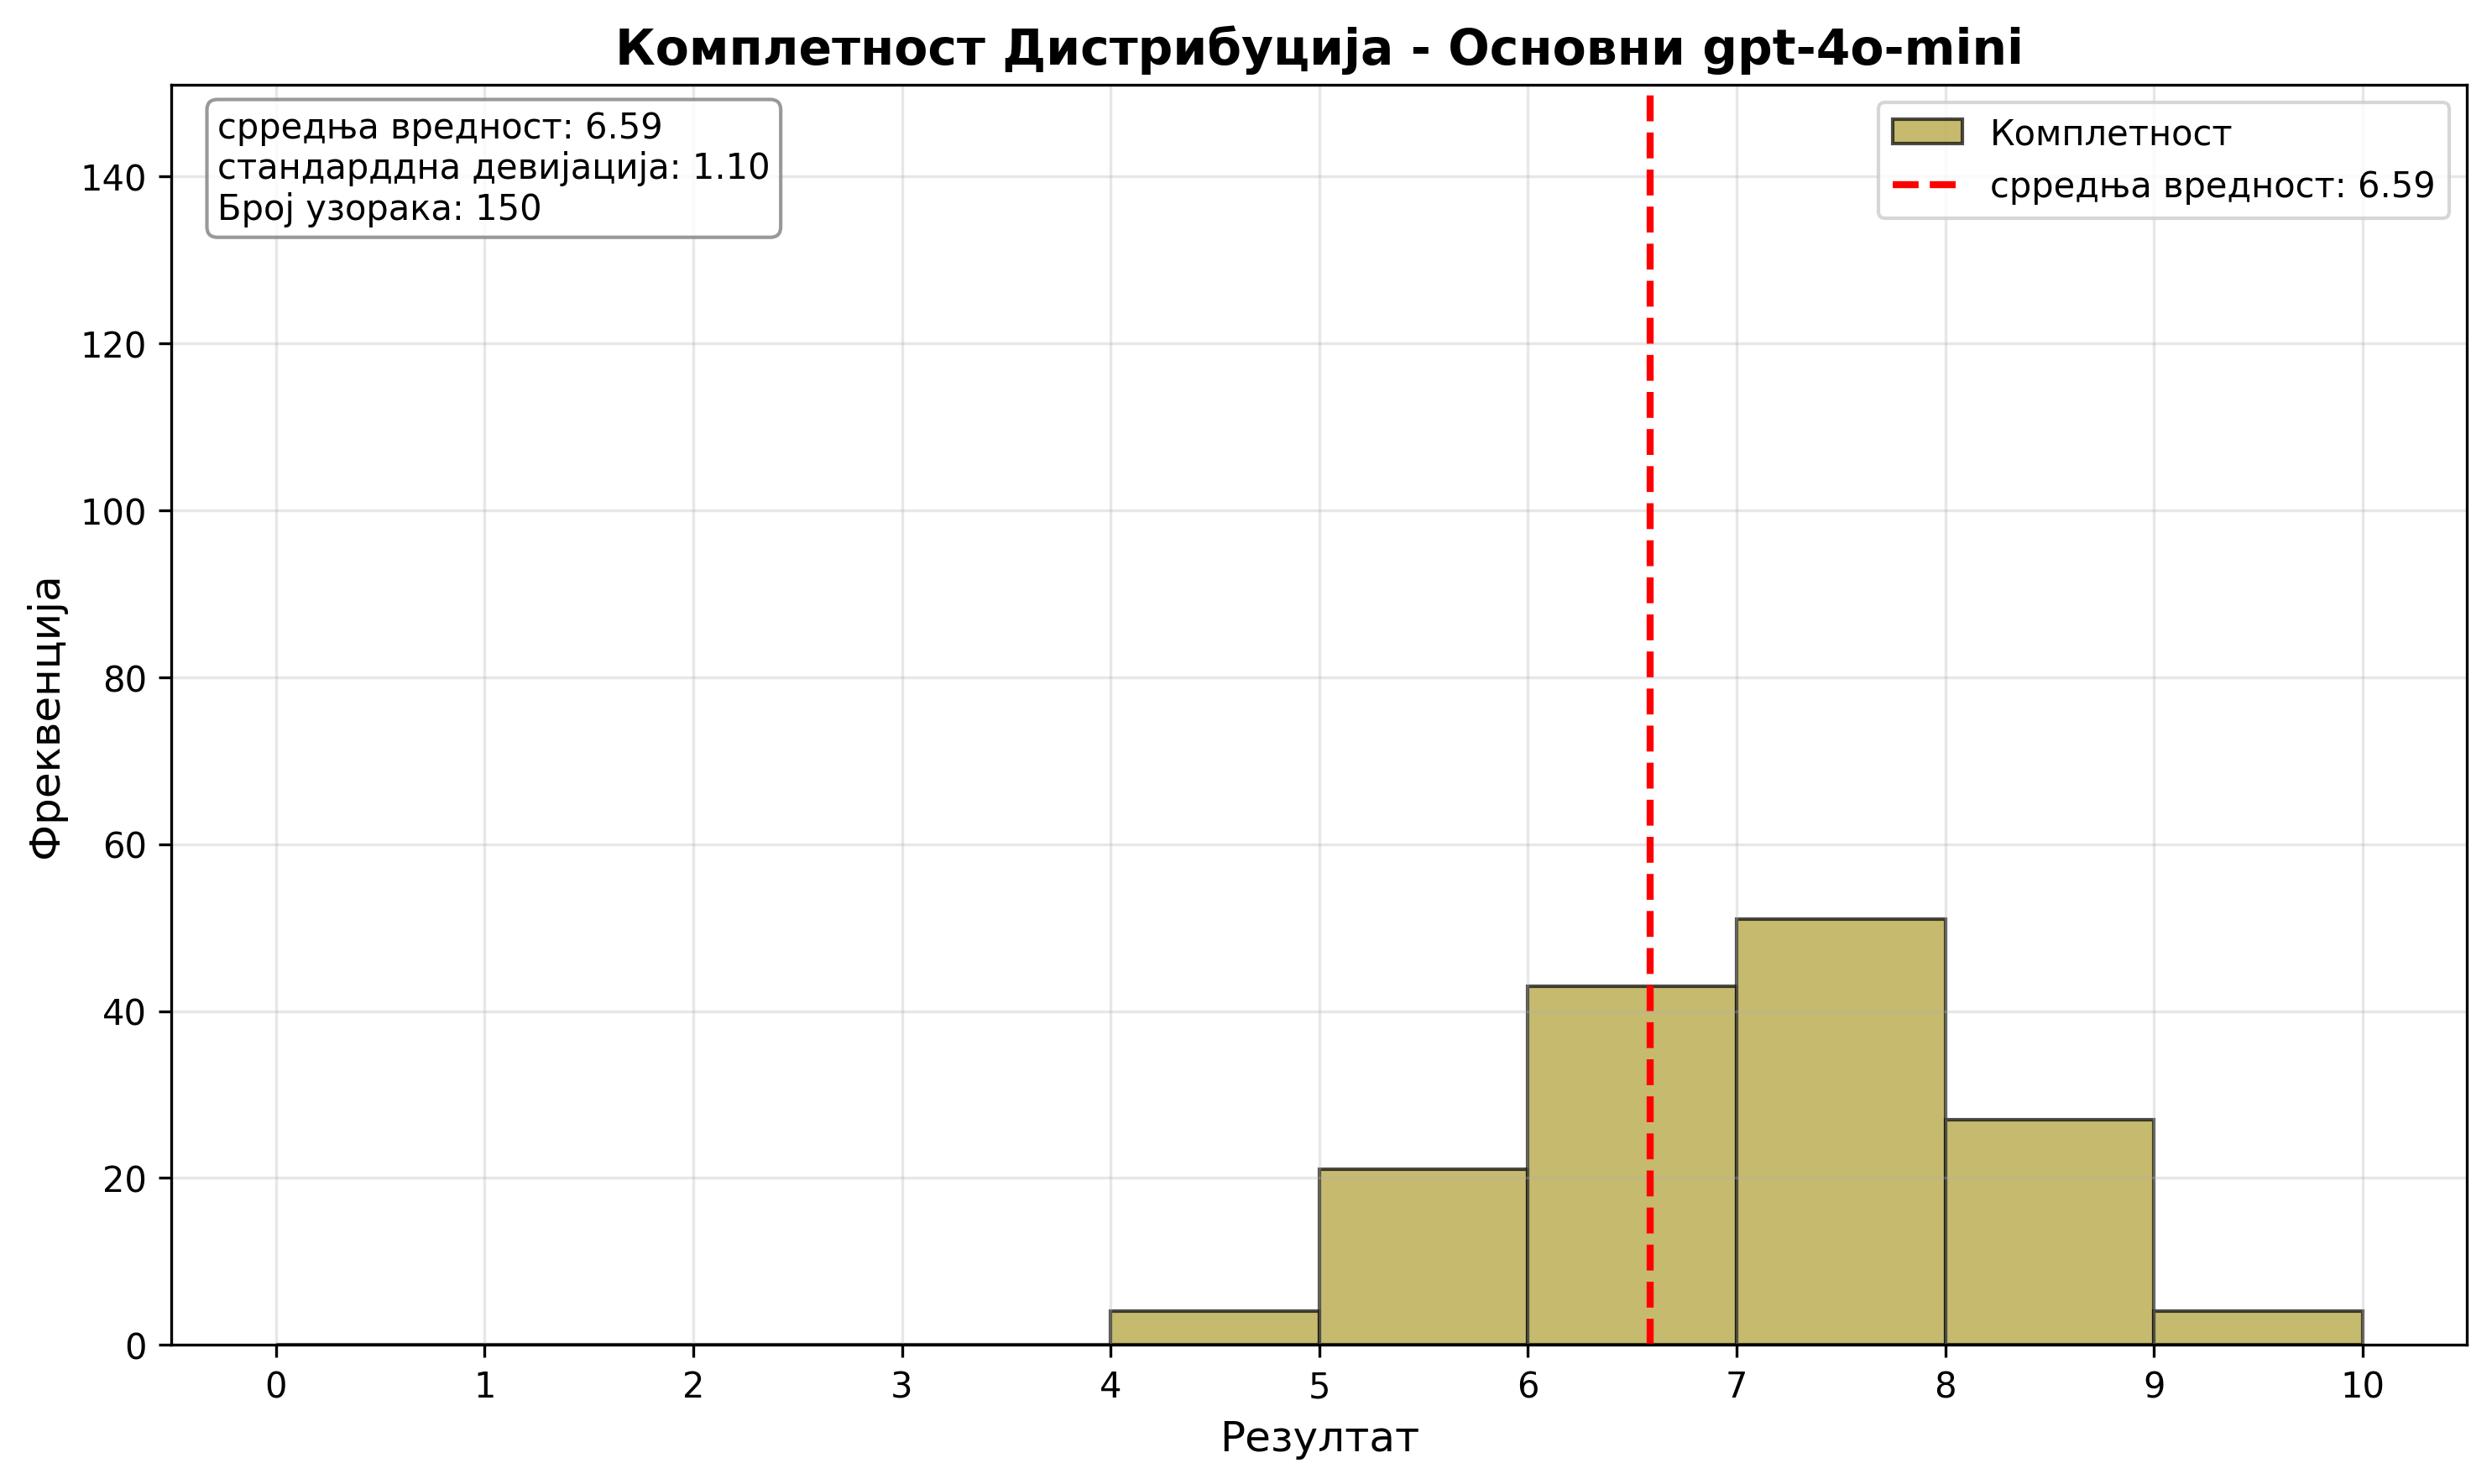
\includegraphics[width=0.8\textwidth]{images/osnovni/criteria_analysis_completeness_histogram.png}
    
    \vspace{0.5cm}
    
    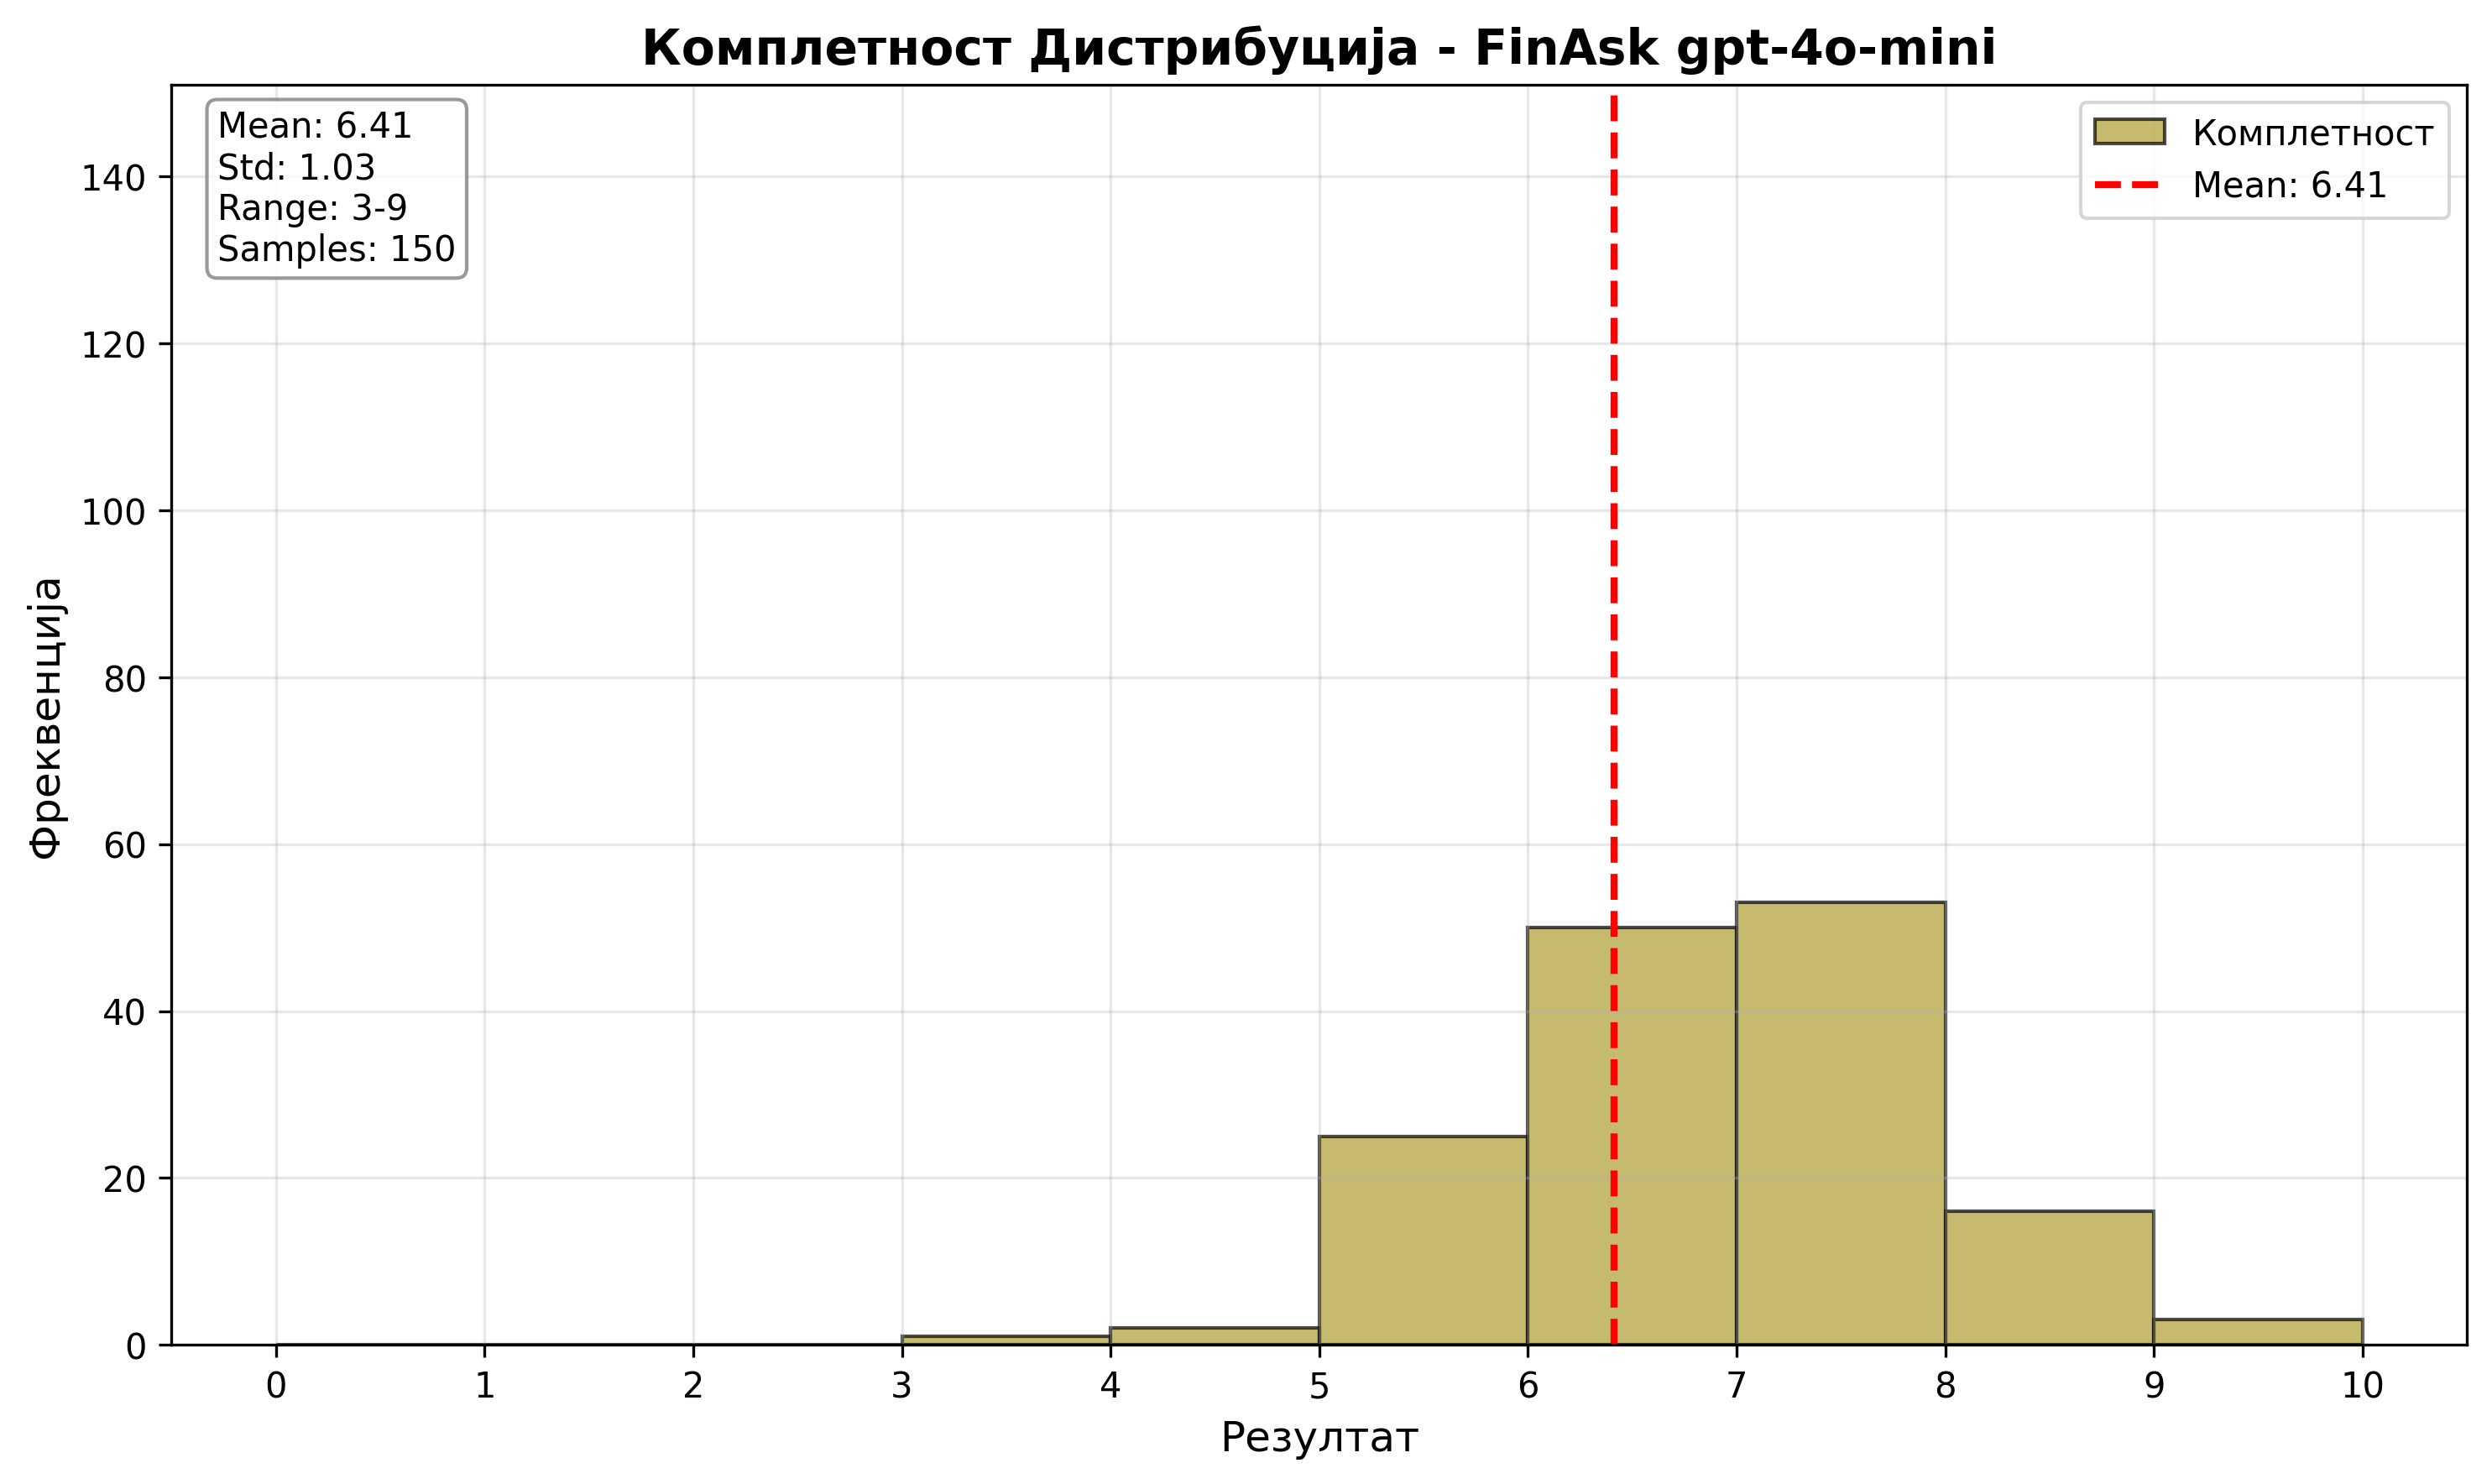
\includegraphics[width=0.8\textwidth]{images/FinAsk/criteria_analysis_completeness_histogram.png}
    \caption{Хистограм анализе критеријума потпуности - горе: основни модел, доле: FinAsk модел}
    \label{fig:comparison_completeness}
\end{figure}

\subsection{Анализа критеријума тачности}

Фактуална исправност са просечним скором од 5.09 и стандардном девијацијом од 1.26 представља умерен ниво тачности који сугерише да систем успева да идентификује и репродукује релевантне финансијске информације у приближно половини случајева. Ова метрика је кључна за практичну примену система јер директно утиче на поверење корисника и употребљивост у реалним сценаријима финансијског саветовања. Релативно висока варијабилност указује на недоследност у приступу обради различитих типова упита, што може бити последица ограничења у основном језичком моделу или недовољне оптимизације промпт инжењеринга. У односу на основни модел приметно је велико побољшање што говори да основни модел нема информације које су потребне за тачан одговор, а FinAsk модел их успешно проналази. Додатно, ово показује способност агент асудије да распознаје и награди тачне одговоре. Приказ поређења хистограма налази се на слици \ref{fig:comparison_factual}.

\begin{figure}[h]
    \centering
    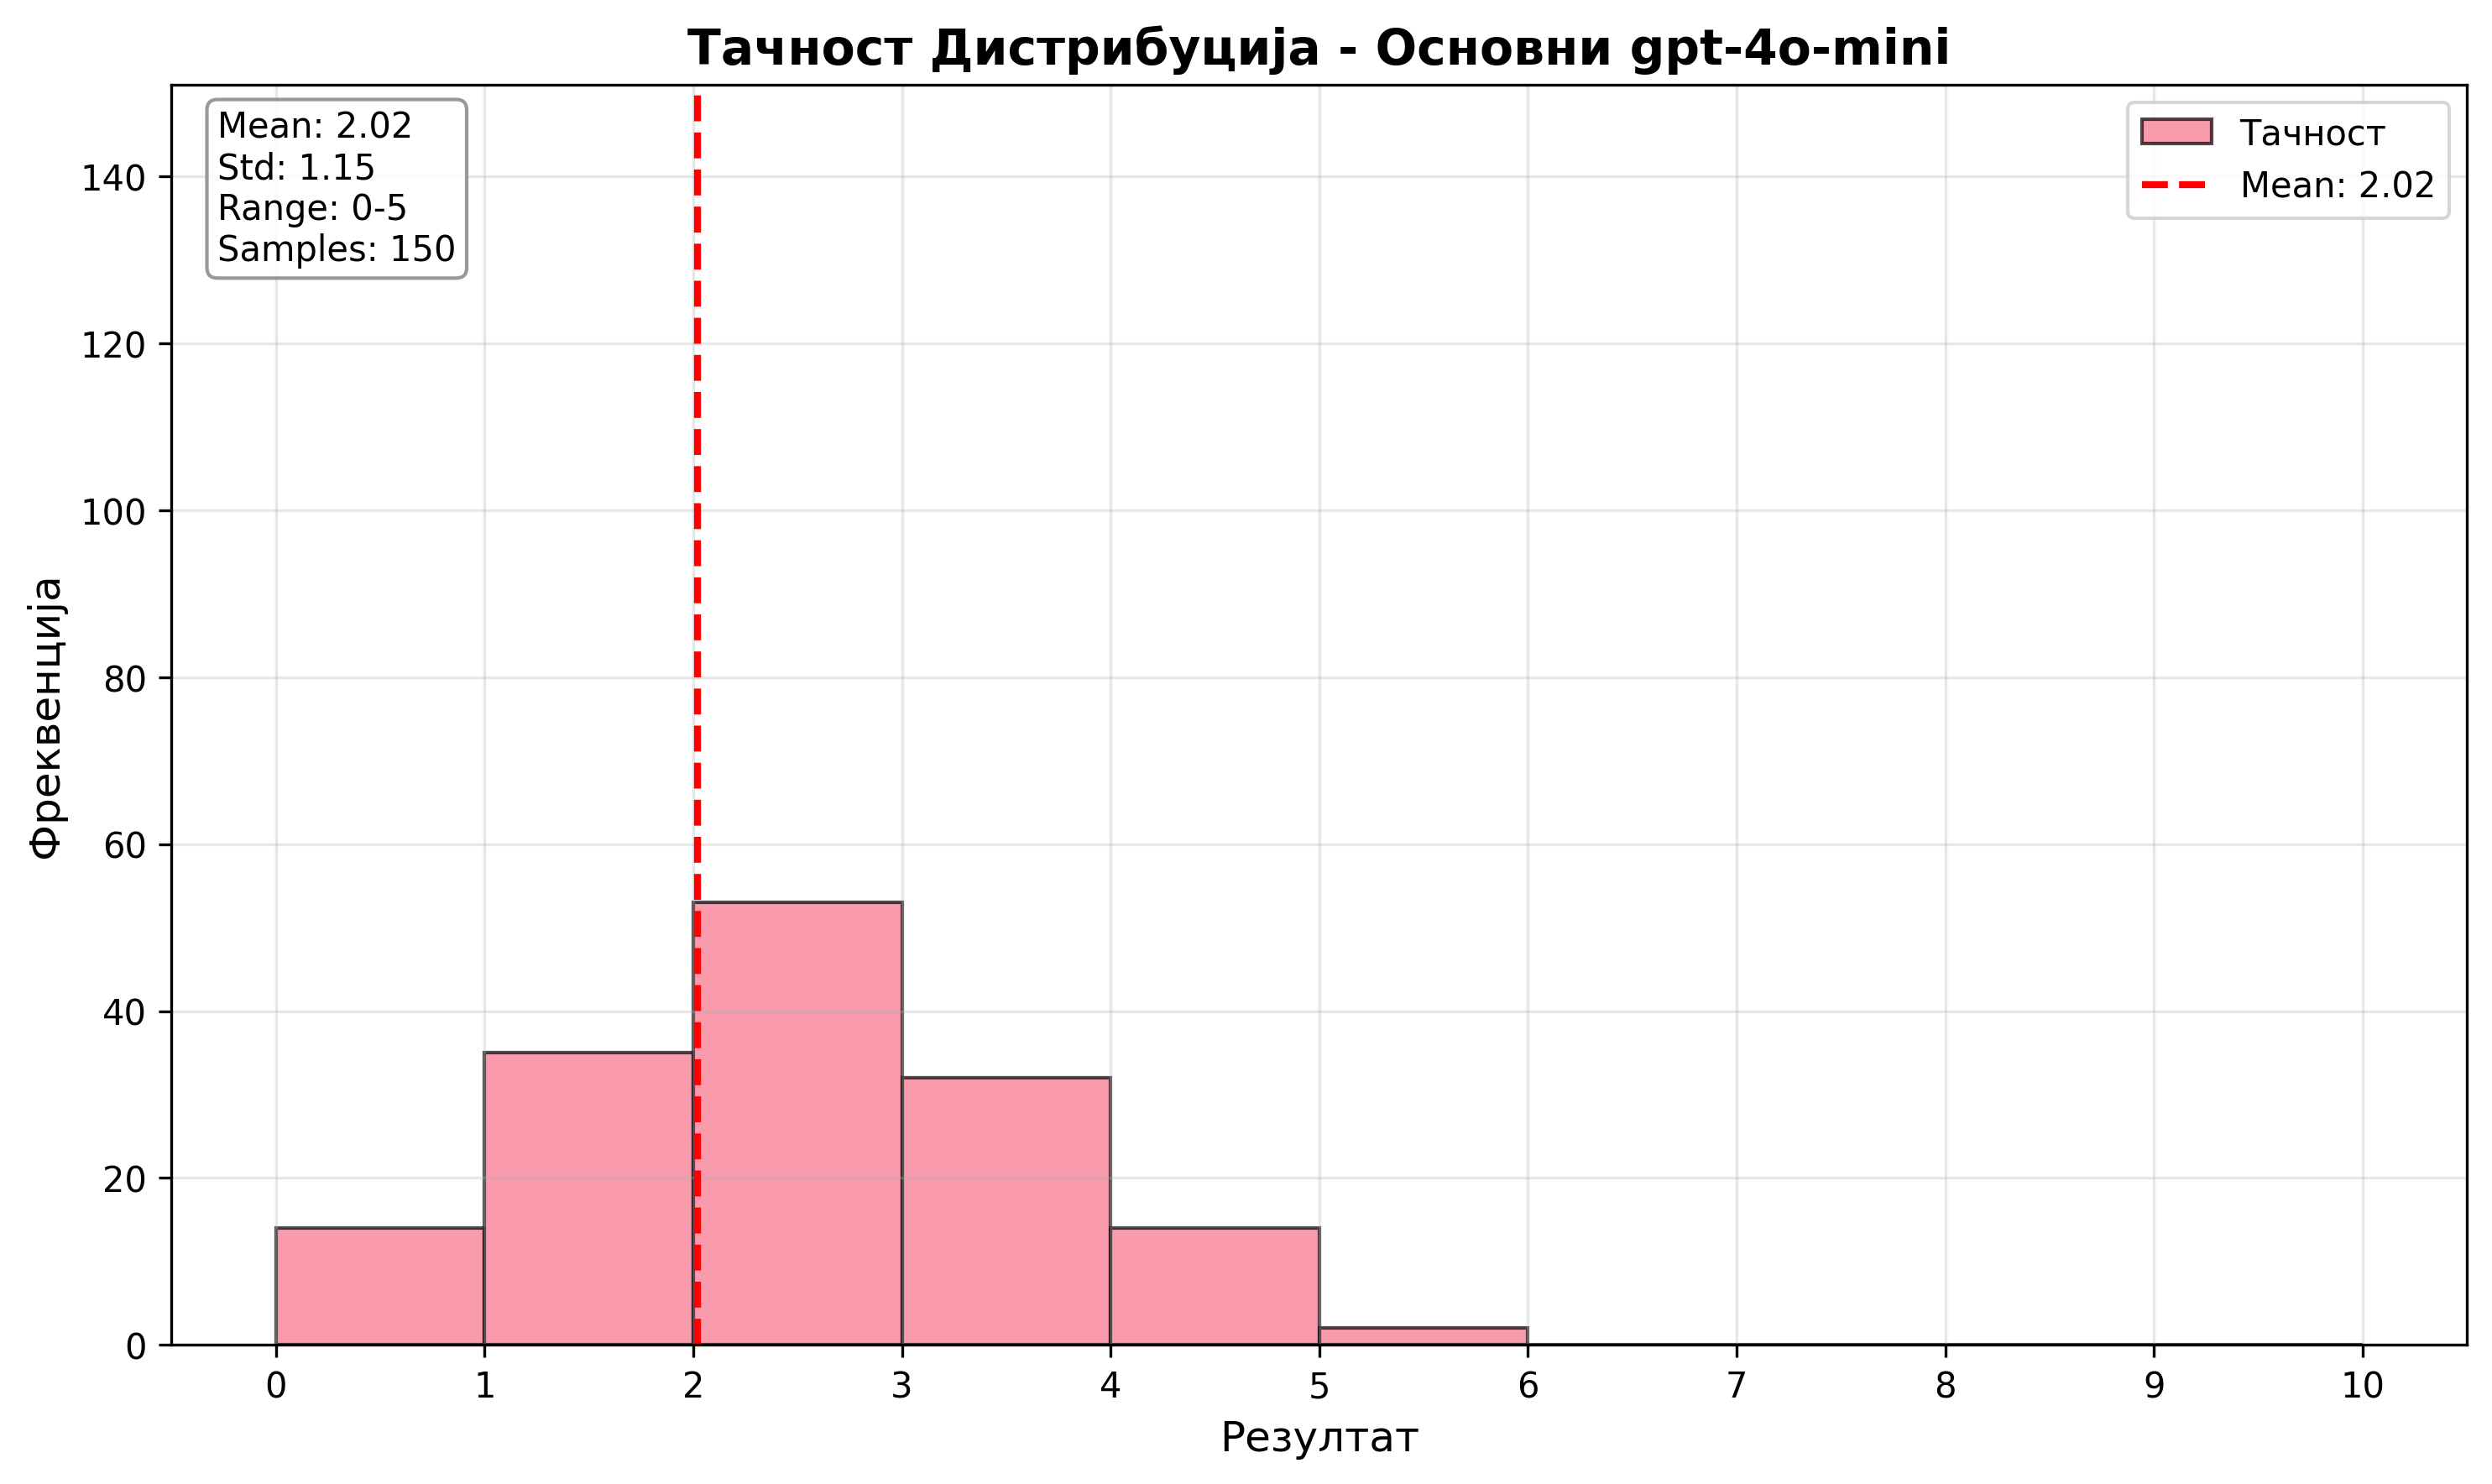
\includegraphics[width=0.8\textwidth]{images/osnovni/criteria_analysis_factual_correctness_histogram.png}
    
    \vspace{0.5cm}
    
    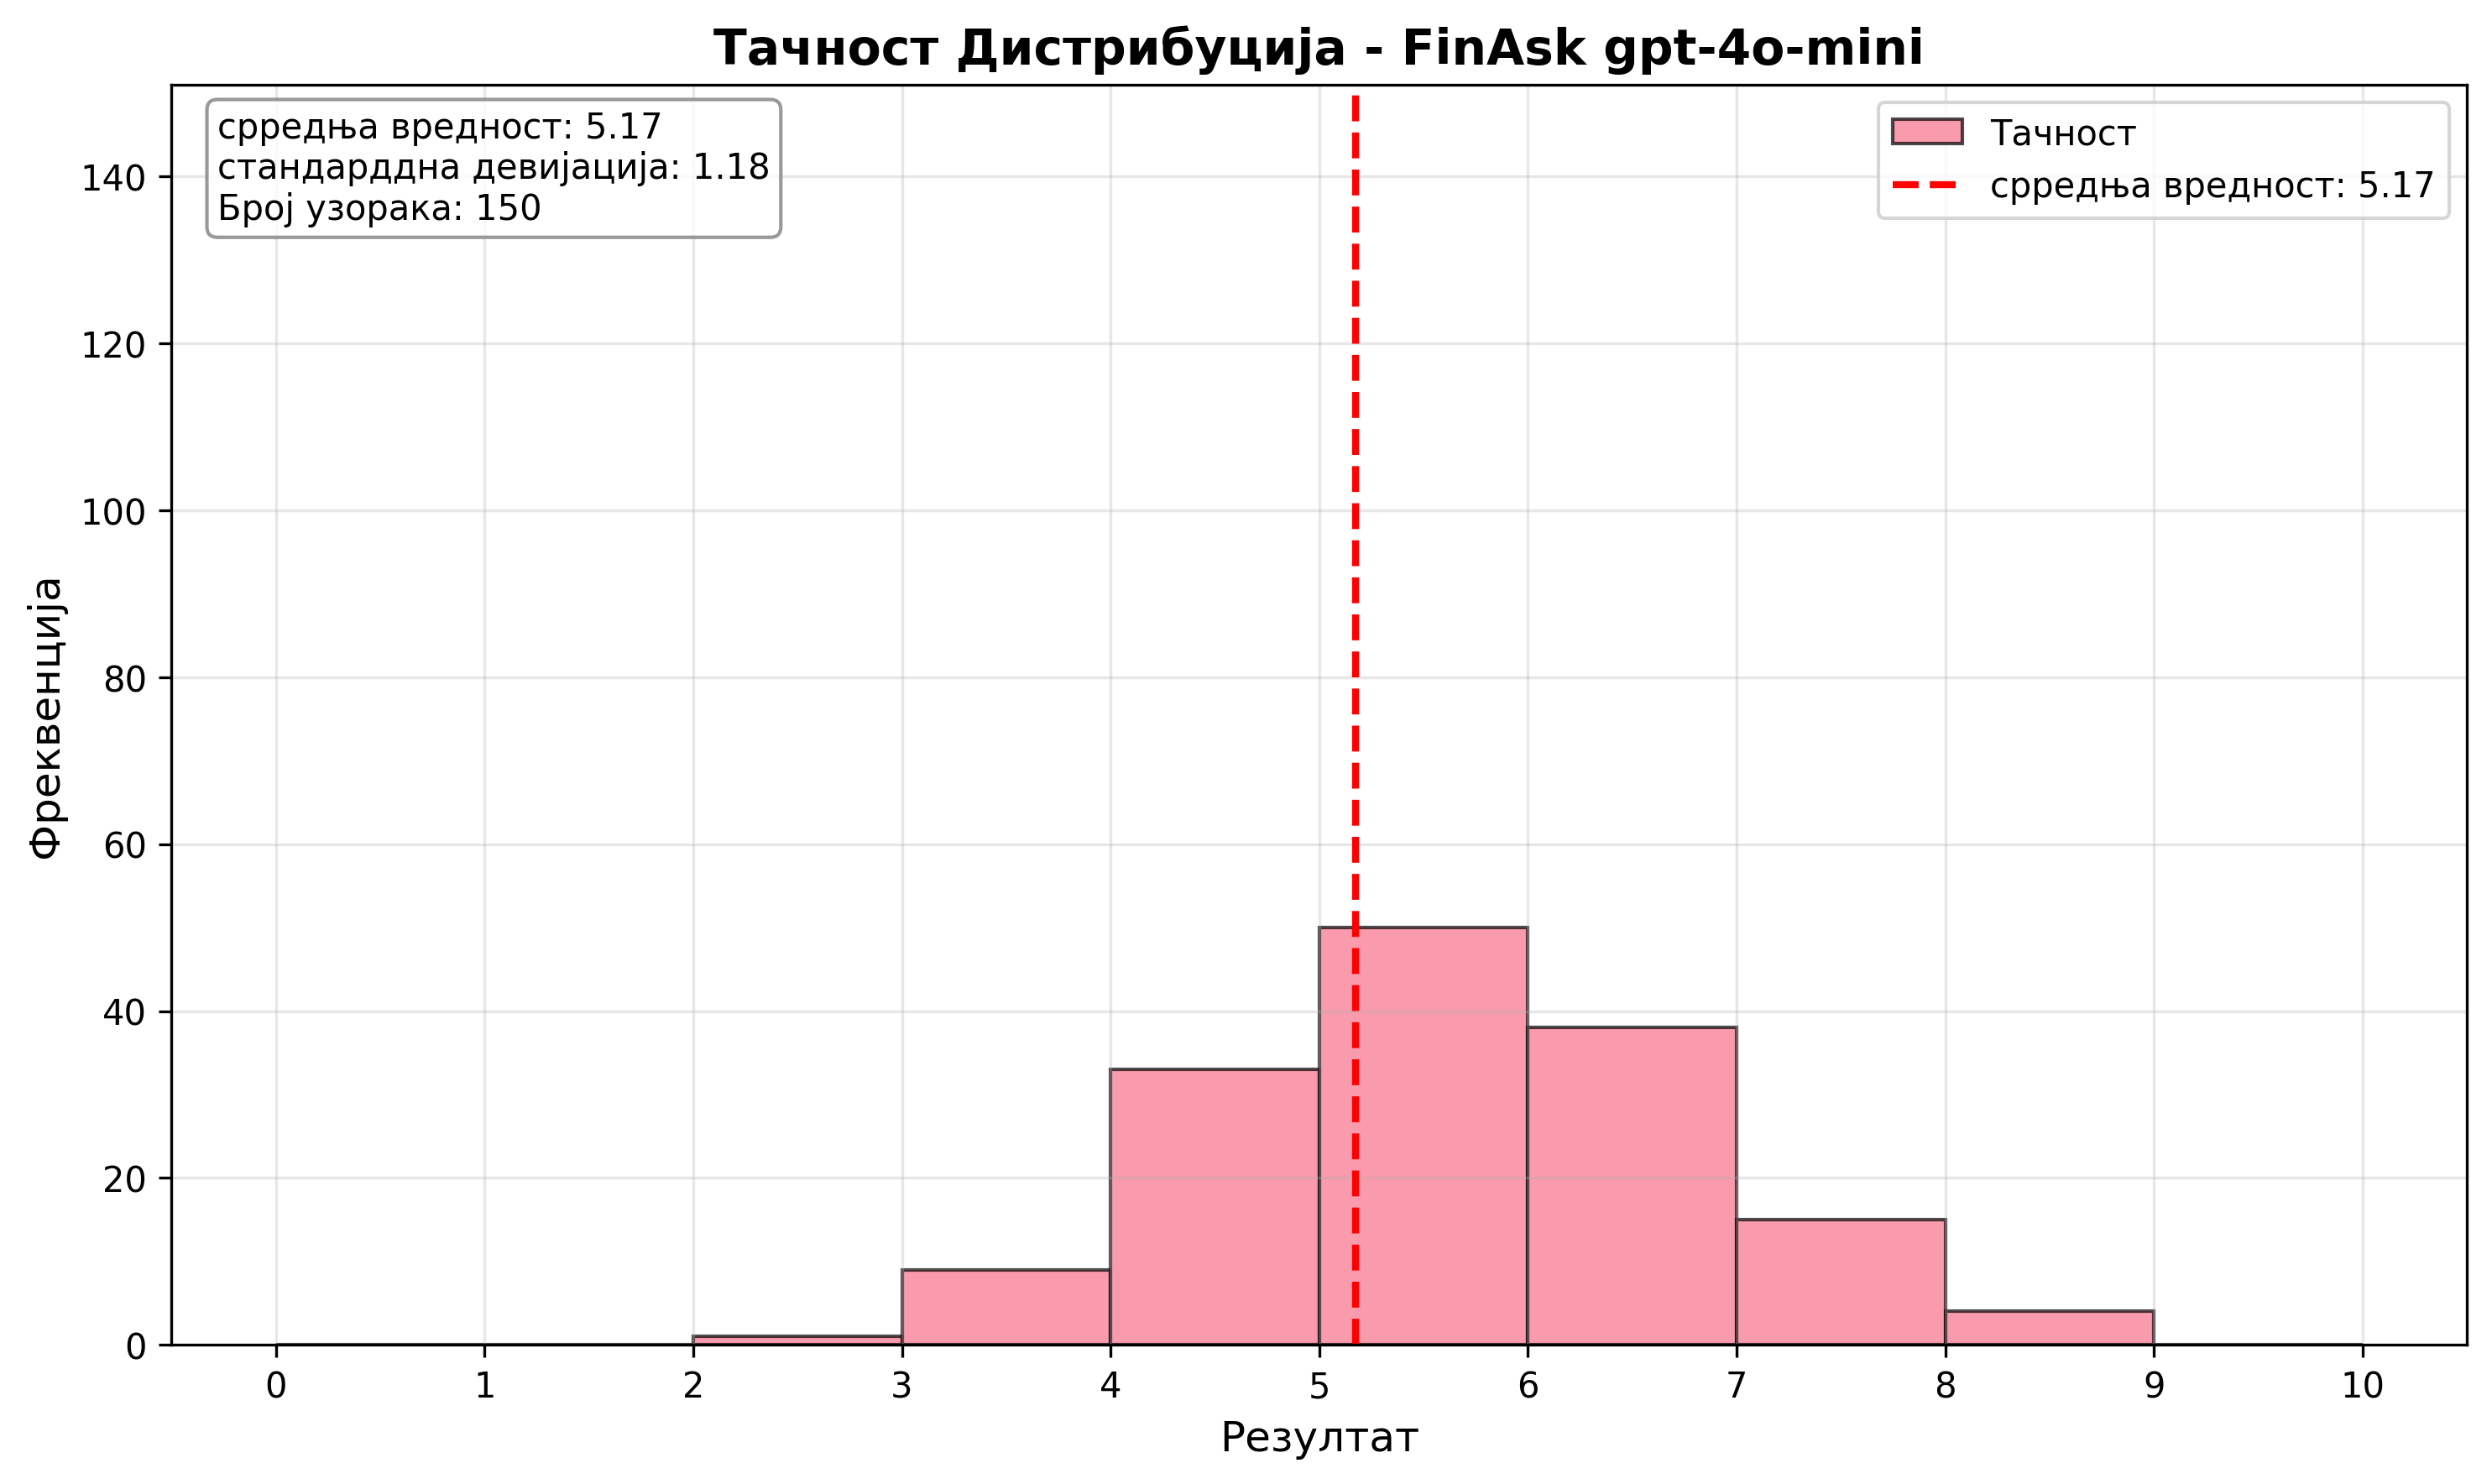
\includegraphics[width=0.8\textwidth]{images/FinAsk/criteria_analysis_factual_correctness_histogram.png}
    \caption{Хистограм анализе критеријума фактичке тачности - горе: основни модел, доле: FinAsk модел}
    \label{fig:comparison_factual}
\end{figure}

\subsection{Анализа критеријума финансијског резоновања}

К Финансијско резоновање са скором од 7.97 представља један од најснажнијих аспеката система, указујући на способност извођења логичких закључака и примене финансијских принципа у анализи. Ова висока перформанса је посебно значајна јер одражава дубину разумевања финансијских концепата и способност њихове примене у различитим контекстовима. Међутим, разлика у скору између основног модела и FinAsk модела је минимална, што указује да прилагођавање промпта није донело значајно побољшање у овој области. Поставља се питање да ли прилагођавање промпта може утицати на дубину финансијског резоновања или су ове способности уграђене у основни језички модел. Приказ поређења хистограма налази се на слици \ref{fig:comparison_financial}.

\begin{figure}[h]
    \centering
    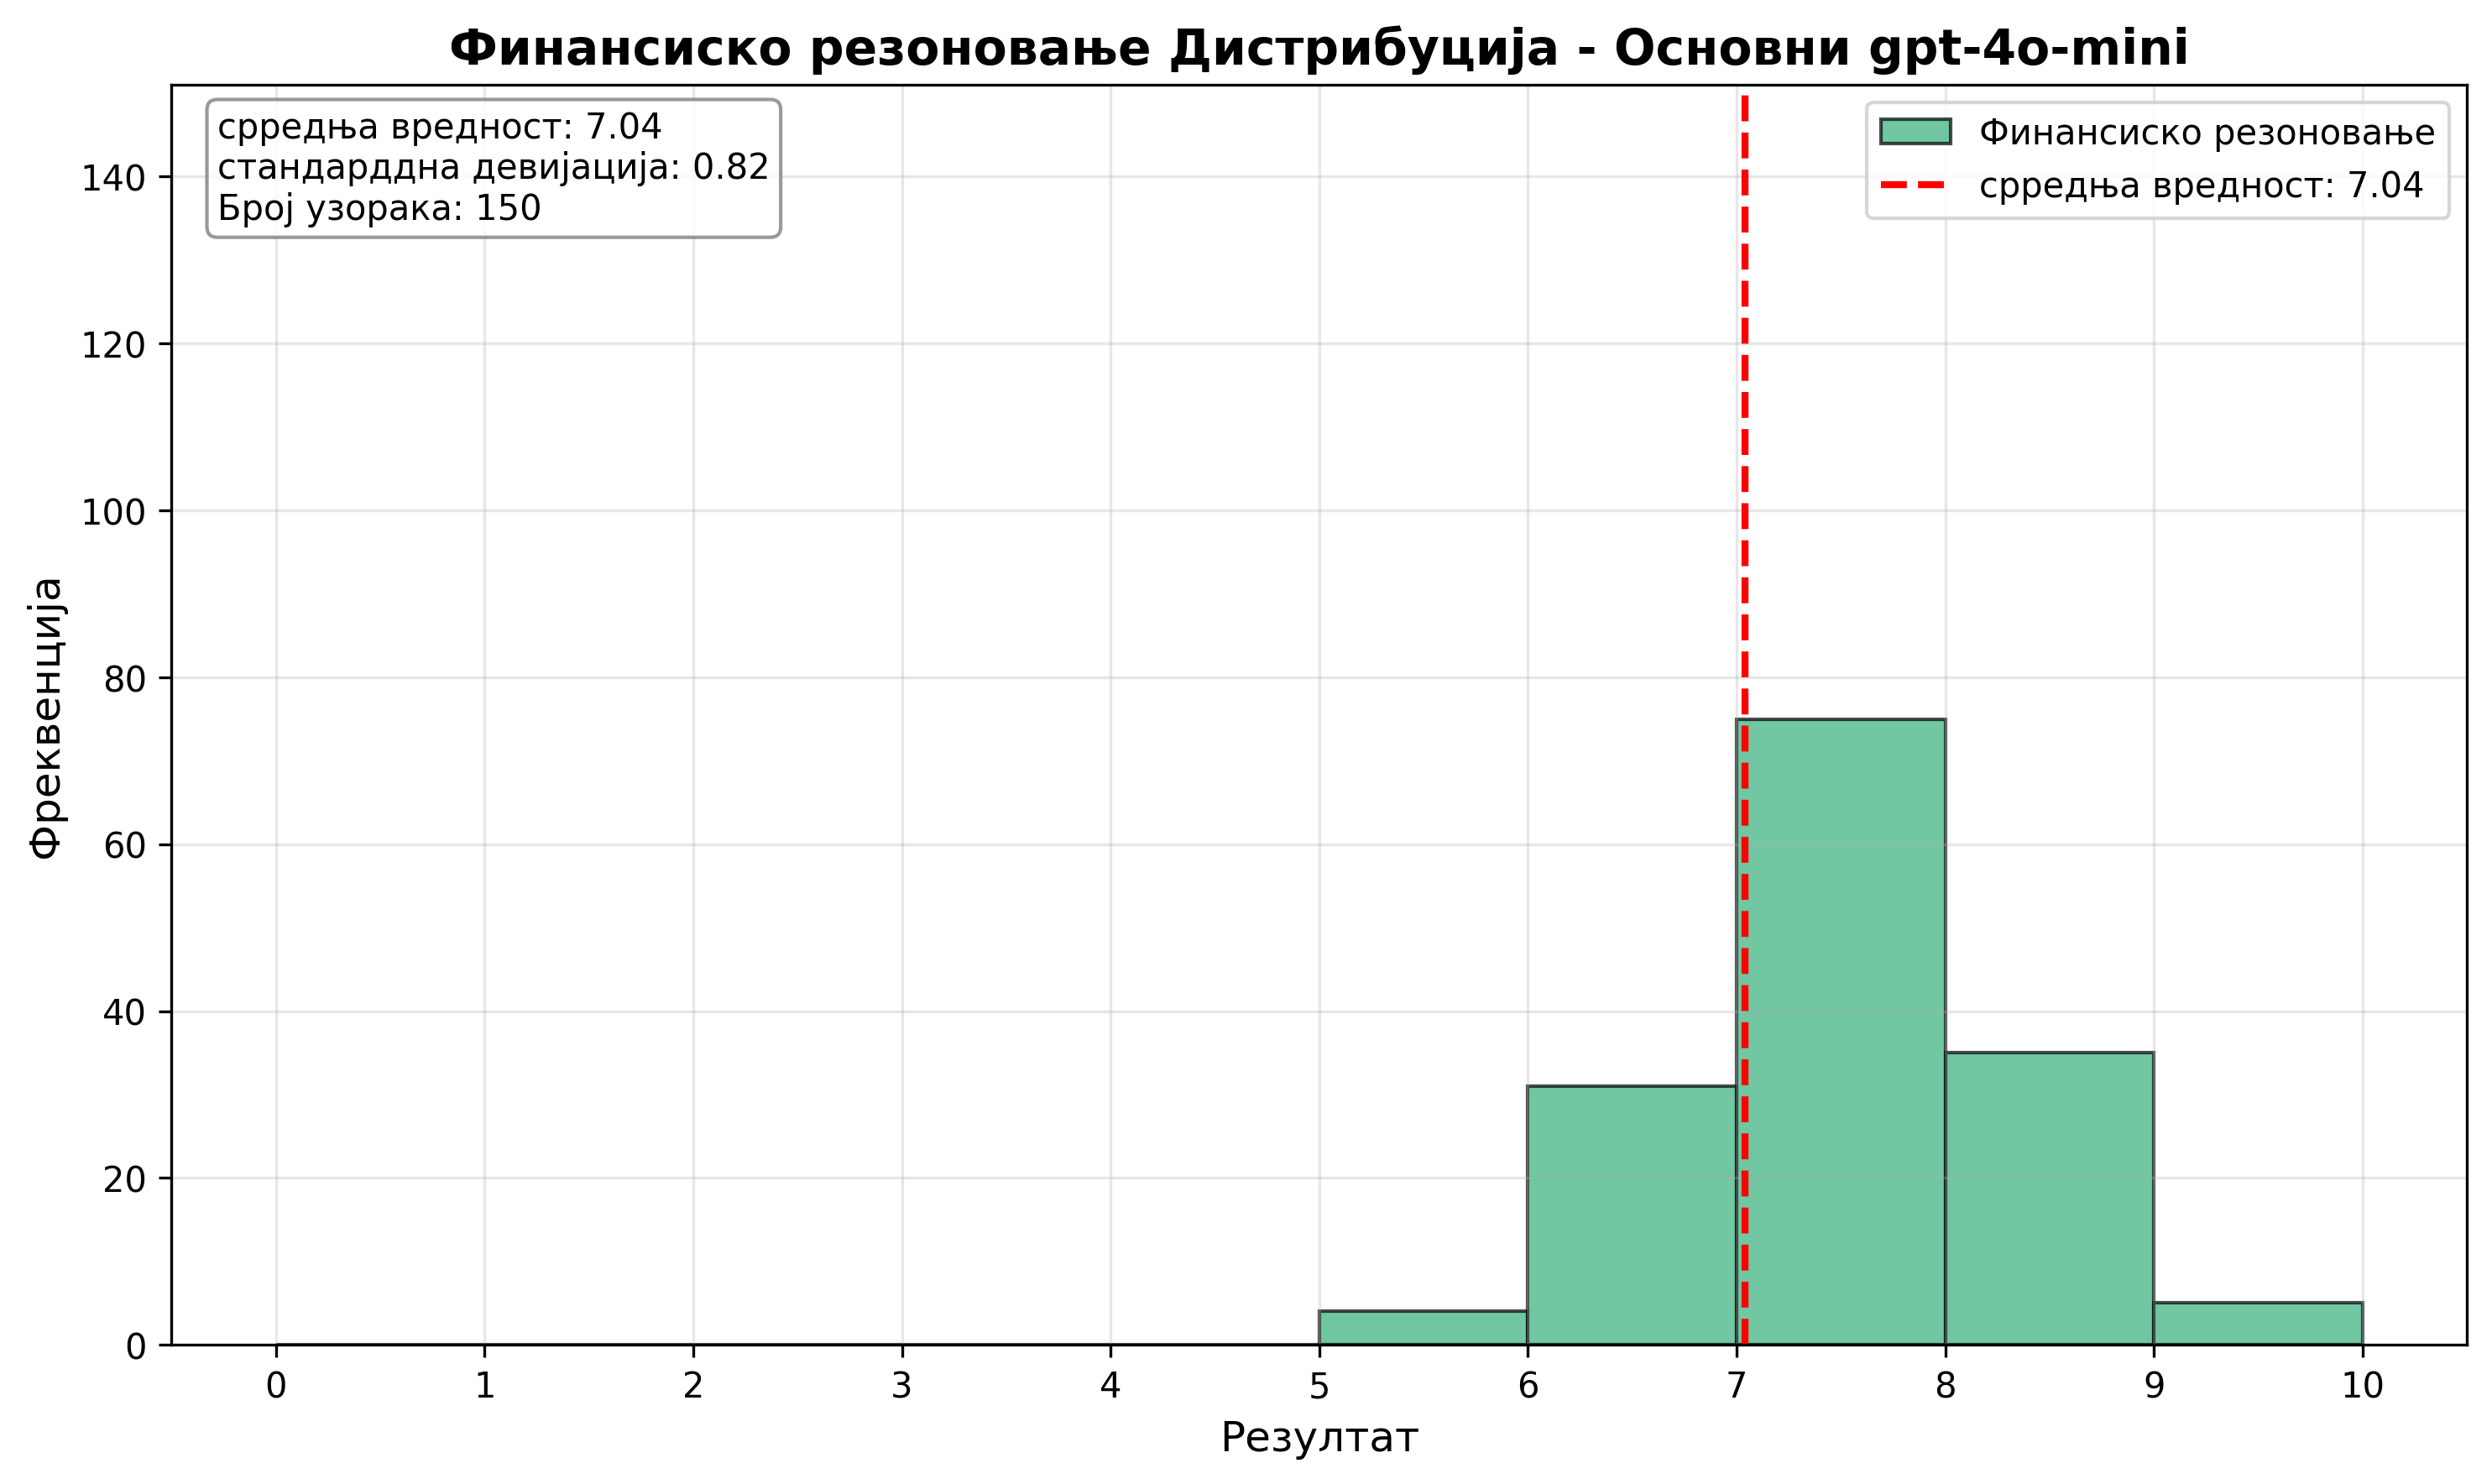
\includegraphics[width=0.8\textwidth]{images/osnovni/criteria_analysis_financial_reasoning_histogram.png}
    
    \vspace{0.5cm}
    
    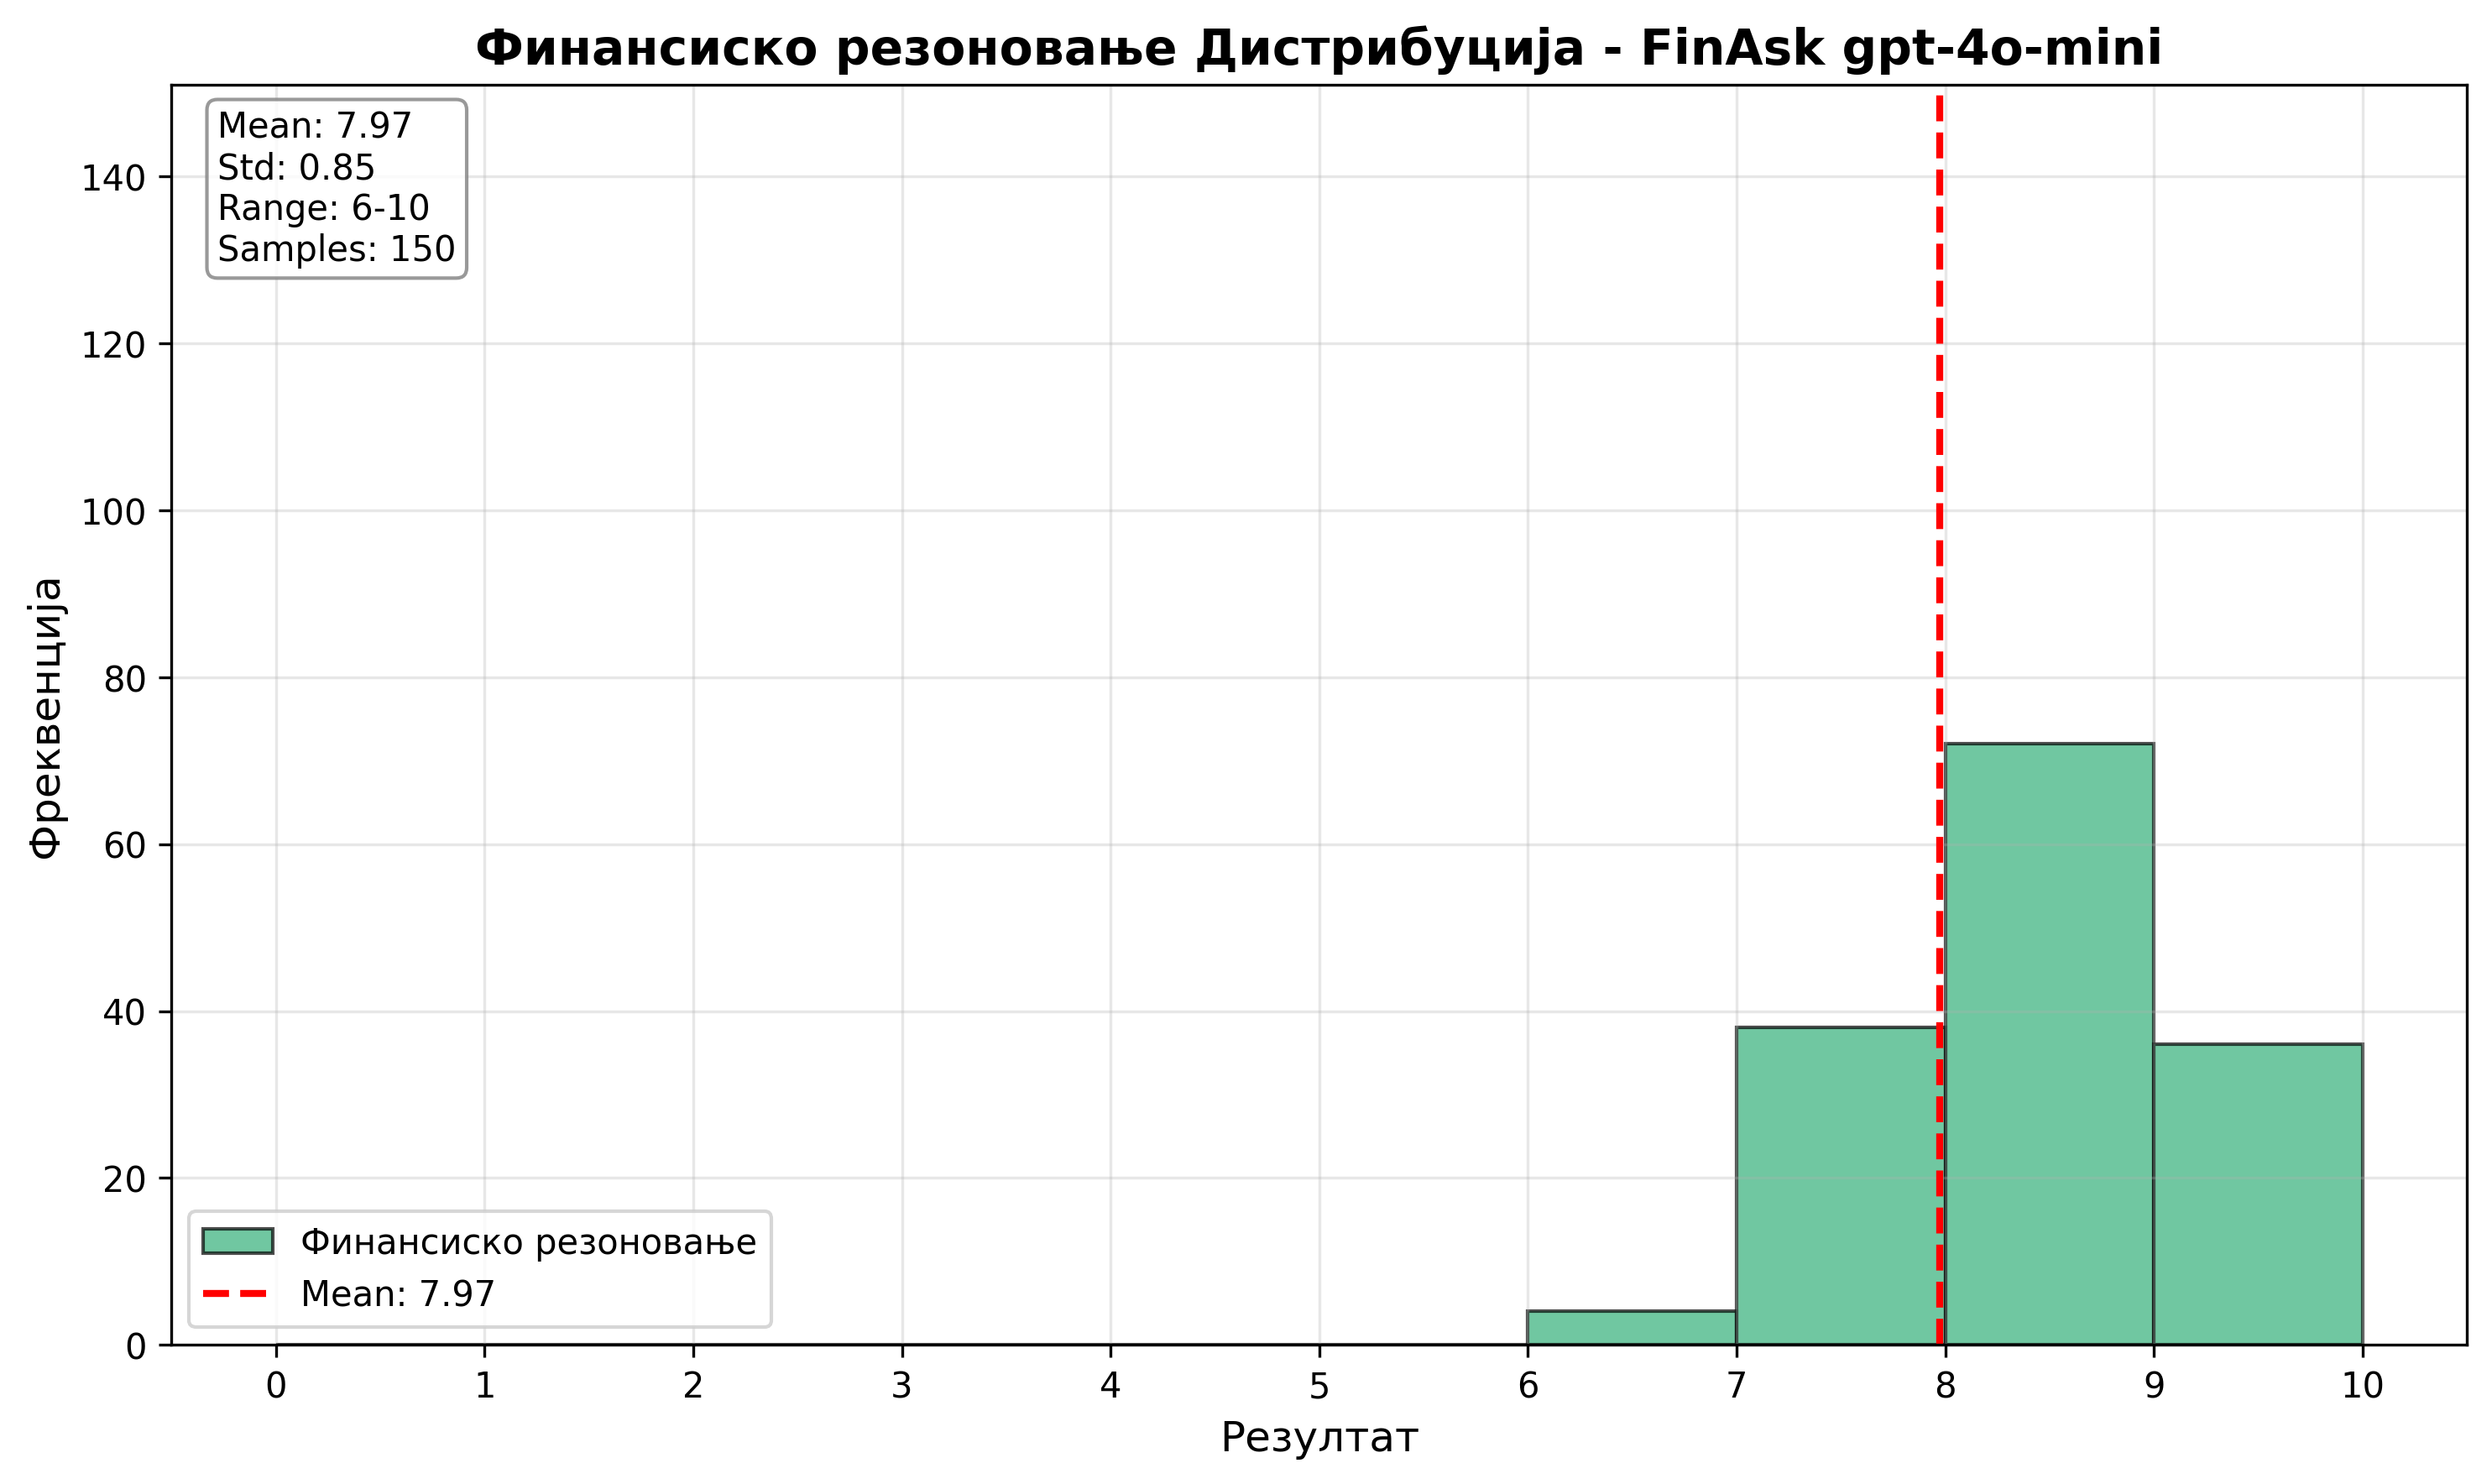
\includegraphics[width=0.8\textwidth]{images/FinAsk/criteria_analysis_financial_reasoning_histogram.png}
    \caption{Хистограм анализе критеријума финансијског резоновања - горе: основни модел, доле: FinAsk модел}
    \label{fig:comparison_financial}
\end{figure}

\begin{figure}[h]
    \centering
    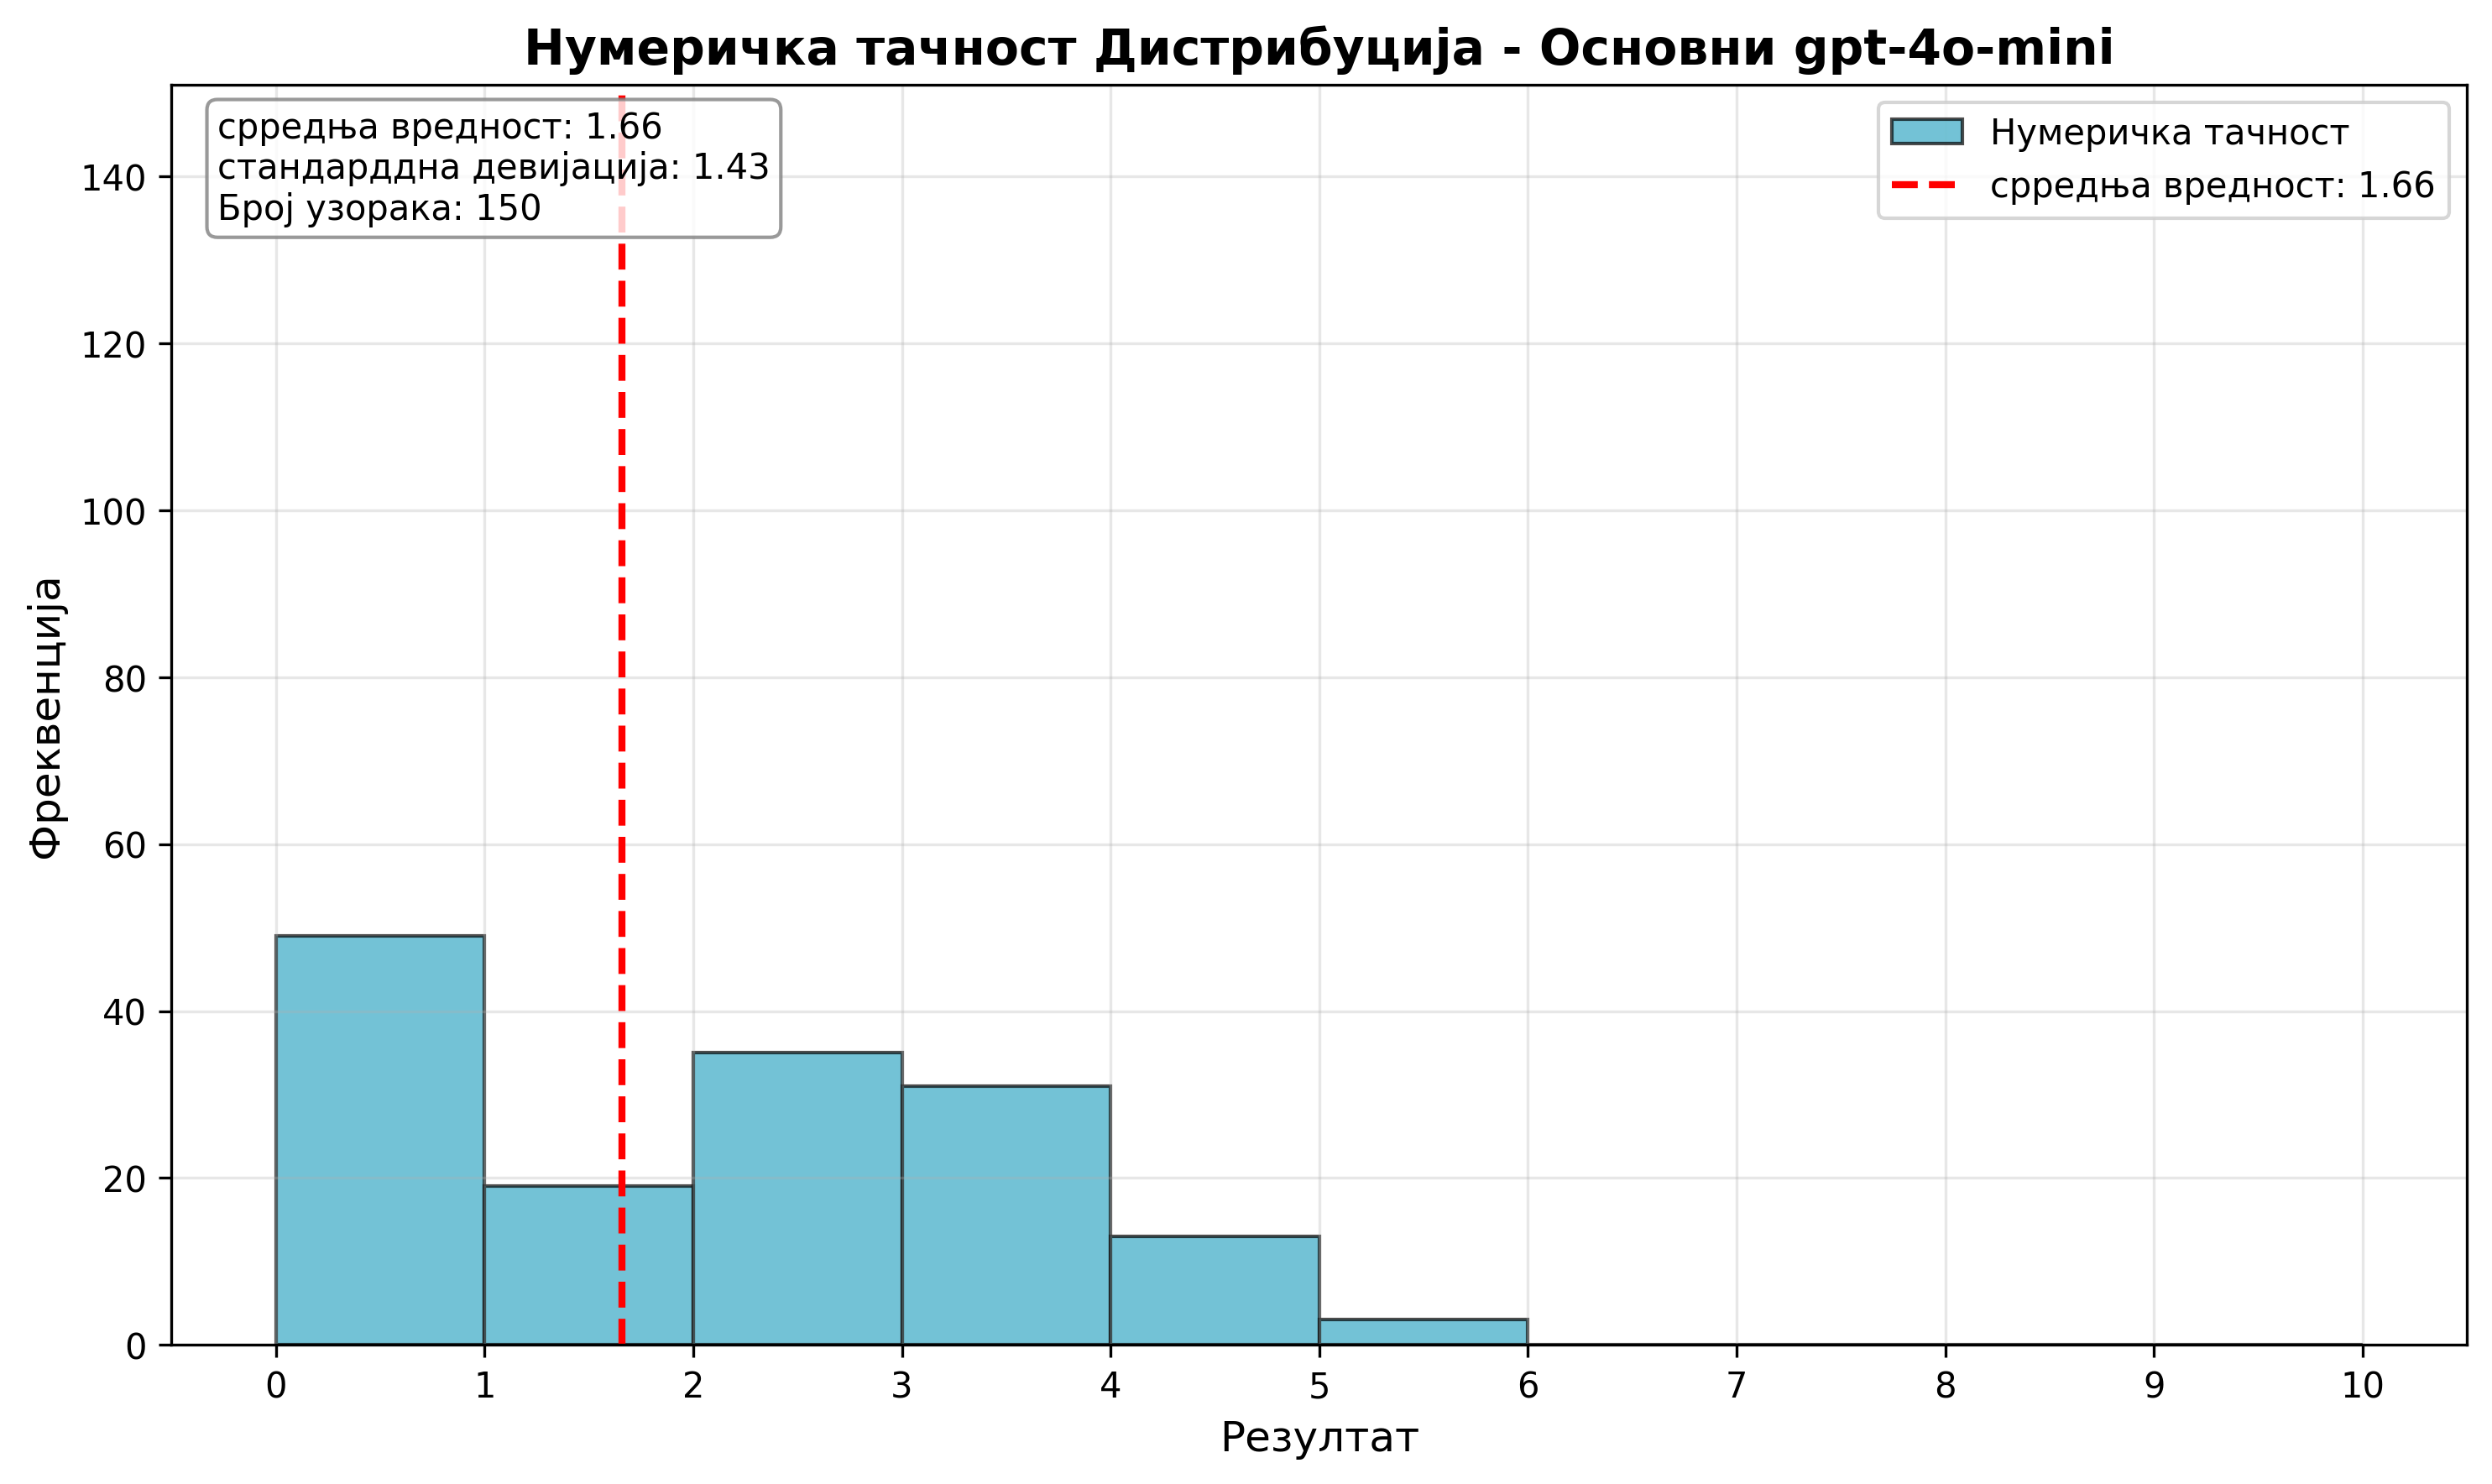
\includegraphics[width=0.8\textwidth]{images/osnovni/criteria_analysis_numerical_accuracy_histogram.png}
    
    \vspace{0.5cm}
    
    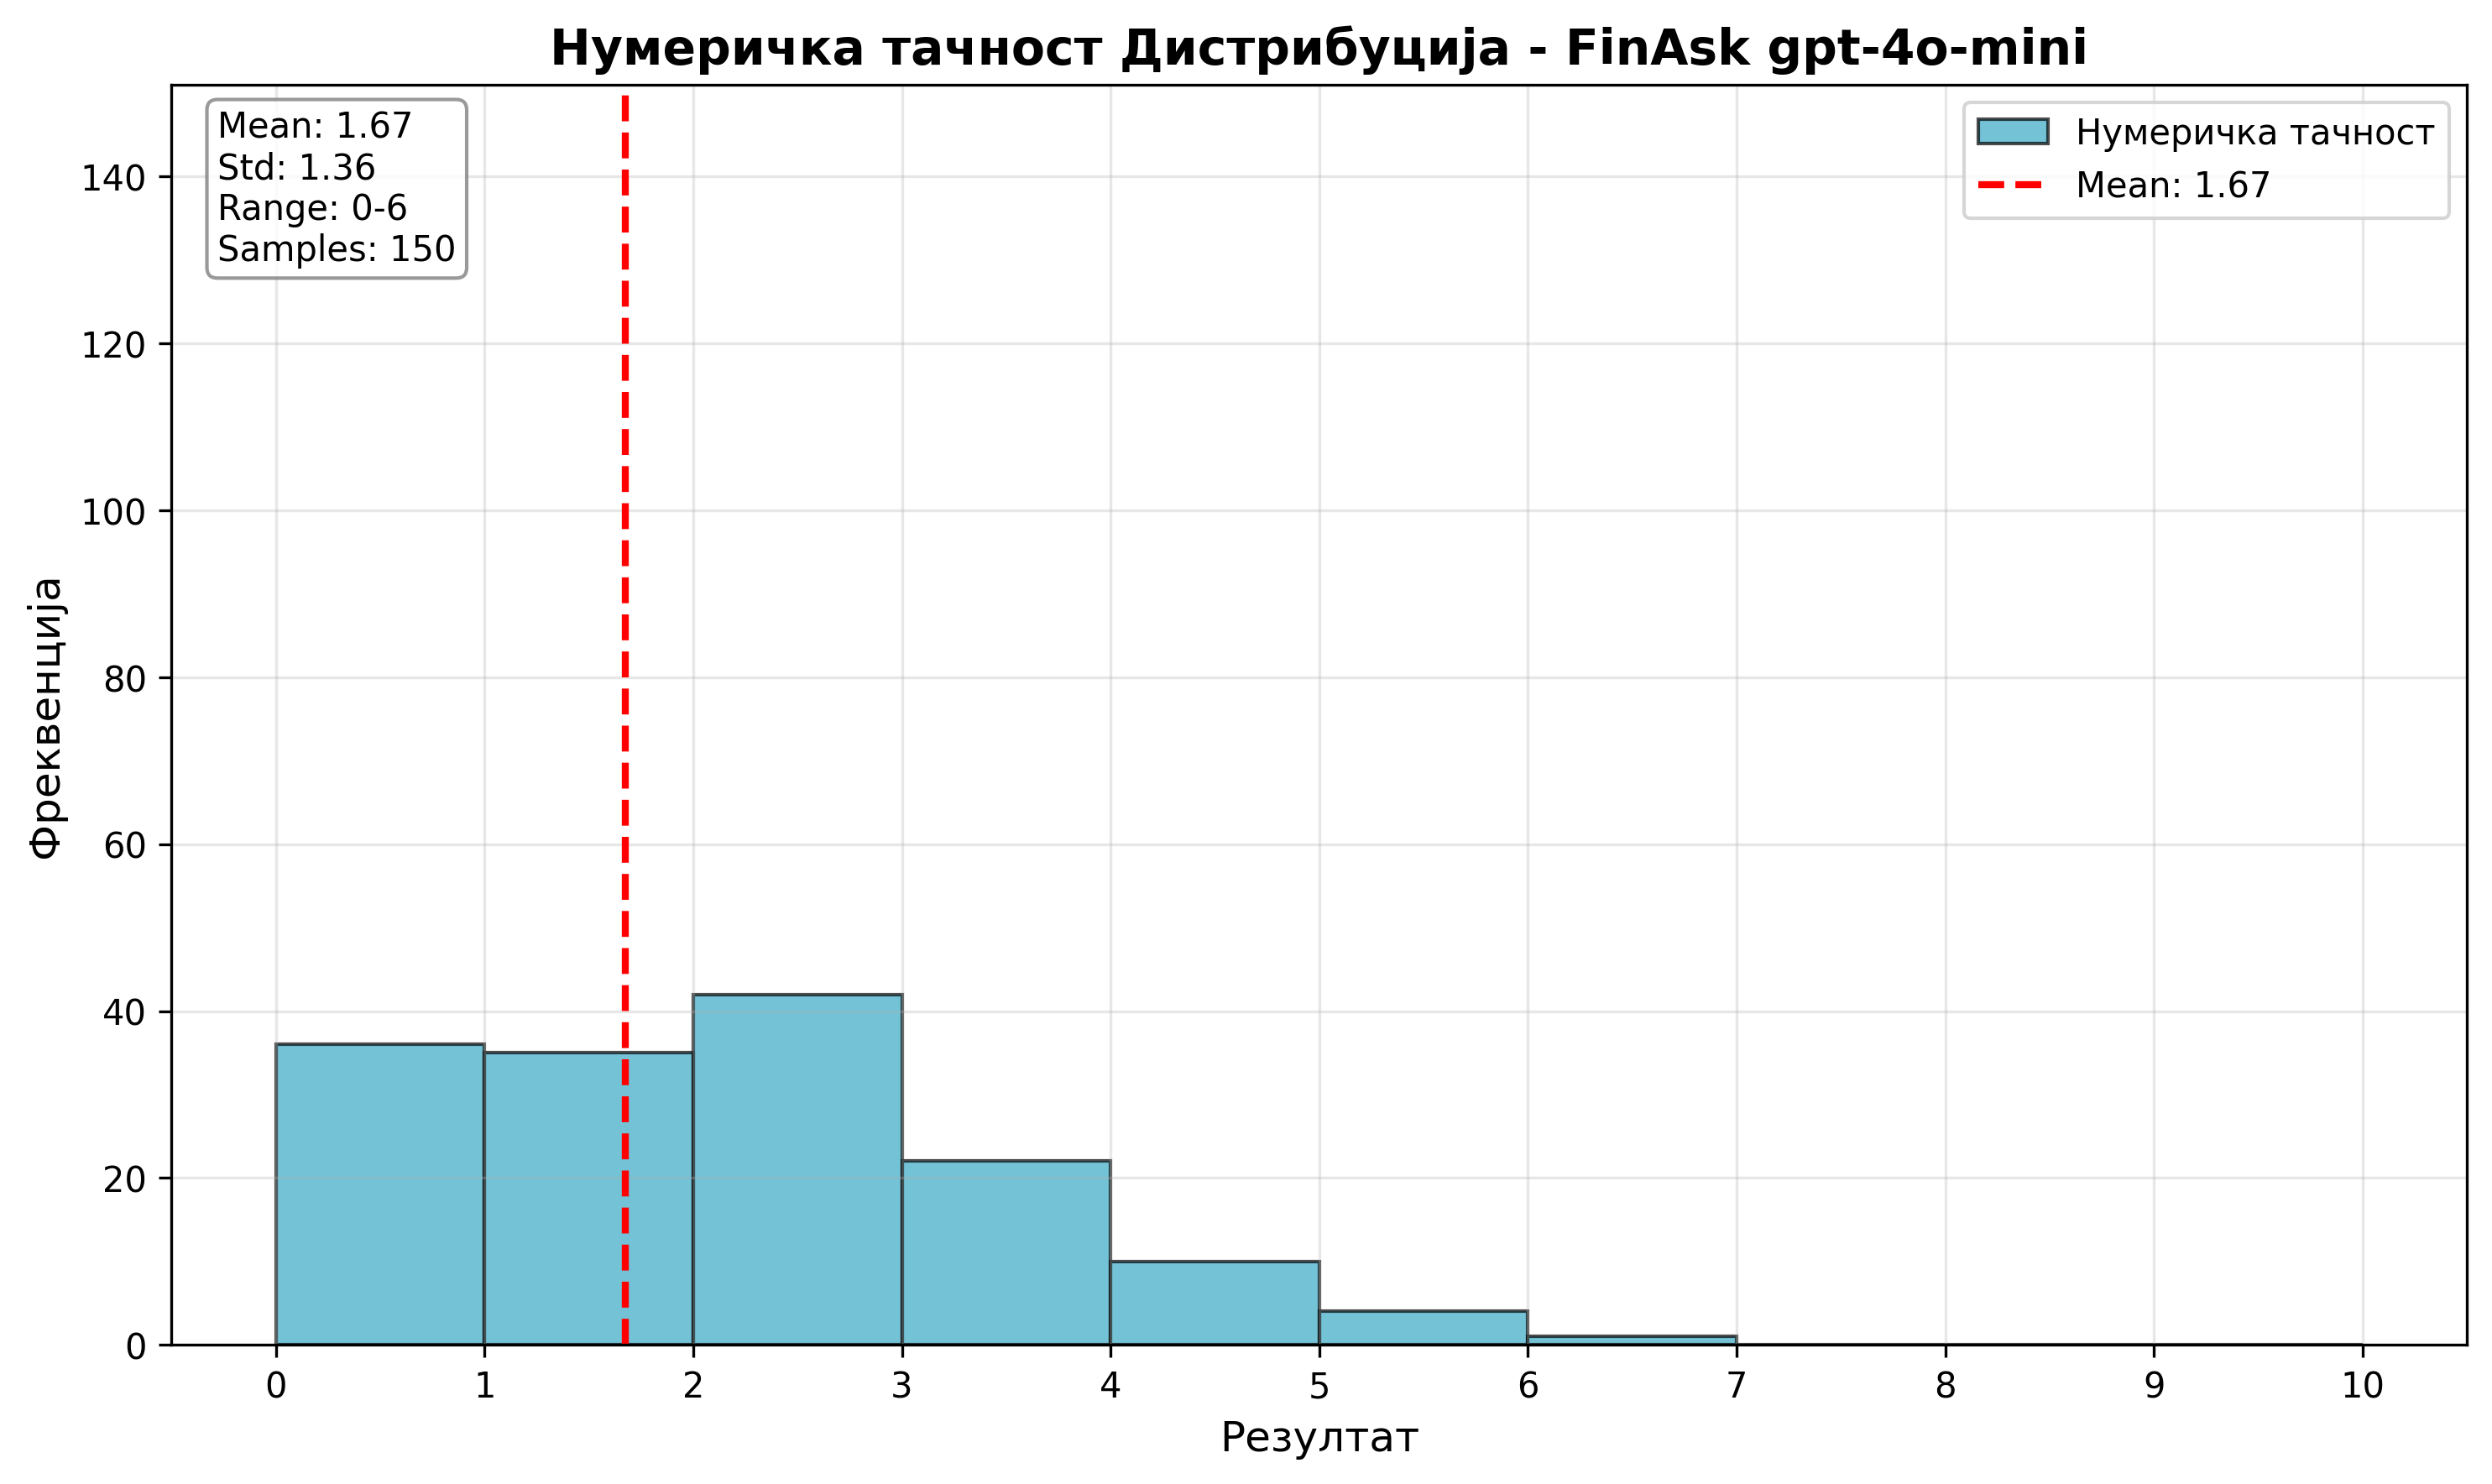
\includegraphics[width=0.8\textwidth]{images/FinAsk/criteria_analysis_numerical_accuracy_histogram.png}
    \caption{Хистограм анализе критеријума нумеричке тачности - горе: основни модел, доле: FinAsk модел}
    \label{fig:comparison_numerical}
\end{figure}
\chapter{Закључак}

У овом раду представљен је систем финансијског агента који користи велики језички модел (LLM) као судију за евалуацију својих одговора на финансијска питања. Главни циљ рада био је да се испита ефикасност овог приступа у побољшању квалитета одговора кроз прилагођавање промпта и ефикасност коришћења LLM-а као судије.
\newline

Резултати су показали значајно побољшање у тачности одговора када је коришћен прилагођени промпт у поређењу са основним моделом. Међутим није јасно да ли је агент показао могућност резоновања или је само боље проналазио информације у контексту. Поготово ако узмемо у обзир друге метрике где није било значајне разлике. Потребно је урадити дубљу анализу како би се утврдило да ли је побољшање последица бољег резоновања или само боље претраге информација. У будућности је потребно осмислити методологију која би подигла ниво тачности на виши ниво. Такође је потребна анализа колико су изабрани алати учинковити и да ли би избор других алата могао донети боље резултате.
\newline

Што се тиче коришћења LLM-а као судије, резултати основног модела су конзистентни са тачношћу  у истраживању које је урађено на оргиналном FinanceBench скупу података \cite{yang_evaluating_2025}, што указује на потенцијал овог приступа. За остале критеријуме је тешко одредити ефикасност овог приступа јер метрике могу бити субјективне. Потребно је урадити додатни преглед како би се боље разумело колико је LLM као судија поуздан у процени квалитета одговора. Генерално, упитно је колико се судија ослања на референтни одговор, а колико на своје знање и да ли је референтни одговор једини прави начин да се одговори на дато питање.
\newline




\cleardoublepage
\chapter*{Списак скраћеница}
\addcontentsline{toc}{chapter}{Списак скраћеница}

% Листа скраћеница по алфабетском реду
\begin{itemize}
    \item \textbf{API} -- Интерфејс за програмирање апликација (енг. \textit{Application Programming Interface})
    \item \textbf{ВЈМ} -- Велики језички модели (енг. \textit{Large Language Models - LLM})
    \item \textbf{BPE} -- Кодирање парова бајтова (енг. \textit{Byte Pair Encoding})
    \item \textbf{EDGAR} -- Програм електронског прикупљања, анализе и повлачења (енг. \textit{Electronic Data Gathering, Analysis, and Retrieval})
    \item \textbf{EPS} -- Зарада по акцији (енг. \textit{Earnings Per Share})
    \item \textbf{GPT} -- Генеративни претренирани трансформер (енг. \textit{Generative Pre-trained Transformer})
    \item \textbf{JSON} -- JavaScript објект нотација (енг. \textit{JavaScript Object Notation})
    \item \textbf{KPI} -- Кључни показатељи перформанси (енг. \textit{Key Performance Indicators})
    \item \textbf{LangChain} -- Отворени оквир за оркестрацију LLM апликација
    \item \textbf{LLM} -- Велики језички модели (енг. \textit{Large Language Models})
    \item \textbf{MSA} -- Вишеглави механизам пажње (енг. \textit{Multi-head Self-Attention})
    \item \textbf{NLP} -- Обрада природног језика (енг. \textit{Natural Language Processing})
    \item \textbf{PE} -- Позиционо кодирање (енг. \textit{Positional Encoding})
    \item \textbf{ППНМ} -- Потпуно повезане неуронске мреже (енг. \textit{Fully Connected Neural Networks})
    \item \textbf{Python} -- Програмски језик високог нивоа
    \item \textbf{RAG} -- Генерисање проширено преузимањем (енг. \textit{Retrieval-Augmented Generation})
    \item \textbf{ReAct} -- Резоновање и делање (енг. \textit{Reasoning and Acting})
    \item \textbf{ROA} -- Повраћај на активу (енг. \textit{Return on Assets})
    \item \textbf{ROE} -- Повраћај на капитал (енг. \textit{Return on Equity})
    \item \textbf{SDK} -- Комплет за развој софтвера (енг. \textit{Software Development Kit})
    \item \textbf{SEC} -- Комисија за хартије од вредности САД (енг. \textit{Securities and Exchange Commission})
    \item \textbf{10-K} -- Годишњи извештај америчких јавних компанија (енг. \textit{Form 10-K})
    \item \textbf{10-Q} -- Квартални извештај америчких јавних компанија (енг. \textit{Form 10-Q})
\end{itemize}

\cleardoublepage
\phantomsection
\addcontentsline{toc}{chapter}{Списак табела}
\listoftables

\cleardoublepage
\phantomsection
\addcontentsline{toc}{chapter}{Списак слика}
\listoffigures


\chapter{Додатак}
\label{appendix:llm_judge_prompt}

\begin{center}
    \begin{listing}[!ht]
    \footnotesize
    \begin{verbatim}

You are an expert financial analyst and judge evaluating answers to financial questions based 
on company 10-K filings.

QUESTION:
{question}

CANDIDATE ANSWER (to evaluate):
{candidate_answer}

REFERENCE ANSWER (expert baseline):
{reference_answer}

{context_info}

EVALUATION CRITERIA:
1. **Factual Correctness (0-10)**: Are all financial facts, numbers, and claims accurate?
   - Compare specific figures, percentages, and metrics
   - Verify calculations and data points
   - Check for consistency with reference answer

2. **Completeness (0-10)**: Does the answer address all aspects of the question?
   - Consider all parts of the original question
   - Evaluate depth and breadth of coverage
   - Compare against reference answer scope

3. **Financial Reasoning (0-10)**: Is the reasoning process sound and financially literate?
   - Assess analytical approach and methodology
   - Evaluate logical flow and financial principles
   - Consider appropriateness of conclusions

4. **Numerical Accuracy (0-10)**: Are calculations and financial figures correct?
   - Verify mathematical computations
   - Check ratios, percentages, and metrics
   - Assess precision and units

5. **Clarity (0-10)**: Is the answer clear, well-structured, and easy to understand?
   - Evaluate communication effectiveness
   - Assess structure and organization
   - Consider professional presentation

    \end{verbatim}
    \end{listing}
    \end{center}


   \begin{center}
    \begin{listing}[!ht]
    \footnotesize
    \begin{verbatim}

EVALUATION GUIDELINES:
- Use the reference answer as the gold standard for comparison
- Consider the expert correctness and completeness rationale provided
- Be aware of the original methodology and system prompt used
- Focus on substance over style but maintain professional standards
- Allow for reasonable differences in expression while maintaining accuracy
- Provide specific, actionable feedback with examples

Provide your evaluation as a JSON object with the following structure:
{{
  "factual_correctness": {{
    "score": <0-10>,
    "explanation": "<detailed explanation with specific examples>"
  }},
  "completeness": {{
    "score": <0-10>,
    "explanation": "<detailed explanation comparing coverage>"
  }},
  "financial_reasoning": {{
    "score": <0-10>,
    "explanation": "<assessment of analytical approach>"
  }},
  "numerical_accuracy": {{
    "score": <0-10>,
    "explanation": "<verification of calculations and figures>"
  }},
  "clarity": {{
    "score": <0-10>,
    "explanation": "<assessment of communication effectiveness>"
  }},
  "overall_score": <0-10>,
  "overall_explanation": "<comprehensive assessment highlighting key strengths and weaknesses>",
  "confidence": <0-1>,
  "key_differences": ["<list of key differences from reference>"]
}}

Be thorough, fair, and provide actionable feedback.
    \end{verbatim}
    \caption{Шаблон за рад агента судије}\label{lst:judge_template}
    \end{listing}
    \end{center}

\bibliographystyle{ieeetr}
\bibliography{master_rad}
%\addcontentsline{toc}{chapter}{Литература}

% Alternativni način
%\begin{thebibliography}{10}
%\bibitem{Shalev-Shwartz:2014:UML:2621980}
%S. Shalev-Shwartz, S. Ben-David, \emph{Understanding MachineLearning}, Cambridge, 2016
%\end{thebibliography}

\end{document}